\documentclass[twoside]{book}

% Packages required by doxygen
\usepackage{calc}
\usepackage{doxygen}
\usepackage{graphicx}
\usepackage[utf8]{inputenc}
\usepackage{makeidx}
\usepackage{multicol}
\usepackage{multirow}
\usepackage{textcomp}
\usepackage[table]{xcolor}

% Font selection
\usepackage[T1]{fontenc}
\usepackage{mathptmx}
\usepackage[scaled=.90]{helvet}
\usepackage{courier}
\usepackage{amssymb}
\usepackage{sectsty}
\renewcommand{\familydefault}{\sfdefault}
\allsectionsfont{%
  \fontseries{bc}\selectfont%
  \color{darkgray}%
}
\renewcommand{\DoxyLabelFont}{%
  \fontseries{bc}\selectfont%
  \color{darkgray}%
}

% Page & text layout
\usepackage{geometry}
\geometry{%
  a4paper,%
  top=2.5cm,%
  bottom=2.5cm,%
  left=2.5cm,%
  right=2.5cm%
}
\tolerance=750
\hfuzz=15pt
\hbadness=750
\setlength{\emergencystretch}{15pt}
\setlength{\parindent}{0cm}
\setlength{\parskip}{0.2cm}
\makeatletter
\renewcommand{\paragraph}{%
  \@startsection{paragraph}{4}{0ex}{-1.0ex}{1.0ex}{%
    \normalfont\normalsize\bfseries\SS@parafont%
  }%
}
\renewcommand{\subparagraph}{%
  \@startsection{subparagraph}{5}{0ex}{-1.0ex}{1.0ex}{%
    \normalfont\normalsize\bfseries\SS@subparafont%
  }%
}
\makeatother

% Headers & footers
\usepackage{fancyhdr}
\pagestyle{fancyplain}
\fancyhead[LE]{\fancyplain{}{\bfseries\thepage}}
\fancyhead[CE]{\fancyplain{}{}}
\fancyhead[RE]{\fancyplain{}{\bfseries\leftmark}}
\fancyhead[LO]{\fancyplain{}{\bfseries\rightmark}}
\fancyhead[CO]{\fancyplain{}{}}
\fancyhead[RO]{\fancyplain{}{\bfseries\thepage}}
\fancyfoot[LE]{\fancyplain{}{}}
\fancyfoot[CE]{\fancyplain{}{}}
\fancyfoot[RE]{\fancyplain{}{\bfseries\scriptsize Generated on Wed May 4 2016 21\-:08\-:09 for My Project by Doxygen }}
\fancyfoot[LO]{\fancyplain{}{\bfseries\scriptsize Generated on Wed May 4 2016 21\-:08\-:09 for My Project by Doxygen }}
\fancyfoot[CO]{\fancyplain{}{}}
\fancyfoot[RO]{\fancyplain{}{}}
\renewcommand{\footrulewidth}{0.4pt}
\renewcommand{\chaptermark}[1]{%
  \markboth{#1}{}%
}
\renewcommand{\sectionmark}[1]{%
  \markright{\thesection\ #1}%
}

% Indices & bibliography
\usepackage{natbib}
\usepackage[titles]{tocloft}
\setcounter{tocdepth}{3}
\setcounter{secnumdepth}{5}
\makeindex

% Hyperlinks (required, but should be loaded last)
\usepackage{ifpdf}
\ifpdf
  \usepackage[pdftex,pagebackref=true]{hyperref}
\else
  \usepackage[ps2pdf,pagebackref=true]{hyperref}
\fi
\hypersetup{%
  colorlinks=true,%
  linkcolor=blue,%
  citecolor=blue,%
  unicode%
}

% Custom commands
\newcommand{\clearemptydoublepage}{%
  \newpage{\pagestyle{empty}\cleardoublepage}%
}


%===== C O N T E N T S =====

\begin{document}

% Titlepage & ToC
\hypersetup{pageanchor=false}
\pagenumbering{roman}
\begin{titlepage}
\vspace*{7cm}
\begin{center}%
{\Large My Project }\\
\vspace*{1cm}
{\large Generated by Doxygen 1.8.6}\\
\vspace*{0.5cm}
{\small Wed May 4 2016 21:08:09}\\
\end{center}
\end{titlepage}
\clearemptydoublepage
\tableofcontents
\clearemptydoublepage
\pagenumbering{arabic}
\hypersetup{pageanchor=true}

%--- Begin generated contents ---
\chapter{Hierarchical Index}
\section{Class Hierarchy}
This inheritance list is sorted roughly, but not completely, alphabetically\-:\begin{DoxyCompactList}
\item \contentsline{section}{Base\-Gfx\-App}{\pageref{classBaseGfxApp}}{}
\begin{DoxyCompactList}
\item \contentsline{section}{Flash\-Photo\-App}{\pageref{classFlashPhotoApp}}{}
\item \contentsline{section}{M\-I\-A\-App}{\pageref{classMIAApp}}{}
\end{DoxyCompactList}
\item \contentsline{section}{Color\-Data}{\pageref{classColorData}}{}
\item \contentsline{section}{Draw\-Tool}{\pageref{classDrawTool}}{}
\begin{DoxyCompactList}
\item \contentsline{section}{Blur}{\pageref{classBlur}}{}
\item \contentsline{section}{Calligraphy\-Pen}{\pageref{classCalligraphyPen}}{}
\item \contentsline{section}{Crayon}{\pageref{classCrayon}}{}
\item \contentsline{section}{Eraser}{\pageref{classEraser}}{}
\item \contentsline{section}{Fill\-Tool}{\pageref{classFillTool}}{}
\item \contentsline{section}{Highlighter}{\pageref{classHighlighter}}{}
\item \contentsline{section}{Pen}{\pageref{classPen}}{}
\item \contentsline{section}{Spray\-Can}{\pageref{classSprayCan}}{}
\item \contentsline{section}{Stamp}{\pageref{classStamp}}{}
\item \contentsline{section}{Water\-Color}{\pageref{classWaterColor}}{}
\end{DoxyCompactList}
\item \contentsline{section}{Filter}{\pageref{classFilter}}{}
\begin{DoxyCompactList}
\item \contentsline{section}{F\-Blur}{\pageref{classFBlur}}{}
\begin{DoxyCompactList}
\item \contentsline{section}{F\-Edge\-Detection}{\pageref{classFEdgeDetection}}{}
\item \contentsline{section}{F\-Motion\-Blur}{\pageref{classFMotionBlur}}{}
\item \contentsline{section}{F\-Sharpen}{\pageref{classFSharpen}}{}
\end{DoxyCompactList}
\item \contentsline{section}{F\-Channel}{\pageref{classFChannel}}{}
\item \contentsline{section}{F\-Quantize}{\pageref{classFQuantize}}{}
\item \contentsline{section}{F\-Saturation}{\pageref{classFSaturation}}{}
\item \contentsline{section}{F\-Special}{\pageref{classFSpecial}}{}
\item \contentsline{section}{F\-Threshold}{\pageref{classFThreshold}}{}
\end{DoxyCompactList}
\item \contentsline{section}{Filter\-Factory}{\pageref{classFilterFactory}}{}
\item \contentsline{section}{Image\-Handler}{\pageref{classImageHandler}}{}
\item \contentsline{section}{Mask}{\pageref{classMask}}{}
\item \contentsline{section}{M\-I\-A\-Command\-Line\-App}{\pageref{classMIACommandLineApp}}{}
\item \contentsline{section}{Pixel\-Buffer}{\pageref{classPixelBuffer}}{}
\end{DoxyCompactList}

\chapter{Class Index}
\section{Class List}
Here are the classes, structs, unions and interfaces with brief descriptions\-:\begin{DoxyCompactList}
\item\contentsline{section}{\hyperlink{struct__mainprog__info}{\-\_\-mainprog\-\_\-info} }{\pageref{struct__mainprog__info}}{}
\item\contentsline{section}{\hyperlink{classArcball}{Arcball} }{\pageref{classArcball}}{}
\item\contentsline{section}{\hyperlink{structbacking__store__struct}{backing\-\_\-store\-\_\-struct} }{\pageref{structbacking__store__struct}}{}
\item\contentsline{section}{\hyperlink{classBaseGfxApp}{Base\-Gfx\-App} }{\pageref{classBaseGfxApp}}{}
\item\contentsline{section}{\hyperlink{classBlur}{Blur} }{\pageref{classBlur}}{}
\item\contentsline{section}{\hyperlink{classCalligraphyPen}{Calligraphy\-Pen} }{\pageref{classCalligraphyPen}}{}
\item\contentsline{section}{\hyperlink{structcdjpeg__progress__mgr}{cdjpeg\-\_\-progress\-\_\-mgr} }{\pageref{structcdjpeg__progress__mgr}}{}
\item\contentsline{section}{\hyperlink{structcjpeg__source__struct}{cjpeg\-\_\-source\-\_\-struct} }{\pageref{structcjpeg__source__struct}}{}
\item\contentsline{section}{\hyperlink{classColorData}{Color\-Data} }{\pageref{classColorData}}{}
\item\contentsline{section}{\hyperlink{classCrayon}{Crayon} }{\pageref{classCrayon}}{}
\item\contentsline{section}{\hyperlink{structdjpeg__dest__struct}{djpeg\-\_\-dest\-\_\-struct} }{\pageref{structdjpeg__dest__struct}}{}
\item\contentsline{section}{\hyperlink{classDrawTool}{Draw\-Tool} }{\pageref{classDrawTool}}{}
\item\contentsline{section}{\hyperlink{classEraser}{Eraser} }{\pageref{classEraser}}{}
\item\contentsline{section}{\hyperlink{classFBlur}{F\-Blur} }{\pageref{classFBlur}}{}
\item\contentsline{section}{\hyperlink{classFChannel}{F\-Channel} }{\pageref{classFChannel}}{}
\item\contentsline{section}{\hyperlink{classFEdgeDetection}{F\-Edge\-Detection} }{\pageref{classFEdgeDetection}}{}
\item\contentsline{section}{\hyperlink{classFillTool}{Fill\-Tool} }{\pageref{classFillTool}}{}
\item\contentsline{section}{\hyperlink{classFilter}{Filter} }{\pageref{classFilter}}{}
\item\contentsline{section}{\hyperlink{classFilterFactory}{Filter\-Factory} }{\pageref{classFilterFactory}}{}
\item\contentsline{section}{\hyperlink{classFlashPhotoApp}{Flash\-Photo\-App} }{\pageref{classFlashPhotoApp}}{}
\item\contentsline{section}{\hyperlink{classFMotionBlur}{F\-Motion\-Blur} }{\pageref{classFMotionBlur}}{}
\item\contentsline{section}{\hyperlink{classFQuantize}{F\-Quantize} }{\pageref{classFQuantize}}{}
\item\contentsline{section}{\hyperlink{classFSaturation}{F\-Saturation} }{\pageref{classFSaturation}}{}
\item\contentsline{section}{\hyperlink{classFSharpen}{F\-Sharpen} }{\pageref{classFSharpen}}{}
\item\contentsline{section}{\hyperlink{classFSpecial}{F\-Special} }{\pageref{classFSpecial}}{}
\item\contentsline{section}{\hyperlink{classFThreshold}{F\-Threshold} }{\pageref{classFThreshold}}{}
\item\contentsline{section}{\hyperlink{classGLUI}{G\-L\-U\-I} }{\pageref{classGLUI}}{}
\item\contentsline{section}{\hyperlink{classGLUI__Bitmap}{G\-L\-U\-I\-\_\-\-Bitmap} }{\pageref{classGLUI__Bitmap}}{}
\item\contentsline{section}{\hyperlink{classGLUI__Button}{G\-L\-U\-I\-\_\-\-Button} }{\pageref{classGLUI__Button}}{}
\item\contentsline{section}{\hyperlink{classGLUI__CB}{G\-L\-U\-I\-\_\-\-C\-B} }{\pageref{classGLUI__CB}}{}
\item\contentsline{section}{\hyperlink{classGLUI__Checkbox}{G\-L\-U\-I\-\_\-\-Checkbox} }{\pageref{classGLUI__Checkbox}}{}
\item\contentsline{section}{\hyperlink{classGLUI__Column}{G\-L\-U\-I\-\_\-\-Column} }{\pageref{classGLUI__Column}}{}
\item\contentsline{section}{\hyperlink{classGLUI__CommandLine}{G\-L\-U\-I\-\_\-\-Command\-Line} }{\pageref{classGLUI__CommandLine}}{}
\item\contentsline{section}{\hyperlink{classGLUI__Control}{G\-L\-U\-I\-\_\-\-Control} }{\pageref{classGLUI__Control}}{}
\item\contentsline{section}{\hyperlink{classGLUI__DrawingSentinal}{G\-L\-U\-I\-\_\-\-Drawing\-Sentinal} }{\pageref{classGLUI__DrawingSentinal}}{}
\item\contentsline{section}{\hyperlink{classGLUI__EditText}{G\-L\-U\-I\-\_\-\-Edit\-Text} }{\pageref{classGLUI__EditText}}{}
\item\contentsline{section}{\hyperlink{classGLUI__FileBrowser}{G\-L\-U\-I\-\_\-\-File\-Browser} }{\pageref{classGLUI__FileBrowser}}{}
\item\contentsline{section}{\hyperlink{classGLUI__Glut__Window}{G\-L\-U\-I\-\_\-\-Glut\-\_\-\-Window} }{\pageref{classGLUI__Glut__Window}}{}
\item\contentsline{section}{\hyperlink{classGLUI__List}{G\-L\-U\-I\-\_\-\-List} }{\pageref{classGLUI__List}}{}
\item\contentsline{section}{\hyperlink{classGLUI__List__Item}{G\-L\-U\-I\-\_\-\-List\-\_\-\-Item} }{\pageref{classGLUI__List__Item}}{}
\item\contentsline{section}{\hyperlink{classGLUI__Listbox}{G\-L\-U\-I\-\_\-\-Listbox} }{\pageref{classGLUI__Listbox}}{}
\item\contentsline{section}{\hyperlink{classGLUI__Listbox__Item}{G\-L\-U\-I\-\_\-\-Listbox\-\_\-\-Item} }{\pageref{classGLUI__Listbox__Item}}{}
\item\contentsline{section}{\hyperlink{classGLUI__Main}{G\-L\-U\-I\-\_\-\-Main} }{\pageref{classGLUI__Main}}{}
\item\contentsline{section}{\hyperlink{classGLUI__Master__Object}{G\-L\-U\-I\-\_\-\-Master\-\_\-\-Object} }{\pageref{classGLUI__Master__Object}}{}
\item\contentsline{section}{\hyperlink{classGLUI__Mouse__Interaction}{G\-L\-U\-I\-\_\-\-Mouse\-\_\-\-Interaction} }{\pageref{classGLUI__Mouse__Interaction}}{}
\item\contentsline{section}{\hyperlink{classGLUI__Node}{G\-L\-U\-I\-\_\-\-Node} }{\pageref{classGLUI__Node}}{}
\item\contentsline{section}{\hyperlink{classGLUI__Panel}{G\-L\-U\-I\-\_\-\-Panel} }{\pageref{classGLUI__Panel}}{}
\item\contentsline{section}{\hyperlink{classGLUI__RadioButton}{G\-L\-U\-I\-\_\-\-Radio\-Button} }{\pageref{classGLUI__RadioButton}}{}
\item\contentsline{section}{\hyperlink{classGLUI__RadioGroup}{G\-L\-U\-I\-\_\-\-Radio\-Group} }{\pageref{classGLUI__RadioGroup}}{}
\item\contentsline{section}{\hyperlink{classGLUI__Rollout}{G\-L\-U\-I\-\_\-\-Rollout} }{\pageref{classGLUI__Rollout}}{}
\item\contentsline{section}{\hyperlink{classGLUI__Rotation}{G\-L\-U\-I\-\_\-\-Rotation} }{\pageref{classGLUI__Rotation}}{}
\item\contentsline{section}{\hyperlink{classGLUI__Scrollbar}{G\-L\-U\-I\-\_\-\-Scrollbar} }{\pageref{classGLUI__Scrollbar}}{}
\item\contentsline{section}{\hyperlink{classGLUI__Separator}{G\-L\-U\-I\-\_\-\-Separator} }{\pageref{classGLUI__Separator}}{}
\item\contentsline{section}{\hyperlink{classGLUI__Spinner}{G\-L\-U\-I\-\_\-\-Spinner} }{\pageref{classGLUI__Spinner}}{}
\item\contentsline{section}{\hyperlink{classGLUI__StaticText}{G\-L\-U\-I\-\_\-\-Static\-Text} }{\pageref{classGLUI__StaticText}}{}
\item\contentsline{section}{\hyperlink{classGLUI__StdBitmaps}{G\-L\-U\-I\-\_\-\-Std\-Bitmaps} }{\pageref{classGLUI__StdBitmaps}}{}
\item\contentsline{section}{\hyperlink{classGLUI__TextBox}{G\-L\-U\-I\-\_\-\-Text\-Box} }{\pageref{classGLUI__TextBox}}{}
\item\contentsline{section}{\hyperlink{classGLUI__Translation}{G\-L\-U\-I\-\_\-\-Translation} }{\pageref{classGLUI__Translation}}{}
\item\contentsline{section}{\hyperlink{classGLUI__Tree}{G\-L\-U\-I\-\_\-\-Tree} }{\pageref{classGLUI__Tree}}{}
\item\contentsline{section}{\hyperlink{classGLUI__TreePanel}{G\-L\-U\-I\-\_\-\-Tree\-Panel} }{\pageref{classGLUI__TreePanel}}{}
\item\contentsline{section}{\hyperlink{classHighlighter}{Highlighter} }{\pageref{classHighlighter}}{}
\item\contentsline{section}{\hyperlink{classImageHandler}{Image\-Handler} }{\pageref{classImageHandler}}{}
\item\contentsline{section}{\hyperlink{structJHUFF__TBL}{J\-H\-U\-F\-F\-\_\-\-T\-B\-L} }{\pageref{structJHUFF__TBL}}{}
\item\contentsline{section}{\hyperlink{structjpeg__c__coef__controller}{jpeg\-\_\-c\-\_\-coef\-\_\-controller} }{\pageref{structjpeg__c__coef__controller}}{}
\item\contentsline{section}{\hyperlink{structjpeg__c__main__controller}{jpeg\-\_\-c\-\_\-main\-\_\-controller} }{\pageref{structjpeg__c__main__controller}}{}
\item\contentsline{section}{\hyperlink{structjpeg__c__prep__controller}{jpeg\-\_\-c\-\_\-prep\-\_\-controller} }{\pageref{structjpeg__c__prep__controller}}{}
\item\contentsline{section}{\hyperlink{structjpeg__color__converter}{jpeg\-\_\-color\-\_\-converter} }{\pageref{structjpeg__color__converter}}{}
\item\contentsline{section}{\hyperlink{structjpeg__color__deconverter}{jpeg\-\_\-color\-\_\-deconverter} }{\pageref{structjpeg__color__deconverter}}{}
\item\contentsline{section}{\hyperlink{structjpeg__color__quantizer}{jpeg\-\_\-color\-\_\-quantizer} }{\pageref{structjpeg__color__quantizer}}{}
\item\contentsline{section}{\hyperlink{structjpeg__common__struct}{jpeg\-\_\-common\-\_\-struct} }{\pageref{structjpeg__common__struct}}{}
\item\contentsline{section}{\hyperlink{structjpeg__comp__master}{jpeg\-\_\-comp\-\_\-master} }{\pageref{structjpeg__comp__master}}{}
\item\contentsline{section}{\hyperlink{structjpeg__component__info}{jpeg\-\_\-component\-\_\-info} }{\pageref{structjpeg__component__info}}{}
\item\contentsline{section}{\hyperlink{structjpeg__compress__struct}{jpeg\-\_\-compress\-\_\-struct} }{\pageref{structjpeg__compress__struct}}{}
\item\contentsline{section}{\hyperlink{structjpeg__d__coef__controller}{jpeg\-\_\-d\-\_\-coef\-\_\-controller} }{\pageref{structjpeg__d__coef__controller}}{}
\item\contentsline{section}{\hyperlink{structjpeg__d__main__controller}{jpeg\-\_\-d\-\_\-main\-\_\-controller} }{\pageref{structjpeg__d__main__controller}}{}
\item\contentsline{section}{\hyperlink{structjpeg__d__post__controller}{jpeg\-\_\-d\-\_\-post\-\_\-controller} }{\pageref{structjpeg__d__post__controller}}{}
\item\contentsline{section}{\hyperlink{structjpeg__decomp__master}{jpeg\-\_\-decomp\-\_\-master} }{\pageref{structjpeg__decomp__master}}{}
\item\contentsline{section}{\hyperlink{structjpeg__decompress__struct}{jpeg\-\_\-decompress\-\_\-struct} }{\pageref{structjpeg__decompress__struct}}{}
\item\contentsline{section}{\hyperlink{structjpeg__destination__mgr}{jpeg\-\_\-destination\-\_\-mgr} }{\pageref{structjpeg__destination__mgr}}{}
\item\contentsline{section}{\hyperlink{structjpeg__downsampler}{jpeg\-\_\-downsampler} }{\pageref{structjpeg__downsampler}}{}
\item\contentsline{section}{\hyperlink{structjpeg__entropy__decoder}{jpeg\-\_\-entropy\-\_\-decoder} }{\pageref{structjpeg__entropy__decoder}}{}
\item\contentsline{section}{\hyperlink{structjpeg__entropy__encoder}{jpeg\-\_\-entropy\-\_\-encoder} }{\pageref{structjpeg__entropy__encoder}}{}
\item\contentsline{section}{\hyperlink{structjpeg__error__mgr}{jpeg\-\_\-error\-\_\-mgr} }{\pageref{structjpeg__error__mgr}}{}
\item\contentsline{section}{\hyperlink{structjpeg__forward__dct}{jpeg\-\_\-forward\-\_\-dct} }{\pageref{structjpeg__forward__dct}}{}
\item\contentsline{section}{\hyperlink{structjpeg__input__controller}{jpeg\-\_\-input\-\_\-controller} }{\pageref{structjpeg__input__controller}}{}
\item\contentsline{section}{\hyperlink{structjpeg__inverse__dct}{jpeg\-\_\-inverse\-\_\-dct} }{\pageref{structjpeg__inverse__dct}}{}
\item\contentsline{section}{\hyperlink{structjpeg__marker__reader}{jpeg\-\_\-marker\-\_\-reader} }{\pageref{structjpeg__marker__reader}}{}
\item\contentsline{section}{\hyperlink{structjpeg__marker__struct}{jpeg\-\_\-marker\-\_\-struct} }{\pageref{structjpeg__marker__struct}}{}
\item\contentsline{section}{\hyperlink{structjpeg__marker__writer}{jpeg\-\_\-marker\-\_\-writer} }{\pageref{structjpeg__marker__writer}}{}
\item\contentsline{section}{\hyperlink{structjpeg__memory__mgr}{jpeg\-\_\-memory\-\_\-mgr} }{\pageref{structjpeg__memory__mgr}}{}
\item\contentsline{section}{\hyperlink{structjpeg__progress__mgr}{jpeg\-\_\-progress\-\_\-mgr} }{\pageref{structjpeg__progress__mgr}}{}
\item\contentsline{section}{\hyperlink{structjpeg__scan__info}{jpeg\-\_\-scan\-\_\-info} }{\pageref{structjpeg__scan__info}}{}
\item\contentsline{section}{\hyperlink{structjpeg__source__mgr}{jpeg\-\_\-source\-\_\-mgr} }{\pageref{structjpeg__source__mgr}}{}
\item\contentsline{section}{\hyperlink{structjpeg__transform__info}{jpeg\-\_\-transform\-\_\-info} }{\pageref{structjpeg__transform__info}}{}
\item\contentsline{section}{\hyperlink{structjpeg__upsampler}{jpeg\-\_\-upsampler} }{\pageref{structjpeg__upsampler}}{}
\item\contentsline{section}{\hyperlink{structJQUANT__TBL}{J\-Q\-U\-A\-N\-T\-\_\-\-T\-B\-L} }{\pageref{structJQUANT__TBL}}{}
\item\contentsline{section}{\hyperlink{classMask}{Mask} }{\pageref{classMask}}{}
\item\contentsline{section}{\hyperlink{classmat3}{mat3} }{\pageref{classmat3}}{}
\item\contentsline{section}{\hyperlink{classmat4}{mat4} }{\pageref{classmat4}}{}
\item\contentsline{section}{\hyperlink{classMIAApp}{M\-I\-A\-App} }{\pageref{classMIAApp}}{}
\item\contentsline{section}{\hyperlink{classPen}{Pen} }{\pageref{classPen}}{}
\item\contentsline{section}{\hyperlink{classPixelBuffer}{Pixel\-Buffer} }{\pageref{classPixelBuffer}}{}
\item\contentsline{section}{\hyperlink{structpng__color__16__struct}{png\-\_\-color\-\_\-16\-\_\-struct} }{\pageref{structpng__color__16__struct}}{}
\item\contentsline{section}{\hyperlink{structpng__color__8__struct}{png\-\_\-color\-\_\-8\-\_\-struct} }{\pageref{structpng__color__8__struct}}{}
\item\contentsline{section}{\hyperlink{structpng__color__struct}{png\-\_\-color\-\_\-struct} }{\pageref{structpng__color__struct}}{}
\item\contentsline{section}{\hyperlink{structpng__control}{png\-\_\-control} }{\pageref{structpng__control}}{}
\item\contentsline{section}{\hyperlink{structpng__image}{png\-\_\-image} }{\pageref{structpng__image}}{}
\item\contentsline{section}{\hyperlink{structpng__info__def}{png\-\_\-info\-\_\-def} }{\pageref{structpng__info__def}}{}
\item\contentsline{section}{\hyperlink{structpng__row__info__struct}{png\-\_\-row\-\_\-info\-\_\-struct} }{\pageref{structpng__row__info__struct}}{}
\item\contentsline{section}{\hyperlink{structpng__sPLT__entry__struct}{png\-\_\-s\-P\-L\-T\-\_\-entry\-\_\-struct} }{\pageref{structpng__sPLT__entry__struct}}{}
\item\contentsline{section}{\hyperlink{structpng__sPLT__struct}{png\-\_\-s\-P\-L\-T\-\_\-struct} }{\pageref{structpng__sPLT__struct}}{}
\item\contentsline{section}{\hyperlink{structpng__struct__def}{png\-\_\-struct\-\_\-def} }{\pageref{structpng__struct__def}}{}
\item\contentsline{section}{\hyperlink{structpng__text__struct}{png\-\_\-text\-\_\-struct} }{\pageref{structpng__text__struct}}{}
\item\contentsline{section}{\hyperlink{structpng__time__struct}{png\-\_\-time\-\_\-struct} }{\pageref{structpng__time__struct}}{}
\item\contentsline{section}{\hyperlink{structpng__unknown__chunk__t}{png\-\_\-unknown\-\_\-chunk\-\_\-t} }{\pageref{structpng__unknown__chunk__t}}{}
\item\contentsline{section}{\hyperlink{classquat}{quat} }{\pageref{classquat}}{}
\item\contentsline{section}{\hyperlink{classRGBc}{R\-G\-Bc} }{\pageref{classRGBc}}{}
\item\contentsline{section}{\hyperlink{classSprayCan}{Spray\-Can} }{\pageref{classSprayCan}}{}
\item\contentsline{section}{\hyperlink{classStamp}{Stamp} }{\pageref{classStamp}}{}
\item\contentsline{section}{\hyperlink{classvec2}{vec2} }{\pageref{classvec2}}{}
\item\contentsline{section}{\hyperlink{classvec3}{vec3} }{\pageref{classvec3}}{}
\item\contentsline{section}{\hyperlink{classvec4}{vec4} }{\pageref{classvec4}}{}
\item\contentsline{section}{\hyperlink{classViewModel}{View\-Model} }{\pageref{classViewModel}}{}
\item\contentsline{section}{\hyperlink{classWaterColor}{Water\-Color} }{\pageref{classWaterColor}}{}
\end{DoxyCompactList}

\chapter{Class Documentation}
\hypertarget{classBaseGfxApp}{\section{Base\-Gfx\-App Class Reference}
\label{classBaseGfxApp}\index{Base\-Gfx\-App@{Base\-Gfx\-App}}
}


{\ttfamily \#include $<$Base\-Gfx\-App.\-h$>$}

Inheritance diagram for Base\-Gfx\-App\-:\begin{figure}[H]
\begin{center}
\leavevmode
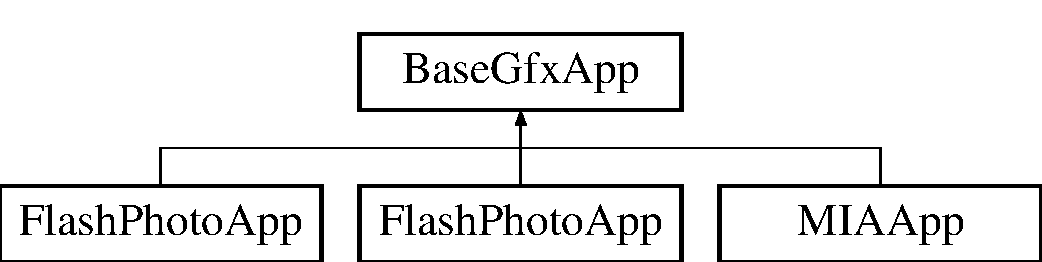
\includegraphics[height=2.000000cm]{classBaseGfxApp}
\end{center}
\end{figure}
\subsection*{Public Member Functions}
\begin{DoxyCompactItemize}
\item 
\hypertarget{classBaseGfxApp_a534a4b5293a35947fdae3805a103541d}{{\bfseries Base\-Gfx\-App} (int argc, char $\ast$argv\mbox{[}$\,$\mbox{]}, int width, int height, int x, int y, int glut\-Flags, bool create\-G\-L\-U\-I\-Win, int glui\-Win\-X, int glui\-Win\-Y)}\label{classBaseGfxApp_a534a4b5293a35947fdae3805a103541d}

\item 
\hypertarget{classBaseGfxApp_a4b3b1a475b7f2babaf1b477c34b15fb1}{void {\bfseries set\-Caption} (const std\-::string \&caption)}\label{classBaseGfxApp_a4b3b1a475b7f2babaf1b477c34b15fb1}

\item 
\hypertarget{classBaseGfxApp_a32fb420886f442d6be6b391a2ed3ecc1}{void {\bfseries set\-Window\-Dimensions} (int width, int height)}\label{classBaseGfxApp_a32fb420886f442d6be6b391a2ed3ecc1}

\item 
\hypertarget{classBaseGfxApp_acda031916c00d56c2dc901e2653e3083}{void {\bfseries run\-Main\-Loop} ()}\label{classBaseGfxApp_acda031916c00d56c2dc901e2653e3083}

\item 
\hypertarget{classBaseGfxApp_ac8de2d5a955582547af5619b771b4d6d}{virtual void {\bfseries display} ()}\label{classBaseGfxApp_ac8de2d5a955582547af5619b771b4d6d}

\item 
\hypertarget{classBaseGfxApp_a4b8d896c2fff8482553207552bc54f0a}{void {\bfseries draw\-Pixels} (int start\-\_\-x, int start\-\_\-y, int width, int height, void const $\ast$const pixels)}\label{classBaseGfxApp_a4b8d896c2fff8482553207552bc54f0a}

\item 
\hypertarget{classBaseGfxApp_a67737f7cc360b008394b1e882ed5b5d6}{virtual void {\bfseries update} (int delta\-\_\-time\-\_\-ms)}\label{classBaseGfxApp_a67737f7cc360b008394b1e882ed5b5d6}

\item 
\hypertarget{classBaseGfxApp_a0956b82d7fa58b623c498aea7073dbba}{virtual void {\bfseries mouse\-Moved} (int x, int y)}\label{classBaseGfxApp_a0956b82d7fa58b623c498aea7073dbba}

\item 
\hypertarget{classBaseGfxApp_abb23f716dd6612b3a72938e41525d338}{virtual void {\bfseries mouse\-Dragged} (int x, int y)}\label{classBaseGfxApp_abb23f716dd6612b3a72938e41525d338}

\item 
\hypertarget{classBaseGfxApp_aaaccf5a5e923a9465441a5ee712424a8}{virtual void {\bfseries left\-Mouse\-Down} (int x, int y)}\label{classBaseGfxApp_aaaccf5a5e923a9465441a5ee712424a8}

\item 
\hypertarget{classBaseGfxApp_a0a2961a932b02b2f9d7d0bb408f6fb51}{virtual void {\bfseries left\-Mouse\-Up} (int x, int y)}\label{classBaseGfxApp_a0a2961a932b02b2f9d7d0bb408f6fb51}

\item 
\hypertarget{classBaseGfxApp_afa87e6a71220945e41f0424e540125d9}{virtual void {\bfseries right\-Mouse\-Down} (int x, int y)}\label{classBaseGfxApp_afa87e6a71220945e41f0424e540125d9}

\item 
\hypertarget{classBaseGfxApp_a812643d563522a993457dd565c33f8f6}{virtual void {\bfseries right\-Mouse\-Up} (int x, int y)}\label{classBaseGfxApp_a812643d563522a993457dd565c33f8f6}

\item 
\hypertarget{classBaseGfxApp_a2c98cae9bb5ad1fb1832a6d4812670f8}{virtual void {\bfseries middle\-Mouse\-Down} (int x, int y)}\label{classBaseGfxApp_a2c98cae9bb5ad1fb1832a6d4812670f8}

\item 
\hypertarget{classBaseGfxApp_a00fc05e8d9629b72302b5adf014bdb0c}{virtual void {\bfseries middle\-Mouse\-Up} (int x, int y)}\label{classBaseGfxApp_a00fc05e8d9629b72302b5adf014bdb0c}

\item 
\hypertarget{classBaseGfxApp_a6d91e0cb7a3d48cad33956efe7eb36ca}{virtual void {\bfseries keyboard} (unsigned char c, int x, int y)}\label{classBaseGfxApp_a6d91e0cb7a3d48cad33956efe7eb36ca}

\item 
\hypertarget{classBaseGfxApp_a345566e62c9e4ec3705ec4d1c4c75f1f}{virtual void {\bfseries keyboard\-Special} (int key, int x, int y)}\label{classBaseGfxApp_a345566e62c9e4ec3705ec4d1c4c75f1f}

\item 
\hypertarget{classBaseGfxApp_acc4a40ce11edd6b6660a19cb4802a2bf}{virtual void {\bfseries keyboard\-Up} (unsigned char c, int x, int y)}\label{classBaseGfxApp_acc4a40ce11edd6b6660a19cb4802a2bf}

\item 
\hypertarget{classBaseGfxApp_afd14b435ff93b1e7f461cb8bd1a6fd59}{virtual void {\bfseries keyboard\-Special\-Up} (int key, int x, int y)}\label{classBaseGfxApp_afd14b435ff93b1e7f461cb8bd1a6fd59}

\item 
\hypertarget{classBaseGfxApp_a2978a7c358794c67df73b66776b2cef3}{virtual void {\bfseries glui\-Control} (int control\-I\-D)}\label{classBaseGfxApp_a2978a7c358794c67df73b66776b2cef3}

\item 
\hypertarget{classBaseGfxApp_a5d8d5d778a8aecd7f5f8e9c87f4c3d20}{virtual void {\bfseries reshape} (int width, int height)}\label{classBaseGfxApp_a5d8d5d778a8aecd7f5f8e9c87f4c3d20}

\item 
\hypertarget{classBaseGfxApp_ad667534069c50951121968a2027b58e2}{virtual void {\bfseries render\-One\-Frame} ()}\label{classBaseGfxApp_ad667534069c50951121968a2027b58e2}

\item 
\hypertarget{classBaseGfxApp_ace089a1a94fb6bb0bc17e1b7fa48e05d}{int {\bfseries width} () const }\label{classBaseGfxApp_ace089a1a94fb6bb0bc17e1b7fa48e05d}

\item 
\hypertarget{classBaseGfxApp_aa253dbe16a20c40e0a1bf8ff942ceea3}{int {\bfseries height} () const }\label{classBaseGfxApp_aa253dbe16a20c40e0a1bf8ff942ceea3}

\item 
\hypertarget{classBaseGfxApp_ae9779f948eff6f45beec08091e98a803}{int {\bfseries handle} ()}\label{classBaseGfxApp_ae9779f948eff6f45beec08091e98a803}

\item 
\hypertarget{classBaseGfxApp_ac721a0fedce80308c5c0e5695016e95d}{\hyperlink{classGLUI}{G\-L\-U\-I} $\ast$ {\bfseries glui} ()}\label{classBaseGfxApp_ac721a0fedce80308c5c0e5695016e95d}

\item 
\hypertarget{classBaseGfxApp_a534a4b5293a35947fdae3805a103541d}{{\bfseries Base\-Gfx\-App} (int argc, char $\ast$argv\mbox{[}$\,$\mbox{]}, int width, int height, int x, int y, int glut\-Flags, bool create\-G\-L\-U\-I\-Win, int glui\-Win\-X, int glui\-Win\-Y)}\label{classBaseGfxApp_a534a4b5293a35947fdae3805a103541d}

\item 
\hypertarget{classBaseGfxApp_a4b3b1a475b7f2babaf1b477c34b15fb1}{void {\bfseries set\-Caption} (const std\-::string \&caption)}\label{classBaseGfxApp_a4b3b1a475b7f2babaf1b477c34b15fb1}

\item 
\hypertarget{classBaseGfxApp_a32fb420886f442d6be6b391a2ed3ecc1}{void {\bfseries set\-Window\-Dimensions} (int width, int height)}\label{classBaseGfxApp_a32fb420886f442d6be6b391a2ed3ecc1}

\item 
\hypertarget{classBaseGfxApp_acda031916c00d56c2dc901e2653e3083}{void {\bfseries run\-Main\-Loop} ()}\label{classBaseGfxApp_acda031916c00d56c2dc901e2653e3083}

\item 
\hypertarget{classBaseGfxApp_ac8de2d5a955582547af5619b771b4d6d}{virtual void {\bfseries display} ()}\label{classBaseGfxApp_ac8de2d5a955582547af5619b771b4d6d}

\item 
\hypertarget{classBaseGfxApp_a4b8d896c2fff8482553207552bc54f0a}{void {\bfseries draw\-Pixels} (int start\-\_\-x, int start\-\_\-y, int width, int height, void const $\ast$const pixels)}\label{classBaseGfxApp_a4b8d896c2fff8482553207552bc54f0a}

\item 
\hypertarget{classBaseGfxApp_a67737f7cc360b008394b1e882ed5b5d6}{virtual void {\bfseries update} (int delta\-\_\-time\-\_\-ms)}\label{classBaseGfxApp_a67737f7cc360b008394b1e882ed5b5d6}

\item 
\hypertarget{classBaseGfxApp_a0956b82d7fa58b623c498aea7073dbba}{virtual void {\bfseries mouse\-Moved} (int x, int y)}\label{classBaseGfxApp_a0956b82d7fa58b623c498aea7073dbba}

\item 
\hypertarget{classBaseGfxApp_abb23f716dd6612b3a72938e41525d338}{virtual void {\bfseries mouse\-Dragged} (int x, int y)}\label{classBaseGfxApp_abb23f716dd6612b3a72938e41525d338}

\item 
\hypertarget{classBaseGfxApp_aaaccf5a5e923a9465441a5ee712424a8}{virtual void {\bfseries left\-Mouse\-Down} (int x, int y)}\label{classBaseGfxApp_aaaccf5a5e923a9465441a5ee712424a8}

\item 
\hypertarget{classBaseGfxApp_a0a2961a932b02b2f9d7d0bb408f6fb51}{virtual void {\bfseries left\-Mouse\-Up} (int x, int y)}\label{classBaseGfxApp_a0a2961a932b02b2f9d7d0bb408f6fb51}

\item 
\hypertarget{classBaseGfxApp_afa87e6a71220945e41f0424e540125d9}{virtual void {\bfseries right\-Mouse\-Down} (int x, int y)}\label{classBaseGfxApp_afa87e6a71220945e41f0424e540125d9}

\item 
\hypertarget{classBaseGfxApp_a812643d563522a993457dd565c33f8f6}{virtual void {\bfseries right\-Mouse\-Up} (int x, int y)}\label{classBaseGfxApp_a812643d563522a993457dd565c33f8f6}

\item 
\hypertarget{classBaseGfxApp_a2c98cae9bb5ad1fb1832a6d4812670f8}{virtual void {\bfseries middle\-Mouse\-Down} (int x, int y)}\label{classBaseGfxApp_a2c98cae9bb5ad1fb1832a6d4812670f8}

\item 
\hypertarget{classBaseGfxApp_a00fc05e8d9629b72302b5adf014bdb0c}{virtual void {\bfseries middle\-Mouse\-Up} (int x, int y)}\label{classBaseGfxApp_a00fc05e8d9629b72302b5adf014bdb0c}

\item 
\hypertarget{classBaseGfxApp_a6d91e0cb7a3d48cad33956efe7eb36ca}{virtual void {\bfseries keyboard} (unsigned char c, int x, int y)}\label{classBaseGfxApp_a6d91e0cb7a3d48cad33956efe7eb36ca}

\item 
\hypertarget{classBaseGfxApp_a345566e62c9e4ec3705ec4d1c4c75f1f}{virtual void {\bfseries keyboard\-Special} (int key, int x, int y)}\label{classBaseGfxApp_a345566e62c9e4ec3705ec4d1c4c75f1f}

\item 
\hypertarget{classBaseGfxApp_acc4a40ce11edd6b6660a19cb4802a2bf}{virtual void {\bfseries keyboard\-Up} (unsigned char c, int x, int y)}\label{classBaseGfxApp_acc4a40ce11edd6b6660a19cb4802a2bf}

\item 
\hypertarget{classBaseGfxApp_afd14b435ff93b1e7f461cb8bd1a6fd59}{virtual void {\bfseries keyboard\-Special\-Up} (int key, int x, int y)}\label{classBaseGfxApp_afd14b435ff93b1e7f461cb8bd1a6fd59}

\item 
\hypertarget{classBaseGfxApp_a2978a7c358794c67df73b66776b2cef3}{virtual void {\bfseries glui\-Control} (int control\-I\-D)}\label{classBaseGfxApp_a2978a7c358794c67df73b66776b2cef3}

\item 
\hypertarget{classBaseGfxApp_a89b85fe1c96fb33879cb8059649756b7}{virtual void {\bfseries reshape} (int width, int height)}\label{classBaseGfxApp_a89b85fe1c96fb33879cb8059649756b7}

\item 
\hypertarget{classBaseGfxApp_ae4177523e0853aba6e0d3ffc44ee5f33}{virtual void {\bfseries render\-One\-Frame} ()}\label{classBaseGfxApp_ae4177523e0853aba6e0d3ffc44ee5f33}

\item 
\hypertarget{classBaseGfxApp_ace089a1a94fb6bb0bc17e1b7fa48e05d}{int {\bfseries width} () const }\label{classBaseGfxApp_ace089a1a94fb6bb0bc17e1b7fa48e05d}

\item 
\hypertarget{classBaseGfxApp_aa253dbe16a20c40e0a1bf8ff942ceea3}{int {\bfseries height} () const }\label{classBaseGfxApp_aa253dbe16a20c40e0a1bf8ff942ceea3}

\item 
\hypertarget{classBaseGfxApp_ae9779f948eff6f45beec08091e98a803}{int {\bfseries handle} ()}\label{classBaseGfxApp_ae9779f948eff6f45beec08091e98a803}

\item 
\hypertarget{classBaseGfxApp_ac721a0fedce80308c5c0e5695016e95d}{\hyperlink{classGLUI}{G\-L\-U\-I} $\ast$ {\bfseries glui} ()}\label{classBaseGfxApp_ac721a0fedce80308c5c0e5695016e95d}

\end{DoxyCompactItemize}
\subsection*{Static Protected Member Functions}
\begin{DoxyCompactItemize}
\item 
\hypertarget{classBaseGfxApp_a5fe6a77d37044cbe28647ed3391bbb7a}{static void {\bfseries s\-\_\-reshape} (int width, int height)}\label{classBaseGfxApp_a5fe6a77d37044cbe28647ed3391bbb7a}

\item 
\hypertarget{classBaseGfxApp_a52edb2569227319feb68779844e7d857}{static void {\bfseries s\-\_\-keyboard} (unsigned char c, int x, int y)}\label{classBaseGfxApp_a52edb2569227319feb68779844e7d857}

\item 
\hypertarget{classBaseGfxApp_a1e8d90a4faab60300ddf2a4ea9b83115}{static void {\bfseries s\-\_\-keyboardspecial} (int key, int x, int y)}\label{classBaseGfxApp_a1e8d90a4faab60300ddf2a4ea9b83115}

\item 
\hypertarget{classBaseGfxApp_aa1ca205af9d6cee33949f2e6adf4c923}{static void {\bfseries s\-\_\-keyboardup} (unsigned char c, int x, int y)}\label{classBaseGfxApp_aa1ca205af9d6cee33949f2e6adf4c923}

\item 
\hypertarget{classBaseGfxApp_a0e4dfe006f3cc9126c1cc8ad32784f75}{static void {\bfseries s\-\_\-keyboardspecialup} (int key, int x, int y)}\label{classBaseGfxApp_a0e4dfe006f3cc9126c1cc8ad32784f75}

\item 
\hypertarget{classBaseGfxApp_a5e640f2394f7e038d0dd2b469d5c2e24}{static void {\bfseries s\-\_\-mousemotion} (int x, int y)}\label{classBaseGfxApp_a5e640f2394f7e038d0dd2b469d5c2e24}

\item 
\hypertarget{classBaseGfxApp_a22dd953bfb75add9fd0f8f2f8be535c5}{static void {\bfseries s\-\_\-mousebtn} (int b, int s, int x, int y)}\label{classBaseGfxApp_a22dd953bfb75add9fd0f8f2f8be535c5}

\item 
\hypertarget{classBaseGfxApp_a58415c6151a2a80e1fe2eaa9919a4dab}{static void {\bfseries s\-\_\-draw} ()}\label{classBaseGfxApp_a58415c6151a2a80e1fe2eaa9919a4dab}

\item 
\hypertarget{classBaseGfxApp_ad4a963321f1147d68369225ab0c7f32f}{static void {\bfseries s\-\_\-gluicallback} (int control\-I\-D)}\label{classBaseGfxApp_ad4a963321f1147d68369225ab0c7f32f}

\item 
\hypertarget{classBaseGfxApp_a272a9972092bed14572b0cff94415963}{static void {\bfseries s\-\_\-idle} ()}\label{classBaseGfxApp_a272a9972092bed14572b0cff94415963}

\item 
\hypertarget{classBaseGfxApp_a2dd5556ffa87b331cdc650cddf4ee80b}{static void {\bfseries s\-\_\-reshape} (int width, int height)}\label{classBaseGfxApp_a2dd5556ffa87b331cdc650cddf4ee80b}

\item 
\hypertarget{classBaseGfxApp_a0b1317ca2ef686d0b4703de1e0b8dc2f}{static void {\bfseries s\-\_\-keyboard} (unsigned char c, int x, int y)}\label{classBaseGfxApp_a0b1317ca2ef686d0b4703de1e0b8dc2f}

\item 
\hypertarget{classBaseGfxApp_a4049c8e6296308837c36e20b15ff260b}{static void {\bfseries s\-\_\-keyboardspecial} (int key, int x, int y)}\label{classBaseGfxApp_a4049c8e6296308837c36e20b15ff260b}

\item 
\hypertarget{classBaseGfxApp_a1c78238c53f06781276519b8865c5c27}{static void {\bfseries s\-\_\-keyboardup} (unsigned char c, int x, int y)}\label{classBaseGfxApp_a1c78238c53f06781276519b8865c5c27}

\item 
\hypertarget{classBaseGfxApp_ab3756a0b2dea80d1dccc215384f611f4}{static void {\bfseries s\-\_\-keyboardspecialup} (int key, int x, int y)}\label{classBaseGfxApp_ab3756a0b2dea80d1dccc215384f611f4}

\item 
\hypertarget{classBaseGfxApp_a21da7f2b2e2905a24aa75caeb447e0f8}{static void {\bfseries s\-\_\-mousemotion} (int x, int y)}\label{classBaseGfxApp_a21da7f2b2e2905a24aa75caeb447e0f8}

\item 
\hypertarget{classBaseGfxApp_a6f32766519314c08dff47d2e4fed2072}{static void {\bfseries s\-\_\-mousebtn} (int b, int s, int x, int y)}\label{classBaseGfxApp_a6f32766519314c08dff47d2e4fed2072}

\item 
\hypertarget{classBaseGfxApp_a5e0a34041334caa5f9574a2357fc435b}{static void {\bfseries s\-\_\-draw} ()}\label{classBaseGfxApp_a5e0a34041334caa5f9574a2357fc435b}

\item 
\hypertarget{classBaseGfxApp_afd45ac8877eba24c7bf873b6b53af860}{static void {\bfseries s\-\_\-gluicallback} (int control\-I\-D)}\label{classBaseGfxApp_afd45ac8877eba24c7bf873b6b53af860}

\item 
\hypertarget{classBaseGfxApp_aabe2e037dbb7659c80113d54b5684873}{static void {\bfseries s\-\_\-idle} ()}\label{classBaseGfxApp_aabe2e037dbb7659c80113d54b5684873}

\end{DoxyCompactItemize}
\subsection*{Protected Attributes}
\begin{DoxyCompactItemize}
\item 
\hypertarget{classBaseGfxApp_ad8697d6fdd10e6f336c3a662016b4fa7}{int {\bfseries m\-\_\-glut\-Window\-Handle}}\label{classBaseGfxApp_ad8697d6fdd10e6f336c3a662016b4fa7}

\item 
\hypertarget{classBaseGfxApp_a1435ba2e22c8f5897964b24e988da18d}{\hyperlink{classGLUI}{G\-L\-U\-I} $\ast$ {\bfseries m\-\_\-glui}}\label{classBaseGfxApp_a1435ba2e22c8f5897964b24e988da18d}

\item 
\hypertarget{classBaseGfxApp_a2e70a389224f8affe7c137f7e20dc8c1}{bool {\bfseries m\-\_\-drag}}\label{classBaseGfxApp_a2e70a389224f8affe7c137f7e20dc8c1}

\item 
\hypertarget{classBaseGfxApp_a7e5ef1c8f25fe081b4a1fd4ce6a96e07}{int {\bfseries m\-\_\-width}}\label{classBaseGfxApp_a7e5ef1c8f25fe081b4a1fd4ce6a96e07}

\item 
\hypertarget{classBaseGfxApp_ac078e4fc20b5c2fe0c744966b850b412}{int {\bfseries m\-\_\-height}}\label{classBaseGfxApp_ac078e4fc20b5c2fe0c744966b850b412}

\item 
\hypertarget{classBaseGfxApp_a72e7753eb311a758240ef4998e7130c8}{int {\bfseries m\-\_\-milliseconds}}\label{classBaseGfxApp_a72e7753eb311a758240ef4998e7130c8}

\end{DoxyCompactItemize}
\subsection*{Static Protected Attributes}
\begin{DoxyCompactItemize}
\item 
\hypertarget{classBaseGfxApp_a9ef4c8189639df51e80ee8032d80237d}{static \hyperlink{classBaseGfxApp}{Base\-Gfx\-App} $\ast$ {\bfseries s\-\_\-current\-App} = N\-U\-L\-L}\label{classBaseGfxApp_a9ef4c8189639df51e80ee8032d80237d}

\item 
\hypertarget{classBaseGfxApp_a8f766269d3909328d3c630f0fc579665}{static bool {\bfseries s\-\_\-glut\-Initialized} = false}\label{classBaseGfxApp_a8f766269d3909328d3c630f0fc579665}

\end{DoxyCompactItemize}


\subsection{Detailed Description}
This is a base class for graphics applications built on top of the G\-L\-U\-T and \hyperlink{classGLUI}{G\-L\-U\-I} toolkits. G\-L\-U\-T and \hyperlink{classGLUI}{G\-L\-U\-I} are C libraries, so one function of this class is to wrap the funcationality they provide in a class structure that lends itself to C++. To receive callbaks from G\-L\-U\-T and \hyperlink{classGLUI}{G\-L\-U\-I} that allow you to render graphics and respond to user interface events, simply override the virtual methods in this class within your own subclass. 

The documentation for this class was generated from the following files\-:\begin{DoxyCompactItemize}
\item 
libphoto/Base\-Gfx\-App.\-h\item 
libphoto/Base\-Gfx\-App.\-cpp\end{DoxyCompactItemize}

\hypertarget{classBlur}{\section{Blur Class Reference}
\label{classBlur}\index{Blur@{Blur}}
}
Inheritance diagram for Blur\-:\begin{figure}[H]
\begin{center}
\leavevmode
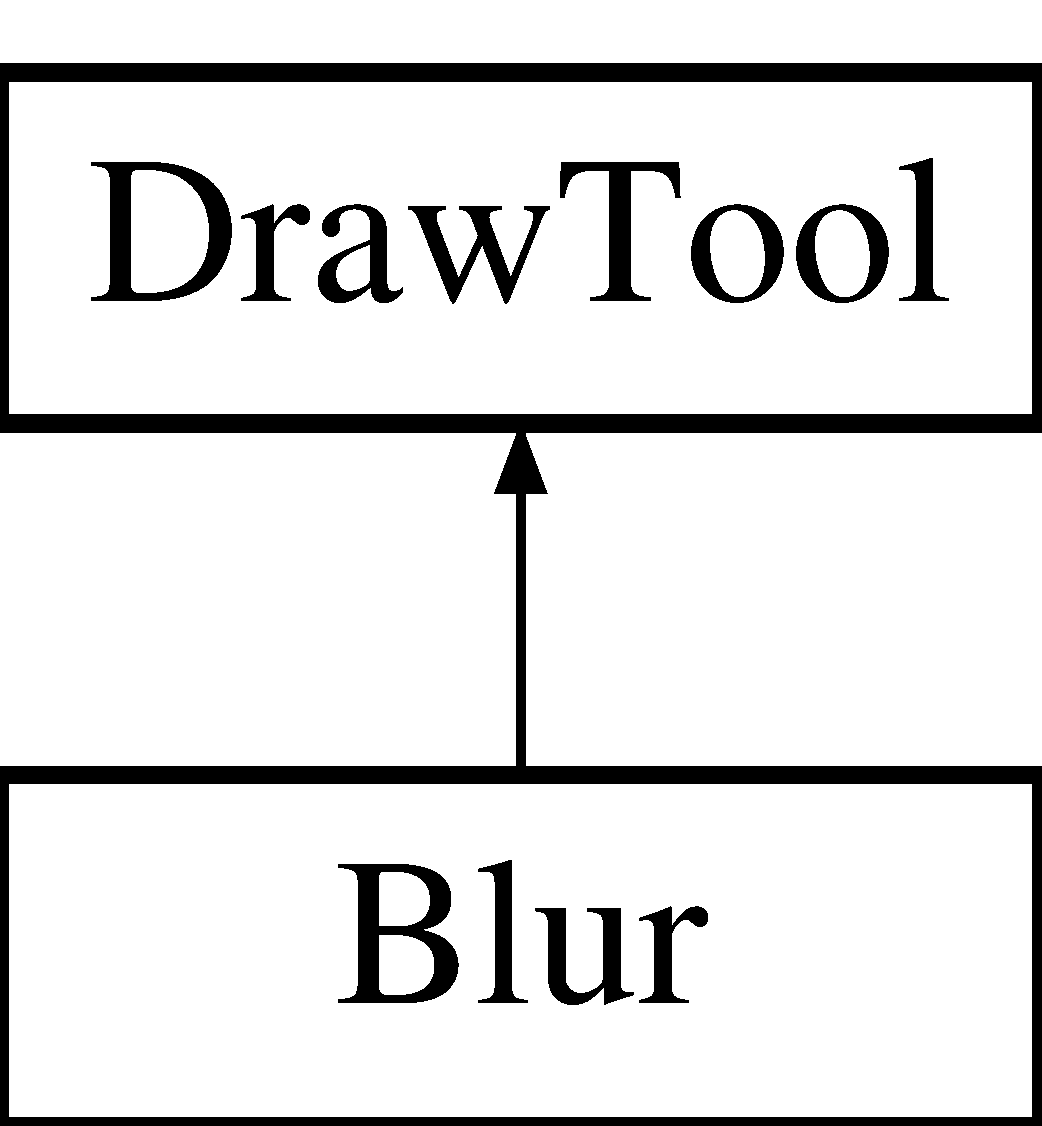
\includegraphics[height=2.000000cm]{classBlur}
\end{center}
\end{figure}
\subsection*{Public Member Functions}
\begin{DoxyCompactItemize}
\item 
\hyperlink{classBlur_a4cf976a139e3745e022c6b4fb7b18efb}{Blur} (int radius)
\item 
\hypertarget{classBlur_a6db41e9d70814abd7d188eee08779c7a}{void \hyperlink{classBlur_a6db41e9d70814abd7d188eee08779c7a}{fill\-Influence} ()}\label{classBlur_a6db41e9d70814abd7d188eee08779c7a}

\begin{DoxyCompactList}\small\item\em This creates a 2\-D matrix, the values at each index refer to the strength at which the color at that relative pixel should be applied. \end{DoxyCompactList}\item 
\hypertarget{classBlur_a74a6e5acef4b46edc5c79e909296ff53}{void \hyperlink{classBlur_a74a6e5acef4b46edc5c79e909296ff53}{apply\-Influence} (int x, int y, \hyperlink{classPixelBuffer}{Pixel\-Buffer} $\ast$buffer)}\label{classBlur_a74a6e5acef4b46edc5c79e909296ff53}

\begin{DoxyCompactList}\small\item\em This applies the influence matrix, the values at each index refer to the strength at which the color at that relative pixel should be applied. \end{DoxyCompactList}\item 
\hypertarget{classBlur_ad04ff612443d12024ae057ae757e6271}{string \hyperlink{classBlur_ad04ff612443d12024ae057ae757e6271}{get\-Name} ()}\label{classBlur_ad04ff612443d12024ae057ae757e6271}

\begin{DoxyCompactList}\small\item\em The publically viewable name the user sees. \end{DoxyCompactList}\end{DoxyCompactItemize}
\subsection*{Additional Inherited Members}


\subsection{Constructor \& Destructor Documentation}
\hypertarget{classBlur_a4cf976a139e3745e022c6b4fb7b18efb}{\index{Blur@{Blur}!Blur@{Blur}}
\index{Blur@{Blur}!Blur@{Blur}}
\subsubsection[{Blur}]{\setlength{\rightskip}{0pt plus 5cm}Blur\-::\-Blur (
\begin{DoxyParamCaption}
\item[{int}]{radius}
\end{DoxyParamCaption}
)}}\label{classBlur_a4cf976a139e3745e022c6b4fb7b18efb}
This is a base class that inherits from \hyperlink{classDrawTool}{Draw\-Tool}. This is used for the blur tool. 

The documentation for this class was generated from the following files\-:\begin{DoxyCompactItemize}
\item 
libphoto/Blur.\-h\item 
libphoto/Blur.\-cpp\end{DoxyCompactItemize}

\hypertarget{classCalligraphyPen}{\section{Calligraphy\-Pen Class Reference}
\label{classCalligraphyPen}\index{Calligraphy\-Pen@{Calligraphy\-Pen}}
}
Inheritance diagram for Calligraphy\-Pen\-:\begin{figure}[H]
\begin{center}
\leavevmode
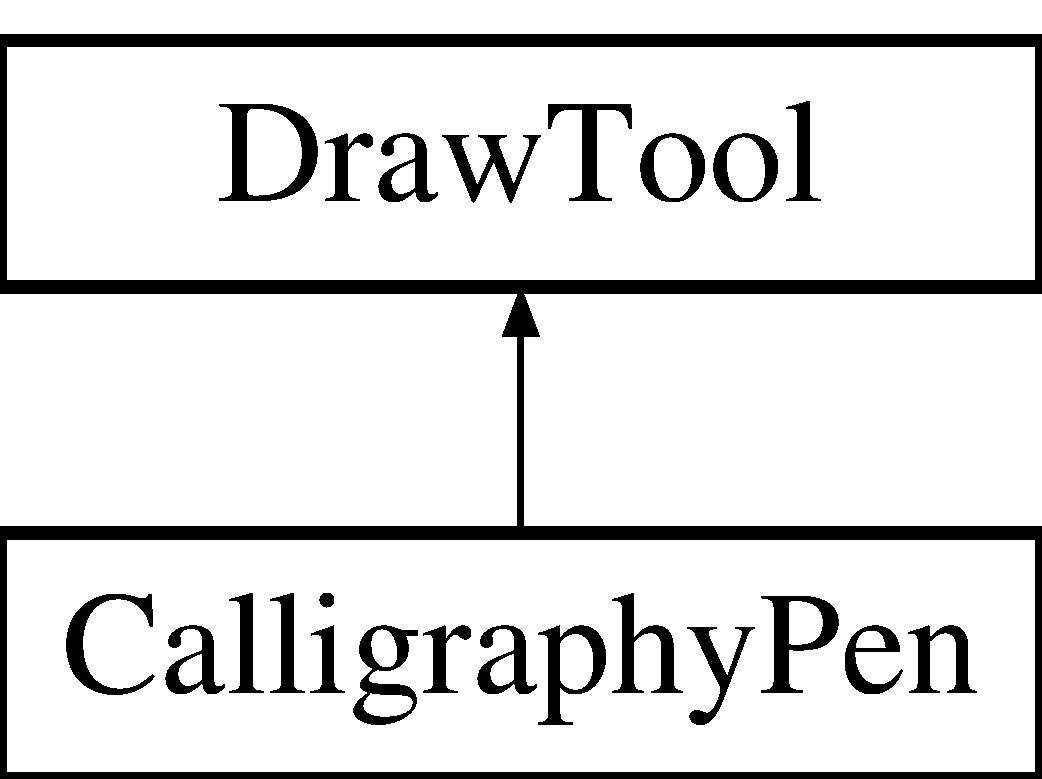
\includegraphics[height=2.000000cm]{classCalligraphyPen}
\end{center}
\end{figure}
\subsection*{Public Member Functions}
\begin{DoxyCompactItemize}
\item 
\hypertarget{classCalligraphyPen_a0a7aee1d27a037b4d863df7433530e54}{{\bfseries Calligraphy\-Pen} (\hyperlink{classColorData}{Color\-Data} $\ast$tool\-Color, int height, int width)}\label{classCalligraphyPen_a0a7aee1d27a037b4d863df7433530e54}

\item 
\hypertarget{classCalligraphyPen_add13526712abc99aad6cac69274d35ef}{void {\bfseries fill\-Influence} ()}\label{classCalligraphyPen_add13526712abc99aad6cac69274d35ef}

\item 
\hypertarget{classCalligraphyPen_a0a7aee1d27a037b4d863df7433530e54}{{\bfseries Calligraphy\-Pen} (\hyperlink{classColorData}{Color\-Data} $\ast$tool\-Color, int height, int width)}\label{classCalligraphyPen_a0a7aee1d27a037b4d863df7433530e54}

\item 
\hypertarget{classCalligraphyPen_add13526712abc99aad6cac69274d35ef}{void {\bfseries fill\-Influence} ()}\label{classCalligraphyPen_add13526712abc99aad6cac69274d35ef}

\item 
\hypertarget{classCalligraphyPen_a0a7aee1d27a037b4d863df7433530e54}{{\bfseries Calligraphy\-Pen} (\hyperlink{classColorData}{Color\-Data} $\ast$tool\-Color, int height, int width)}\label{classCalligraphyPen_a0a7aee1d27a037b4d863df7433530e54}

\item 
\hypertarget{classCalligraphyPen_add13526712abc99aad6cac69274d35ef}{void {\bfseries fill\-Influence} ()}\label{classCalligraphyPen_add13526712abc99aad6cac69274d35ef}

\end{DoxyCompactItemize}
\subsection*{Additional Inherited Members}


The documentation for this class was generated from the following files\-:\begin{DoxyCompactItemize}
\item 
libphoto/Calligraphy\-Pen.\-h\item 
libphoto/include/libphoto.\-h\item 
libphoto/Calligraphy\-Pen.\-cpp\end{DoxyCompactItemize}

\hypertarget{classColorData}{\section{Color\-Data Class Reference}
\label{classColorData}\index{Color\-Data@{Color\-Data}}
}


{\ttfamily \#include $<$Color\-Data.\-h$>$}

\subsection*{Public Member Functions}
\begin{DoxyCompactItemize}
\item 
\hyperlink{classColorData_accf4e0c0d4549051a46783e964c95164}{Color\-Data} ()
\item 
\hypertarget{classColorData_a920b0332685ef72147fe19020fdac5d6}{{\bfseries Color\-Data} (float r, float g, float b)}\label{classColorData_a920b0332685ef72147fe19020fdac5d6}

\item 
\hypertarget{classColorData_a0ecce2c6c597d9379ebb329883298dfd}{{\bfseries Color\-Data} (float r, float g, float b, float a)}\label{classColorData_a0ecce2c6c597d9379ebb329883298dfd}

\item 
\hypertarget{classColorData_aa2e401956936f87a560b8f579514bf69}{void \hyperlink{classColorData_aa2e401956936f87a560b8f579514bf69}{set\-Red} (float r)}\label{classColorData_aa2e401956936f87a560b8f579514bf69}

\begin{DoxyCompactList}\small\item\em Set the red value of the current object. \end{DoxyCompactList}\item 
\hypertarget{classColorData_a01bbba90cac0bc1b3bd01d4aecc16477}{void \hyperlink{classColorData_a01bbba90cac0bc1b3bd01d4aecc16477}{set\-Blue} (float b)}\label{classColorData_a01bbba90cac0bc1b3bd01d4aecc16477}

\begin{DoxyCompactList}\small\item\em Set the blue value of the current object. \end{DoxyCompactList}\item 
\hypertarget{classColorData_a4a7833dfef4a33eee3857de09a72aee1}{void \hyperlink{classColorData_a4a7833dfef4a33eee3857de09a72aee1}{set\-Green} (float g)}\label{classColorData_a4a7833dfef4a33eee3857de09a72aee1}

\begin{DoxyCompactList}\small\item\em Set the green value of the current object. \end{DoxyCompactList}\item 
\hypertarget{classColorData_a547fb7bd1616e8657a825cb9a34c43c1}{void \hyperlink{classColorData_a547fb7bd1616e8657a825cb9a34c43c1}{set\-Alpha} (float a)}\label{classColorData_a547fb7bd1616e8657a825cb9a34c43c1}

\begin{DoxyCompactList}\small\item\em Set the alpha value of the current object. \end{DoxyCompactList}\item 
\hypertarget{classColorData_ab7066467c08dfad868fc4b1add70c2f2}{float \hyperlink{classColorData_ab7066467c08dfad868fc4b1add70c2f2}{get\-Red} () const }\label{classColorData_ab7066467c08dfad868fc4b1add70c2f2}

\begin{DoxyCompactList}\small\item\em Get the red value of the current object. \end{DoxyCompactList}\item 
\hypertarget{classColorData_ad9c600256c8abefdd76209fc1f68fcb5}{float \hyperlink{classColorData_ad9c600256c8abefdd76209fc1f68fcb5}{get\-Blue} () const }\label{classColorData_ad9c600256c8abefdd76209fc1f68fcb5}

\begin{DoxyCompactList}\small\item\em Get the blue value of the current object. \end{DoxyCompactList}\item 
\hypertarget{classColorData_a7e2e03b8e1e3270f33c4e4a69c00dbd6}{float \hyperlink{classColorData_a7e2e03b8e1e3270f33c4e4a69c00dbd6}{get\-Green} () const }\label{classColorData_a7e2e03b8e1e3270f33c4e4a69c00dbd6}

\begin{DoxyCompactList}\small\item\em Get the green value of the current object. \end{DoxyCompactList}\item 
\hypertarget{classColorData_a198c4490b4f1c512d2bc174418dc892a}{float {\bfseries get\-Alpha} () const }\label{classColorData_a198c4490b4f1c512d2bc174418dc892a}

\item 
\hypertarget{classColorData_ae6a0100e4e5fe7bbd00fb4defd6e4a43}{float {\bfseries get\-Luminance} () const }\label{classColorData_ae6a0100e4e5fe7bbd00fb4defd6e4a43}

\item 
\hypertarget{classColorData_a3f0f9e50c730eb653efd800070cf448c}{float {\bfseries get\-Color\-Sum} () const }\label{classColorData_a3f0f9e50c730eb653efd800070cf448c}

\item 
\hypertarget{classColorData_a5479f50514f714dc9c738a50b7b86365}{\hyperlink{classColorData}{Color\-Data} {\bfseries clamped\-Color} () const }\label{classColorData_a5479f50514f714dc9c738a50b7b86365}

\end{DoxyCompactItemize}
\subsection*{Static Private Member Functions}
\begin{DoxyCompactItemize}
\item 
\hypertarget{classColorData_a2e6ef72b4053a043ac66f3c53556b89c}{static float {\bfseries clamp\-Value} (float input, float a, float b)}\label{classColorData_a2e6ef72b4053a043ac66f3c53556b89c}

\end{DoxyCompactItemize}
\subsection*{Private Attributes}
\begin{DoxyCompactItemize}
\item 
\hypertarget{classColorData_ab085dd5021fee2698e03baf20d89bfc4}{float {\bfseries m\-\_\-red}}\label{classColorData_ab085dd5021fee2698e03baf20d89bfc4}

\item 
\hypertarget{classColorData_a594f89816d552a2cfcb91fe0ce8df2ce}{float {\bfseries m\-\_\-green}}\label{classColorData_a594f89816d552a2cfcb91fe0ce8df2ce}

\item 
\hypertarget{classColorData_a811102de4cfed5429beedcc67714520f}{float {\bfseries m\-\_\-blue}}\label{classColorData_a811102de4cfed5429beedcc67714520f}

\item 
\hypertarget{classColorData_ae8318f47f7ba2a9e2fd70b7dd03ef672}{float {\bfseries m\-\_\-alpha}}\label{classColorData_ae8318f47f7ba2a9e2fd70b7dd03ef672}

\end{DoxyCompactItemize}
\subsection*{Friends}
\begin{DoxyCompactItemize}
\item 
\hypertarget{classColorData_adf9a770243996e50282d248a4327f351}{\hyperlink{classColorData}{Color\-Data} \hyperlink{classColorData_adf9a770243996e50282d248a4327f351}{operator$\ast$} (const \hyperlink{classColorData}{Color\-Data} \&a, float f)}\label{classColorData_adf9a770243996e50282d248a4327f351}

\begin{DoxyCompactList}\small\item\em Apply component-\/wise arithmatic operations. \end{DoxyCompactList}\item 
\hypertarget{classColorData_afdc3e8e6338798779739352e6bdfa42b}{\hyperlink{classColorData}{Color\-Data} {\bfseries operator$\ast$} (const \hyperlink{classColorData}{Color\-Data} \&a, const \hyperlink{classColorData}{Color\-Data} \&b)}\label{classColorData_afdc3e8e6338798779739352e6bdfa42b}

\item 
\hypertarget{classColorData_afee00faf26189979b72f3854a17200ae}{\hyperlink{classColorData}{Color\-Data} {\bfseries operator+} (const \hyperlink{classColorData}{Color\-Data} \&a, const \hyperlink{classColorData}{Color\-Data} \&b)}\label{classColorData_afee00faf26189979b72f3854a17200ae}

\item 
\hypertarget{classColorData_a799bd54f65a61569b5b968062ac0d37e}{\hyperlink{classColorData}{Color\-Data} {\bfseries operator-\/} (const \hyperlink{classColorData}{Color\-Data} \&a, const \hyperlink{classColorData}{Color\-Data} \&b)}\label{classColorData_a799bd54f65a61569b5b968062ac0d37e}

\item 
\hypertarget{classColorData_a9dae9e77610393d100312c9d248f09cc}{bool {\bfseries operator==} (const \hyperlink{classColorData}{Color\-Data} \&a, const \hyperlink{classColorData}{Color\-Data} \&b)}\label{classColorData_a9dae9e77610393d100312c9d248f09cc}

\item 
\hypertarget{classColorData_a698ac263a286afe37e3b9ed0c5882c8c}{bool {\bfseries operator!=} (const \hyperlink{classColorData}{Color\-Data} \&a, const \hyperlink{classColorData}{Color\-Data} \&b)}\label{classColorData_a698ac263a286afe37e3b9ed0c5882c8c}

\end{DoxyCompactItemize}


\subsection{Detailed Description}
This color data class stores color in floating point format. The Red, Green, Blue, and Alpha channels range from 0.\-0 to 1.\-0. 

\subsection{Constructor \& Destructor Documentation}
\hypertarget{classColorData_accf4e0c0d4549051a46783e964c95164}{\index{Color\-Data@{Color\-Data}!Color\-Data@{Color\-Data}}
\index{Color\-Data@{Color\-Data}!ColorData@{Color\-Data}}
\subsubsection[{Color\-Data}]{\setlength{\rightskip}{0pt plus 5cm}Color\-Data\-::\-Color\-Data (
\begin{DoxyParamCaption}
{}
\end{DoxyParamCaption}
)}}\label{classColorData_accf4e0c0d4549051a46783e964c95164}
This is the color data class. Every pixel contains a colordata object detailing the r,g,b, and sometimes a values. 

The documentation for this class was generated from the following files\-:\begin{DoxyCompactItemize}
\item 
libphoto/Color\-Data.\-h\item 
libphoto/Color\-Data.\-cpp\end{DoxyCompactItemize}

\hypertarget{classCrayon}{\section{Crayon Class Reference}
\label{classCrayon}\index{Crayon@{Crayon}}
}
Inheritance diagram for Crayon\-:\begin{figure}[H]
\begin{center}
\leavevmode
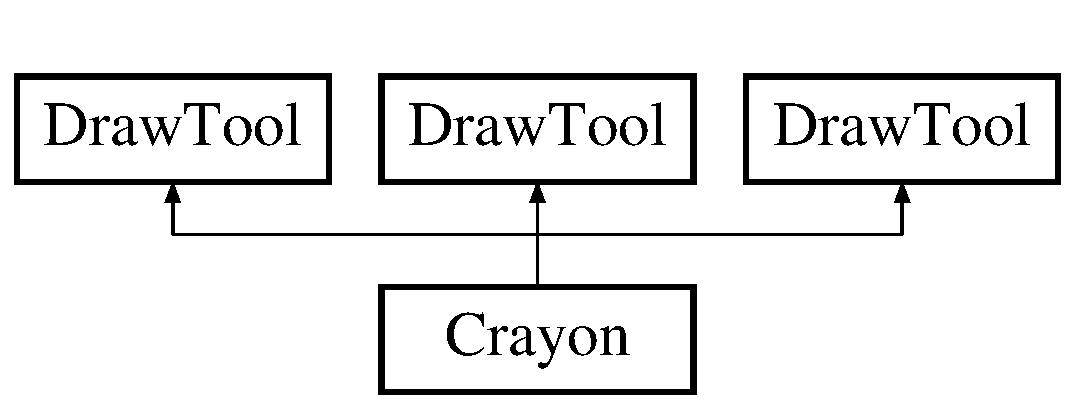
\includegraphics[height=2.000000cm]{classCrayon}
\end{center}
\end{figure}
\subsection*{Public Member Functions}
\begin{DoxyCompactItemize}
\item 
\hyperlink{classCrayon_a705e3468d3ede98a95f792bfd05be7dd}{Crayon} (\hyperlink{classColorData}{Color\-Data} $\ast$tool\-Color, int radius)
\begin{DoxyCompactList}\small\item\em For function descriptions please see the \hyperlink{classBlur}{Blur} class. \end{DoxyCompactList}\item 
void \hyperlink{classCrayon_a2af3bd14c6bc719a252a9c9f1c5eccb7}{fill\-Influence} ()
\item 
\hypertarget{classCrayon_a0484aec2b5ac3d6147e4e0bf8b3aa9d4}{string {\bfseries get\-Name} ()}\label{classCrayon_a0484aec2b5ac3d6147e4e0bf8b3aa9d4}

\end{DoxyCompactItemize}
\subsection*{Additional Inherited Members}


\subsection{Constructor \& Destructor Documentation}
\hypertarget{classCrayon_a705e3468d3ede98a95f792bfd05be7dd}{\index{Crayon@{Crayon}!Crayon@{Crayon}}
\index{Crayon@{Crayon}!Crayon@{Crayon}}
\subsubsection[{Crayon}]{\setlength{\rightskip}{0pt plus 5cm}Crayon\-::\-Crayon (
\begin{DoxyParamCaption}
\item[{{\bf Color\-Data} $\ast$}]{tool\-Color, }
\item[{int}]{radius}
\end{DoxyParamCaption}
)}}\label{classCrayon_a705e3468d3ede98a95f792bfd05be7dd}


For function descriptions please see the \hyperlink{classBlur}{Blur} class. 

This is the \hyperlink{classCrayon}{Crayon} pen class, it inherits from \hyperlink{classDrawTool}{Draw\-Tool} and is used for the \hyperlink{classCrayon}{Crayon} pen 

\subsection{Member Function Documentation}
\hypertarget{classCrayon_a2af3bd14c6bc719a252a9c9f1c5eccb7}{\index{Crayon@{Crayon}!fill\-Influence@{fill\-Influence}}
\index{fill\-Influence@{fill\-Influence}!Crayon@{Crayon}}
\subsubsection[{fill\-Influence}]{\setlength{\rightskip}{0pt plus 5cm}void Crayon\-::fill\-Influence (
\begin{DoxyParamCaption}
{}
\end{DoxyParamCaption}
)\hspace{0.3cm}{\ttfamily [virtual]}}}\label{classCrayon_a2af3bd14c6bc719a252a9c9f1c5eccb7}
Virtual function to set influence on the mask, should be overrode in sub class \par
 none \par
 void \par


Reimplemented from \hyperlink{classDrawTool_ae202bc193ba721452e81f34b6c2e6e35}{Draw\-Tool}.



The documentation for this class was generated from the following files\-:\begin{DoxyCompactItemize}
\item 
libphoto/Crayon.\-h\item 
libphoto/Crayon.\-cpp\end{DoxyCompactItemize}

\hypertarget{classDrawTool}{\section{Draw\-Tool Class Reference}
\label{classDrawTool}\index{Draw\-Tool@{Draw\-Tool}}
}
Inheritance diagram for Draw\-Tool\-:\begin{figure}[H]
\begin{center}
\leavevmode
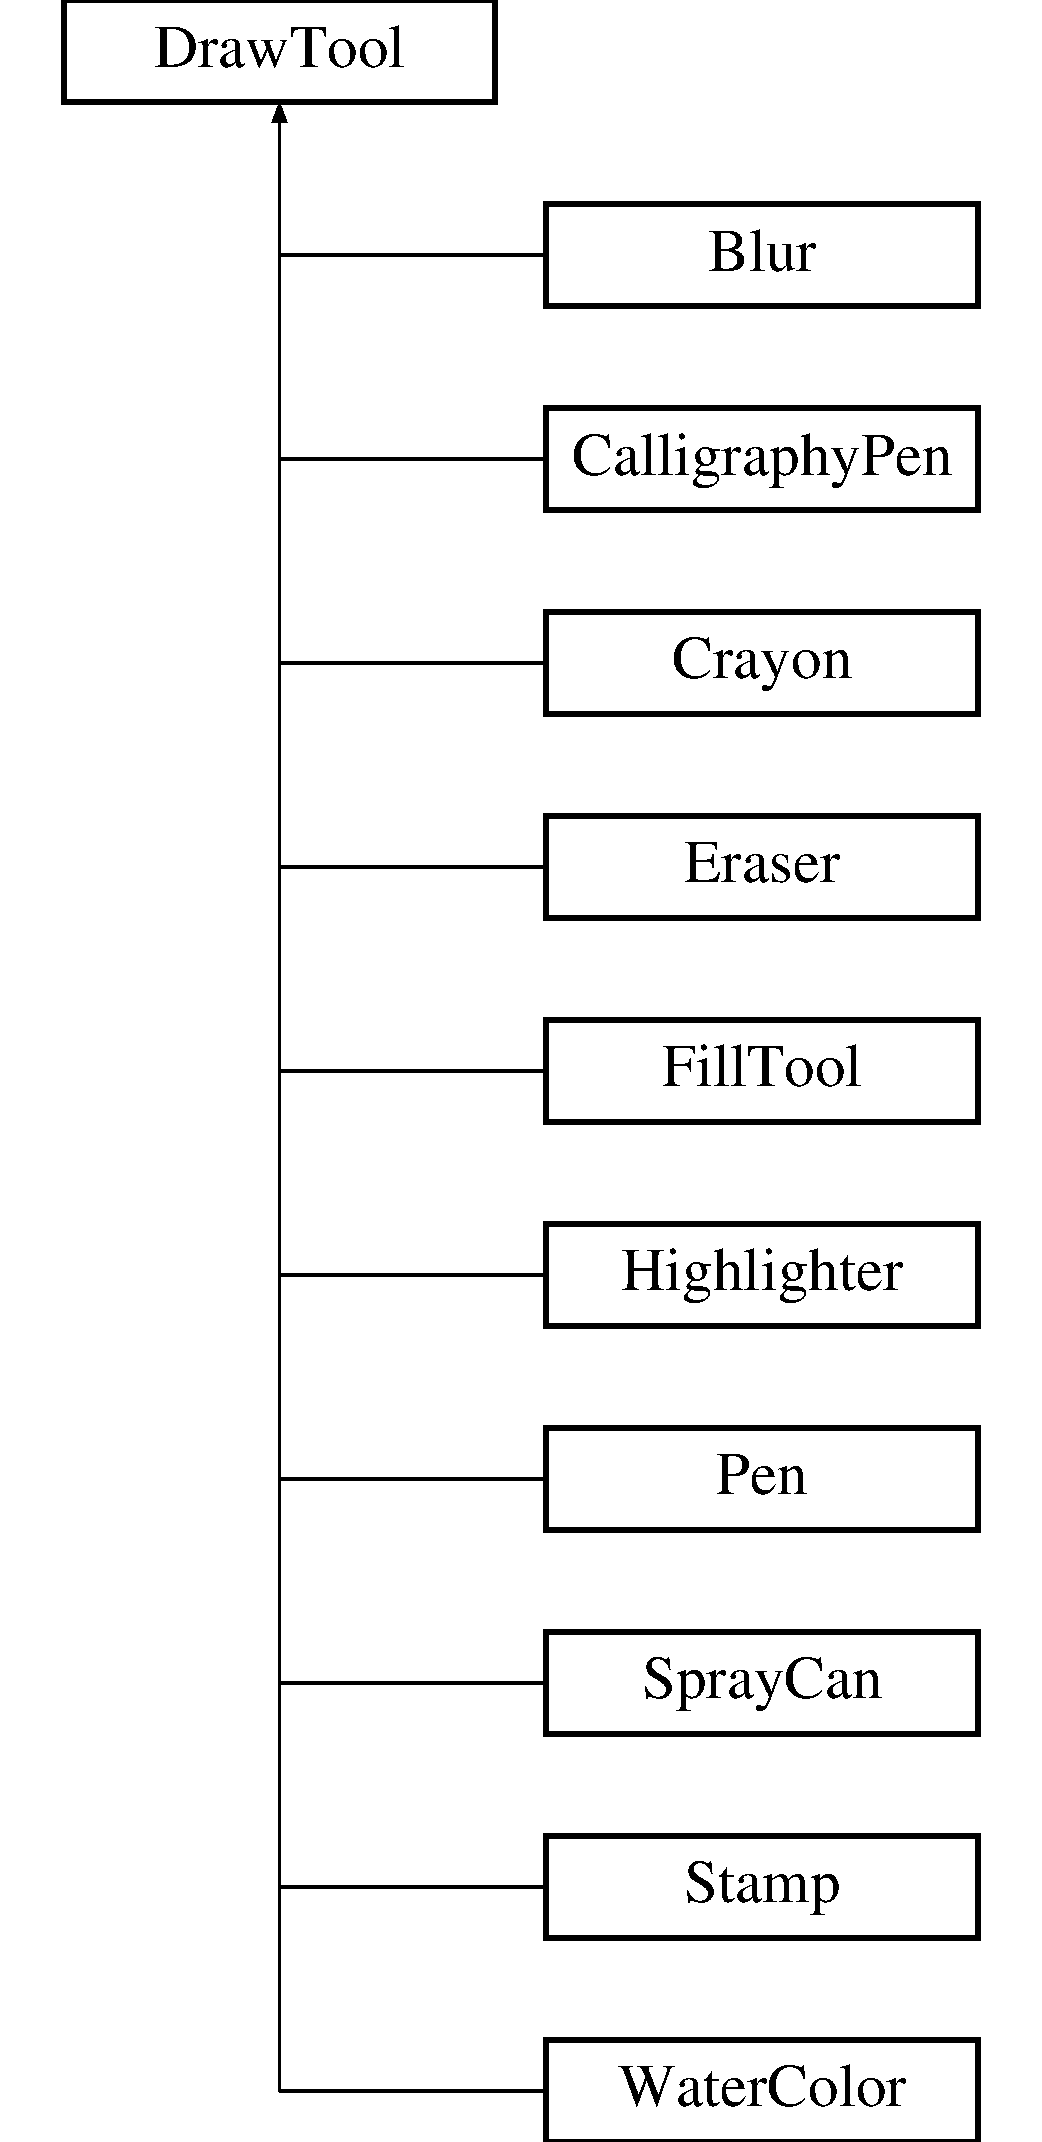
\includegraphics[height=11.000000cm]{classDrawTool}
\end{center}
\end{figure}
\subsection*{Public Member Functions}
\begin{DoxyCompactItemize}
\item 
\hypertarget{classDrawTool_aa21e3a5373ba9e4e43d6e56eec82b32d}{{\bfseries Draw\-Tool} (\hyperlink{classColorData}{Color\-Data} $\ast$tool\-Color, int width, int height)}\label{classDrawTool_aa21e3a5373ba9e4e43d6e56eec82b32d}

\item 
\hypertarget{classDrawTool_aa1816d6699a835d9c7619ee5c97be9d1}{{\bfseries Draw\-Tool} (int width, int height)}\label{classDrawTool_aa1816d6699a835d9c7619ee5c97be9d1}

\item 
\hypertarget{classDrawTool_a521ad2f183dd3354de1dd163140e8b1d}{{\bfseries Draw\-Tool} (\hyperlink{classPixelBuffer}{Pixel\-Buffer} $\ast$new\-Buffer, int width, int height)}\label{classDrawTool_a521ad2f183dd3354de1dd163140e8b1d}

\item 
\hypertarget{classDrawTool_ae202bc193ba721452e81f34b6c2e6e35}{virtual void {\bfseries fill\-Influence} ()}\label{classDrawTool_ae202bc193ba721452e81f34b6c2e6e35}

\item 
\hypertarget{classDrawTool_a65dbb2f006efc9c6053d01df75eff5a9}{virtual void {\bfseries paint} (int x, int y, int prev\-X, int prev\-Y, \hyperlink{classPixelBuffer}{Pixel\-Buffer} $\ast$buffer)}\label{classDrawTool_a65dbb2f006efc9c6053d01df75eff5a9}

\item 
\hypertarget{classDrawTool_ac60a70d91e81163d413b99382ac4255b}{virtual void {\bfseries apply\-Influence} (int x, int y, \hyperlink{classPixelBuffer}{Pixel\-Buffer} $\ast$buffer)}\label{classDrawTool_ac60a70d91e81163d413b99382ac4255b}

\item 
\hypertarget{classDrawTool_a11a450d969098c86158b6ec5f14d291e}{virtual string {\bfseries get\-Name} ()}\label{classDrawTool_a11a450d969098c86158b6ec5f14d291e}

\item 
\hypertarget{classDrawTool_ad11d4e44fcd2caf774e18ce5b2986865}{\hyperlink{classMask}{Mask} const $\ast$ {\bfseries get\-Mask} () const }\label{classDrawTool_ad11d4e44fcd2caf774e18ce5b2986865}

\item 
\hypertarget{classDrawTool_a00485271784acd5acc75840a7a17eb2e}{\hyperlink{classColorData}{Color\-Data} const $\ast$ {\bfseries get\-Tool\-Color} () const }\label{classDrawTool_a00485271784acd5acc75840a7a17eb2e}

\item 
\hypertarget{classDrawTool_a7f7097be5f6beb7b3f6ce437785cac7a}{void {\bfseries set\-Tool\-Color} (\hyperlink{classColorData}{Color\-Data} $\ast$color)}\label{classDrawTool_a7f7097be5f6beb7b3f6ce437785cac7a}

\item 
\hypertarget{classDrawTool_a04f57381cb6c71d90a66e905b46f424c}{void {\bfseries printf\-Influence} ()}\label{classDrawTool_a04f57381cb6c71d90a66e905b46f424c}

\end{DoxyCompactItemize}
\subsection*{Public Attributes}
\begin{DoxyCompactItemize}
\item 
\hypertarget{classDrawTool_a87f991a7c84a4c5ad60ebbfd813a3ab2}{bool {\bfseries allow\-Drag}}\label{classDrawTool_a87f991a7c84a4c5ad60ebbfd813a3ab2}

\end{DoxyCompactItemize}
\subsection*{Protected Attributes}
\begin{DoxyCompactItemize}
\item 
\hypertarget{classDrawTool_a0a3cc5165047f1158bff38750ddf8e85}{\hyperlink{classMask}{Mask} $\ast$ {\bfseries m\-\_\-mask}}\label{classDrawTool_a0a3cc5165047f1158bff38750ddf8e85}

\item 
\hypertarget{classDrawTool_a3bb9153560d2b084c56d5e7d749d49a2}{\hyperlink{classColorData}{Color\-Data} $\ast$ {\bfseries m\-\_\-tool\-Color}}\label{classDrawTool_a3bb9153560d2b084c56d5e7d749d49a2}

\item 
\hypertarget{classDrawTool_a917dfe1261ea0d5c4250f8b83eddb177}{\hyperlink{classPixelBuffer}{Pixel\-Buffer} $\ast$ {\bfseries image\-Buffer}}\label{classDrawTool_a917dfe1261ea0d5c4250f8b83eddb177}

\end{DoxyCompactItemize}


The documentation for this class was generated from the following files\-:\begin{DoxyCompactItemize}
\item 
libphoto/Drawtool.\-h\item 
libphoto/Drawtool.\-cpp\end{DoxyCompactItemize}

\hypertarget{classEraser}{\section{Eraser Class Reference}
\label{classEraser}\index{Eraser@{Eraser}}
}
Inheritance diagram for Eraser\-:\begin{figure}[H]
\begin{center}
\leavevmode
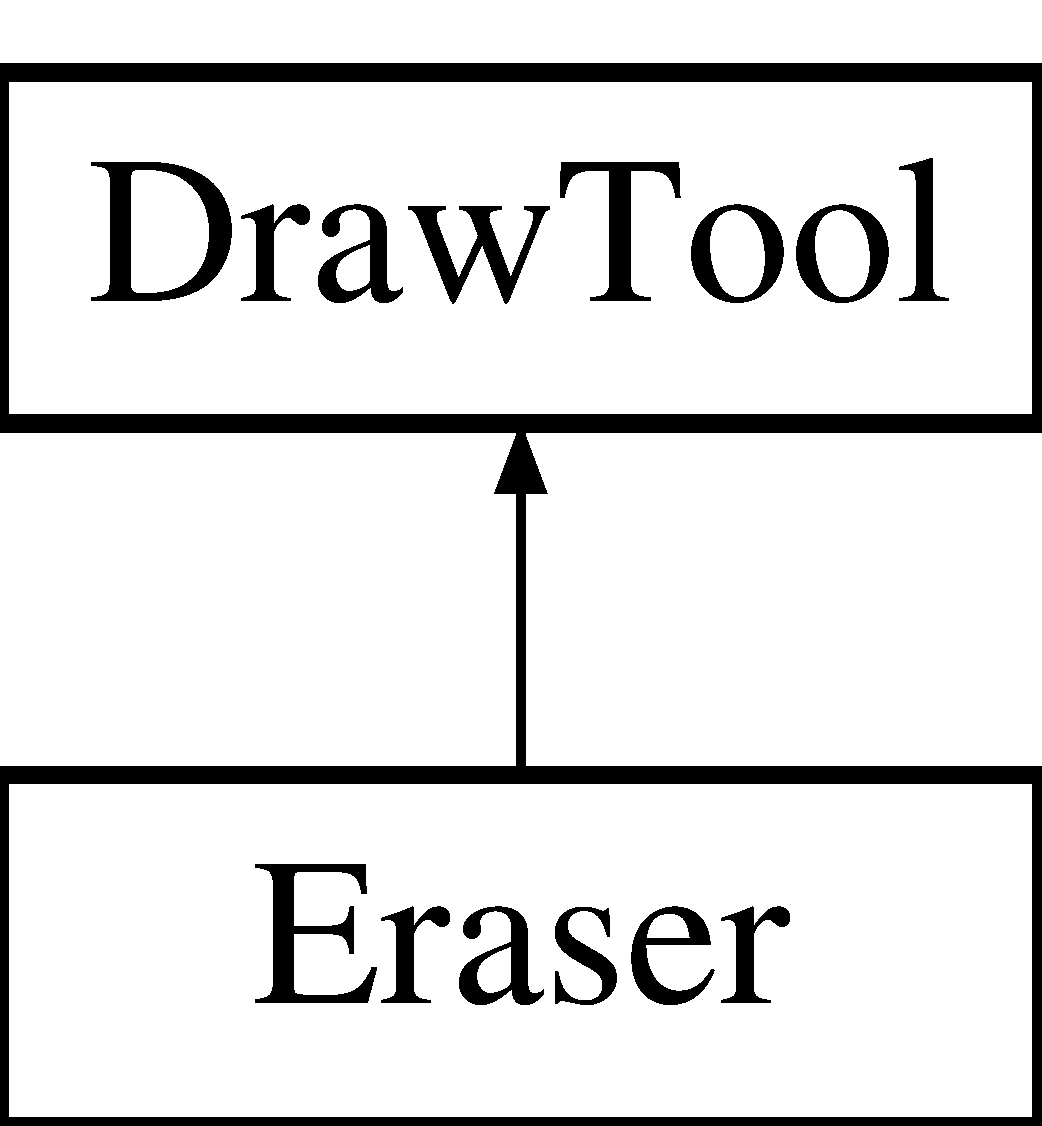
\includegraphics[height=2.000000cm]{classEraser}
\end{center}
\end{figure}
\subsection*{Public Member Functions}
\begin{DoxyCompactItemize}
\item 
\hypertarget{classEraser_a60abccb4522452a4cdfb714eafbc9c16}{{\bfseries Eraser} (int radius)}\label{classEraser_a60abccb4522452a4cdfb714eafbc9c16}

\item 
\hypertarget{classEraser_a195eeec6843317ee33e0e51fccb3daff}{void {\bfseries apply\-Influence} (int x, int y, \hyperlink{classPixelBuffer}{Pixel\-Buffer} $\ast$buffer)}\label{classEraser_a195eeec6843317ee33e0e51fccb3daff}

\item 
\hypertarget{classEraser_ad718ebd5796e0a83dbd94aa4f0ce2921}{void {\bfseries fill\-Influence} ()}\label{classEraser_ad718ebd5796e0a83dbd94aa4f0ce2921}

\item 
\hypertarget{classEraser_a60abccb4522452a4cdfb714eafbc9c16}{{\bfseries Eraser} (int radius)}\label{classEraser_a60abccb4522452a4cdfb714eafbc9c16}

\item 
\hypertarget{classEraser_a195eeec6843317ee33e0e51fccb3daff}{void {\bfseries apply\-Influence} (int x, int y, \hyperlink{classPixelBuffer}{Pixel\-Buffer} $\ast$buffer)}\label{classEraser_a195eeec6843317ee33e0e51fccb3daff}

\item 
\hypertarget{classEraser_ad718ebd5796e0a83dbd94aa4f0ce2921}{void {\bfseries fill\-Influence} ()}\label{classEraser_ad718ebd5796e0a83dbd94aa4f0ce2921}

\item 
\hypertarget{classEraser_a60abccb4522452a4cdfb714eafbc9c16}{{\bfseries Eraser} (int radius)}\label{classEraser_a60abccb4522452a4cdfb714eafbc9c16}

\item 
\hypertarget{classEraser_a195eeec6843317ee33e0e51fccb3daff}{void {\bfseries apply\-Influence} (int x, int y, \hyperlink{classPixelBuffer}{Pixel\-Buffer} $\ast$buffer)}\label{classEraser_a195eeec6843317ee33e0e51fccb3daff}

\item 
\hypertarget{classEraser_ad718ebd5796e0a83dbd94aa4f0ce2921}{void {\bfseries fill\-Influence} ()}\label{classEraser_ad718ebd5796e0a83dbd94aa4f0ce2921}

\end{DoxyCompactItemize}
\subsection*{Additional Inherited Members}


The documentation for this class was generated from the following files\-:\begin{DoxyCompactItemize}
\item 
libphoto/Eraser.\-h\item 
libphoto/include/libphoto.\-h\item 
libphoto/Eraser.\-cpp\end{DoxyCompactItemize}

\hypertarget{classFBlur}{\section{F\-Blur Class Reference}
\label{classFBlur}\index{F\-Blur@{F\-Blur}}
}
Inheritance diagram for F\-Blur\-:\begin{figure}[H]
\begin{center}
\leavevmode
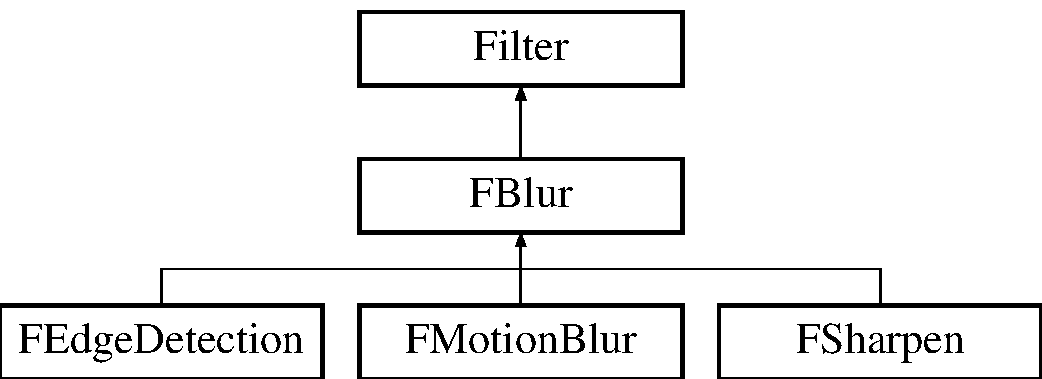
\includegraphics[height=3.000000cm]{classFBlur}
\end{center}
\end{figure}
\subsection*{Public Member Functions}
\begin{DoxyCompactItemize}
\item 
\hypertarget{classFBlur_a20d9f9bb8f2b787273a860779853a8fd}{void {\bfseries apply\-Filter} (\hyperlink{classPixelBuffer}{Pixel\-Buffer} $\ast$image\-Buffer)}\label{classFBlur_a20d9f9bb8f2b787273a860779853a8fd}

\item 
\hypertarget{classFBlur_a3c121581f48e00e0267f88826808ee23}{std\-::string {\bfseries get\-Name} ()}\label{classFBlur_a3c121581f48e00e0267f88826808ee23}

\item 
\hypertarget{classFBlur_ad7d9aa0fa6b3b4f4ead1545ccf6a6628}{virtual kernel\-Type {\bfseries build\-Kernel} (int radius)}\label{classFBlur_ad7d9aa0fa6b3b4f4ead1545ccf6a6628}

\item 
\hypertarget{classFBlur_a97ca2bede17042bae70d781859d46e73}{kernel\-Type {\bfseries box\-Filter} (int radius)}\label{classFBlur_a97ca2bede17042bae70d781859d46e73}

\item 
\hypertarget{classFBlur_ab13f7d8c36423e3f0ecabdcd9b045fbf}{kernel\-Type {\bfseries empty\-Filter} (int radius)}\label{classFBlur_ab13f7d8c36423e3f0ecabdcd9b045fbf}

\item 
\hypertarget{classFBlur_ad88afc728cb9b8c84443a0bf4a30983f}{kernel\-Type {\bfseries Gaussian\-Blur} (float sigma)}\label{classFBlur_ad88afc728cb9b8c84443a0bf4a30983f}

\item 
\hypertarget{classFBlur_a7cb16fe19cd319be83d95de5686e8d39}{kernel\-Type {\bfseries get\-Kernel} ()}\label{classFBlur_a7cb16fe19cd319be83d95de5686e8d39}

\item 
\hypertarget{classFBlur_a5f500e9bad040039fb43e58be03d57e6}{void {\bfseries print\-Kernel} ()}\label{classFBlur_a5f500e9bad040039fb43e58be03d57e6}

\end{DoxyCompactItemize}


The documentation for this class was generated from the following files\-:\begin{DoxyCompactItemize}
\item 
libphoto/F\-Blur.\-h\item 
libphoto/F\-Blur.\-cpp\end{DoxyCompactItemize}

\hypertarget{classFChannel}{}\section{F\+Channel Class Reference}
\label{classFChannel}\index{F\+Channel@{F\+Channel}}
Inheritance diagram for F\+Channel\+:\begin{figure}[H]
\begin{center}
\leavevmode
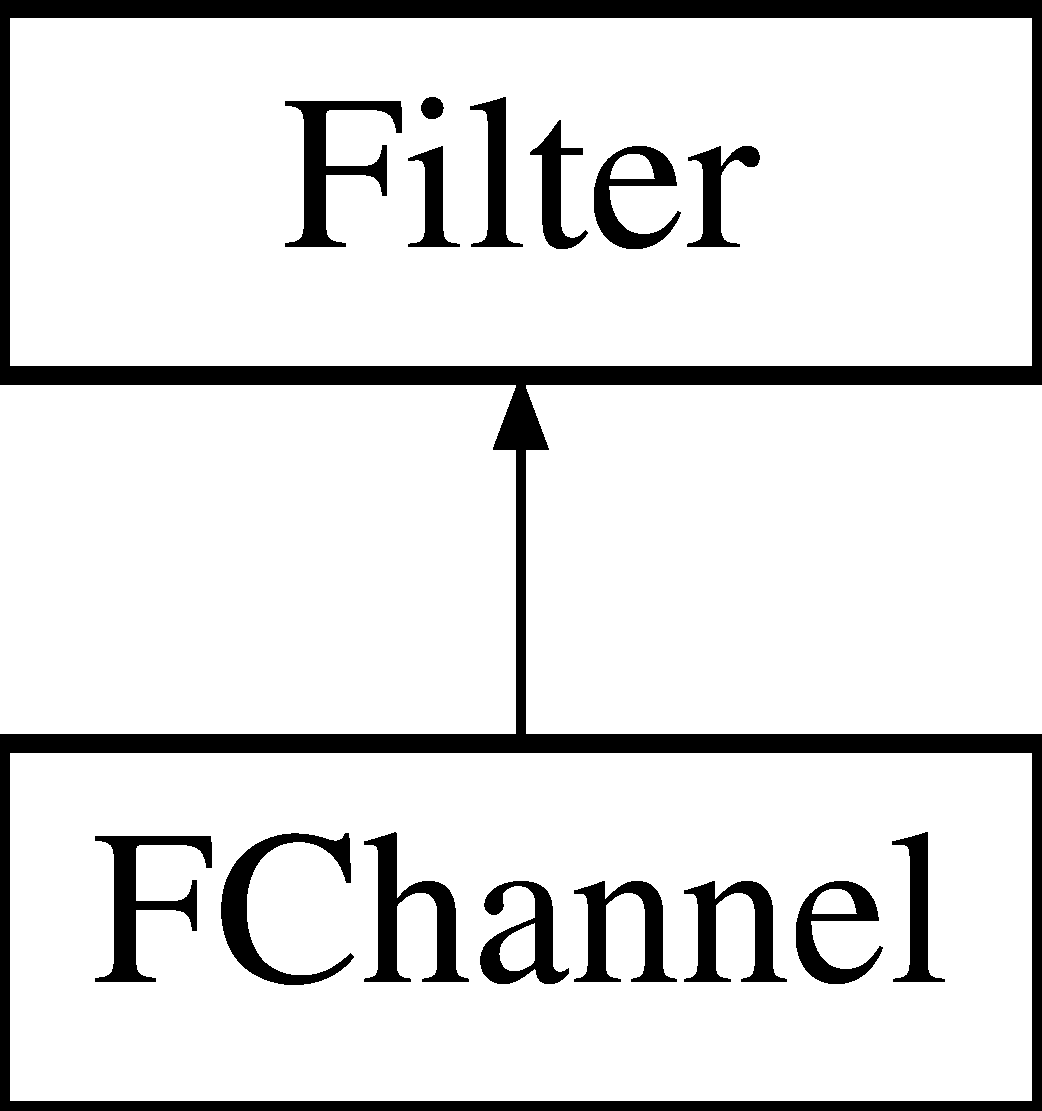
\includegraphics[height=2.000000cm]{classFChannel}
\end{center}
\end{figure}
\subsection*{Public Member Functions}
\begin{DoxyCompactItemize}
\item 
\hyperlink{classFChannel_acc91e001fcac19d758179c410e75be7a}{F\+Channel} ()
\item 
void \hyperlink{classFChannel_a74a786921c11b3d82119b74f05d3d0c0}{apply\+Filter} (\hyperlink{classPixelBuffer}{Pixel\+Buffer} $\ast$image\+Buffer)\hypertarget{classFChannel_a74a786921c11b3d82119b74f05d3d0c0}{}\label{classFChannel_a74a786921c11b3d82119b74f05d3d0c0}

\begin{DoxyCompactList}\small\item\em apply channel filter effect to the Pixel\+Buffer$\ast$ buffer passed into this function \end{DoxyCompactList}\item 
std\+::string \hyperlink{classFChannel_a3d7618565e8643f1a4f87d12a968e406}{get\+Name} ()\hypertarget{classFChannel_a3d7618565e8643f1a4f87d12a968e406}{}\label{classFChannel_a3d7618565e8643f1a4f87d12a968e406}

\begin{DoxyCompactList}\small\item\em get class name for filter \end{DoxyCompactList}\end{DoxyCompactItemize}


\subsection{Constructor \& Destructor Documentation}
\index{F\+Channel@{F\+Channel}!F\+Channel@{F\+Channel}}
\index{F\+Channel@{F\+Channel}!F\+Channel@{F\+Channel}}
\subsubsection[{\texorpdfstring{F\+Channel()}{FChannel()}}]{\setlength{\rightskip}{0pt plus 5cm}F\+Channel\+::\+F\+Channel (
\begin{DoxyParamCaption}
{}
\end{DoxyParamCaption}
)}\hypertarget{classFChannel_acc91e001fcac19d758179c410e75be7a}{}\label{classFChannel_acc91e001fcac19d758179c410e75be7a}
This is the \hyperlink{classFChannel}{F\+Channel} class, it is used for all the channel image filters . apply\+Filter describes how this filter will be applied to every pixel in the image. 

The documentation for this class was generated from the following files\+:\begin{DoxyCompactItemize}
\item 
libphoto/F\+Channel.\+h\item 
libphoto/F\+Channel.\+cpp\end{DoxyCompactItemize}

\hypertarget{classFEdgeDetection}{\section{F\-Edge\-Detection Class Reference}
\label{classFEdgeDetection}\index{F\-Edge\-Detection@{F\-Edge\-Detection}}
}
Inheritance diagram for F\-Edge\-Detection\-:\begin{figure}[H]
\begin{center}
\leavevmode
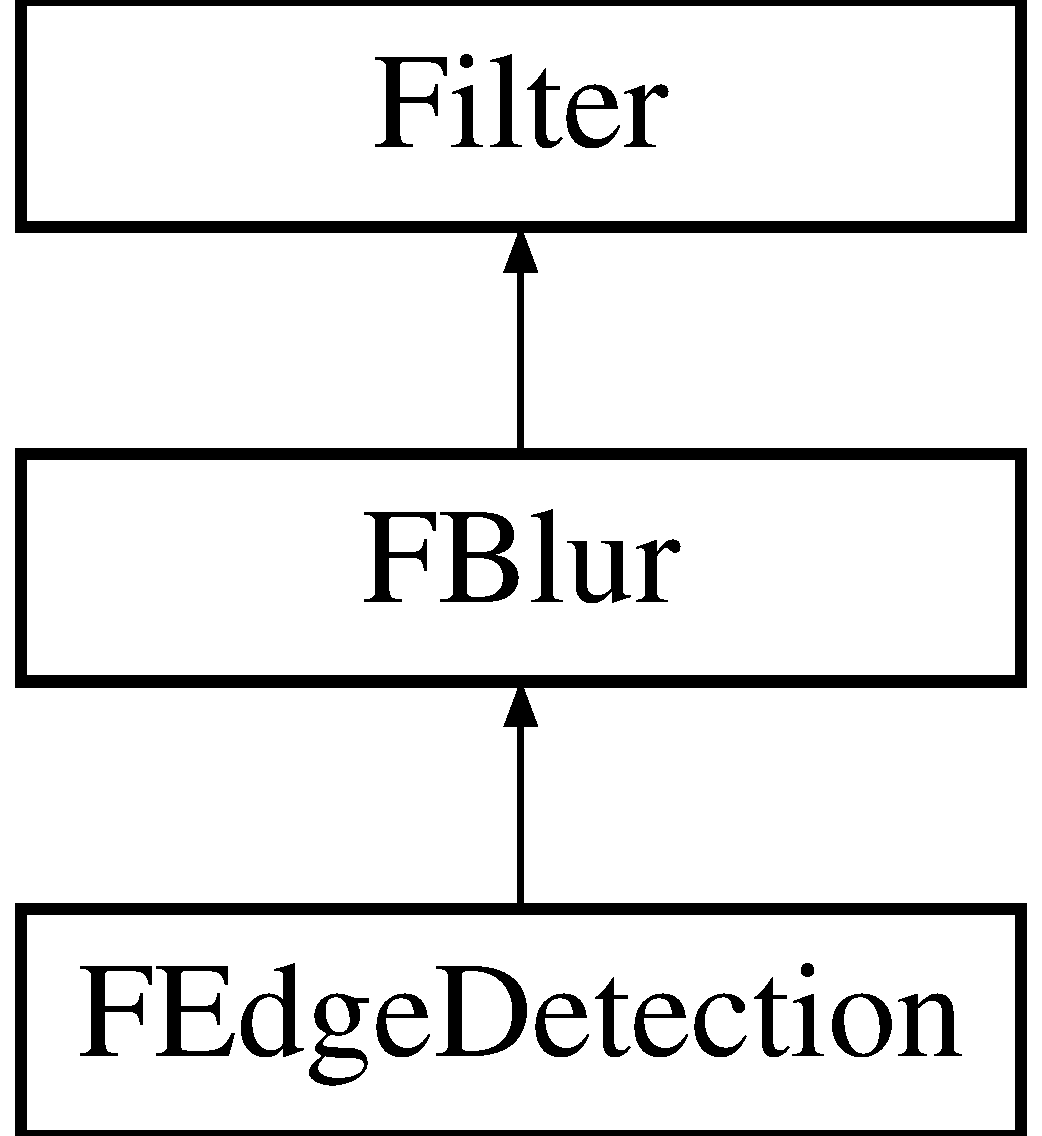
\includegraphics[height=4.242424cm]{classFEdgeDetection}
\end{center}
\end{figure}
\subsection*{Public Member Functions}
\begin{DoxyCompactItemize}
\item 
\hypertarget{classFEdgeDetection_acdf7ec56e2f1f5010b84ebcd66a958f3}{std\-::string {\bfseries get\-Name} ()}\label{classFEdgeDetection_acdf7ec56e2f1f5010b84ebcd66a958f3}

\item 
\hypertarget{classFEdgeDetection_a58c541bf60eb4e21bdb656bdad5f8c65}{kernel\-Type {\bfseries build\-Kernel} (int radius)}\label{classFEdgeDetection_a58c541bf60eb4e21bdb656bdad5f8c65}

\item 
\hypertarget{classFEdgeDetection_acdf7ec56e2f1f5010b84ebcd66a958f3}{std\-::string {\bfseries get\-Name} ()}\label{classFEdgeDetection_acdf7ec56e2f1f5010b84ebcd66a958f3}

\item 
\hypertarget{classFEdgeDetection_a58c541bf60eb4e21bdb656bdad5f8c65}{kernel\-Type {\bfseries build\-Kernel} (int radius)}\label{classFEdgeDetection_a58c541bf60eb4e21bdb656bdad5f8c65}

\item 
\hypertarget{classFEdgeDetection_acdf7ec56e2f1f5010b84ebcd66a958f3}{std\-::string {\bfseries get\-Name} ()}\label{classFEdgeDetection_acdf7ec56e2f1f5010b84ebcd66a958f3}

\item 
\hypertarget{classFEdgeDetection_a58c541bf60eb4e21bdb656bdad5f8c65}{kernel\-Type {\bfseries build\-Kernel} (int radius)}\label{classFEdgeDetection_a58c541bf60eb4e21bdb656bdad5f8c65}

\end{DoxyCompactItemize}
\subsection*{Additional Inherited Members}


The documentation for this class was generated from the following files\-:\begin{DoxyCompactItemize}
\item 
libphoto/F\-Edge\-Detection.\-h\item 
libphoto/include/libphoto.\-h\item 
libphoto/F\-Edge\-Detection.\-cpp\end{DoxyCompactItemize}

\hypertarget{classFillTool}{\section{Fill\-Tool Class Reference}
\label{classFillTool}\index{Fill\-Tool@{Fill\-Tool}}
}
Inheritance diagram for Fill\-Tool\-:\begin{figure}[H]
\begin{center}
\leavevmode
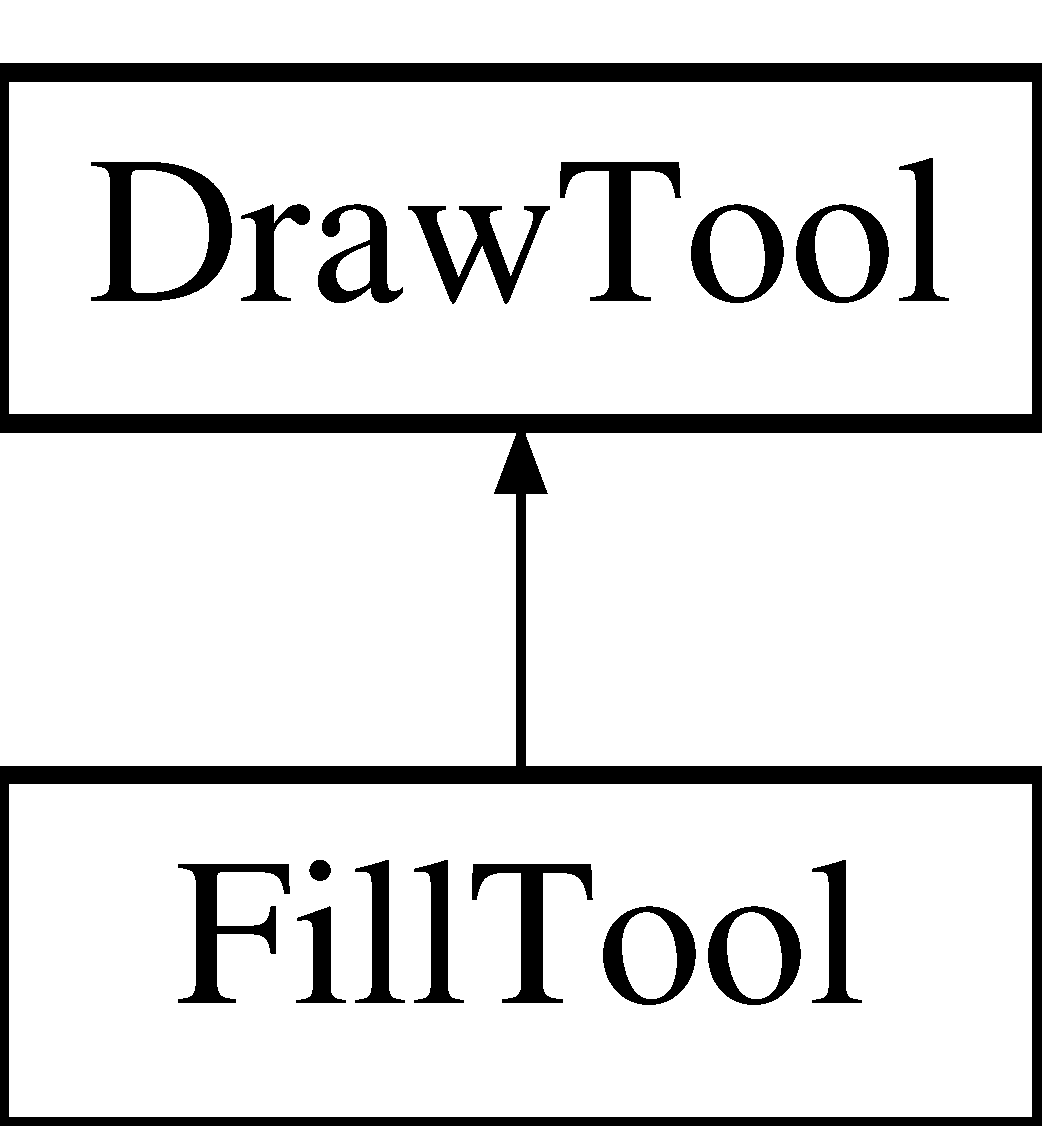
\includegraphics[height=2.000000cm]{classFillTool}
\end{center}
\end{figure}
\subsection*{Public Member Functions}
\begin{DoxyCompactItemize}
\item 
\hypertarget{classFillTool_a6abe3f5032f5e69a11cf38b94da90a62}{{\bfseries Fill\-Tool} (\hyperlink{classColorData}{Color\-Data} $\ast$tool\-Color, int height, int width)}\label{classFillTool_a6abe3f5032f5e69a11cf38b94da90a62}

\item 
\hypertarget{classFillTool_a81a3a46e5600d6250634766e8b769796}{void {\bfseries paint} (int x, int y, int prev\-X, int prev\-Y, \hyperlink{classPixelBuffer}{Pixel\-Buffer} $\ast$buffer)}\label{classFillTool_a81a3a46e5600d6250634766e8b769796}

\item 
\hypertarget{classFillTool_a8ad4d0d5b2a5379be3720c89a102ddb3}{void {\bfseries apply\-Influence} (int x, int y, \hyperlink{classPixelBuffer}{Pixel\-Buffer} $\ast$buffer)}\label{classFillTool_a8ad4d0d5b2a5379be3720c89a102ddb3}

\item 
\hypertarget{classFillTool_a888fd877cf0937e9b36be2d56f06de3e}{void {\bfseries fill\-Influence} ()}\label{classFillTool_a888fd877cf0937e9b36be2d56f06de3e}

\item 
\hypertarget{classFillTool_a6abe3f5032f5e69a11cf38b94da90a62}{{\bfseries Fill\-Tool} (\hyperlink{classColorData}{Color\-Data} $\ast$tool\-Color, int height, int width)}\label{classFillTool_a6abe3f5032f5e69a11cf38b94da90a62}

\item 
\hypertarget{classFillTool_a81a3a46e5600d6250634766e8b769796}{void {\bfseries paint} (int x, int y, int prev\-X, int prev\-Y, \hyperlink{classPixelBuffer}{Pixel\-Buffer} $\ast$buffer)}\label{classFillTool_a81a3a46e5600d6250634766e8b769796}

\item 
\hypertarget{classFillTool_a8ad4d0d5b2a5379be3720c89a102ddb3}{void {\bfseries apply\-Influence} (int x, int y, \hyperlink{classPixelBuffer}{Pixel\-Buffer} $\ast$buffer)}\label{classFillTool_a8ad4d0d5b2a5379be3720c89a102ddb3}

\item 
\hypertarget{classFillTool_a888fd877cf0937e9b36be2d56f06de3e}{void {\bfseries fill\-Influence} ()}\label{classFillTool_a888fd877cf0937e9b36be2d56f06de3e}

\item 
\hypertarget{classFillTool_a6abe3f5032f5e69a11cf38b94da90a62}{{\bfseries Fill\-Tool} (\hyperlink{classColorData}{Color\-Data} $\ast$tool\-Color, int height, int width)}\label{classFillTool_a6abe3f5032f5e69a11cf38b94da90a62}

\item 
\hypertarget{classFillTool_a81a3a46e5600d6250634766e8b769796}{void {\bfseries paint} (int x, int y, int prev\-X, int prev\-Y, \hyperlink{classPixelBuffer}{Pixel\-Buffer} $\ast$buffer)}\label{classFillTool_a81a3a46e5600d6250634766e8b769796}

\item 
\hypertarget{classFillTool_a8ad4d0d5b2a5379be3720c89a102ddb3}{void {\bfseries apply\-Influence} (int x, int y, \hyperlink{classPixelBuffer}{Pixel\-Buffer} $\ast$buffer)}\label{classFillTool_a8ad4d0d5b2a5379be3720c89a102ddb3}

\item 
\hypertarget{classFillTool_a888fd877cf0937e9b36be2d56f06de3e}{void {\bfseries fill\-Influence} ()}\label{classFillTool_a888fd877cf0937e9b36be2d56f06de3e}

\end{DoxyCompactItemize}
\subsection*{Additional Inherited Members}


The documentation for this class was generated from the following files\-:\begin{DoxyCompactItemize}
\item 
libphoto/Fill\-Tool.\-h\item 
libphoto/include/libphoto.\-h\item 
libphoto/Fill\-Tool.\-cpp\end{DoxyCompactItemize}

\hypertarget{classFilter}{\section{Filter Class Reference}
\label{classFilter}\index{Filter@{Filter}}
}
Inheritance diagram for Filter\-:\begin{figure}[H]
\begin{center}
\leavevmode
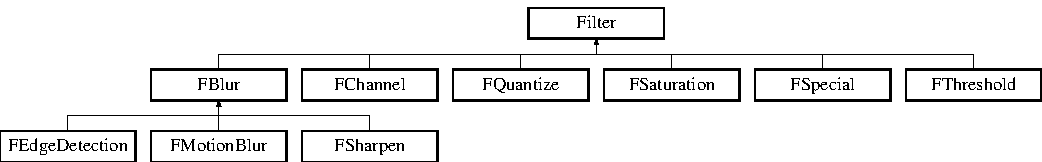
\includegraphics[height=2.181818cm]{classFilter}
\end{center}
\end{figure}
\subsection*{Public Member Functions}
\begin{DoxyCompactItemize}
\item 
\hypertarget{classFilter_a2ecb4bc0e81851d30f46f30bf81d1739}{virtual void {\bfseries apply\-Filter} (\hyperlink{classPixelBuffer}{Pixel\-Buffer} $\ast$image\-Buffer)=0}\label{classFilter_a2ecb4bc0e81851d30f46f30bf81d1739}

\item 
\hypertarget{classFilter_a212f40acb6481b2e36c3d129007519f1}{virtual std\-::string {\bfseries get\-Name} ()=0}\label{classFilter_a212f40acb6481b2e36c3d129007519f1}

\item 
\hypertarget{classFilter_aba015e9da647ba41fee4b41019d54516}{virtual void {\bfseries set\-Filter\-Parameter} (float parameter)}\label{classFilter_aba015e9da647ba41fee4b41019d54516}

\item 
\hypertarget{classFilter_a88314088e678c9a7cdbe0d0557385fa8}{virtual void {\bfseries set\-Filter\-Parameter} (\hyperlink{classColorData}{Color\-Data} parameter)}\label{classFilter_a88314088e678c9a7cdbe0d0557385fa8}

\item 
\hypertarget{classFilter_ada9d5f112e217c9bcf413093eae2a1e9}{void {\bfseries set\-Blur\-Direction} (int direction)}\label{classFilter_ada9d5f112e217c9bcf413093eae2a1e9}

\item 
\hypertarget{classFilter_a9f741b045bf1d57e485f116ce62ebac1}{float {\bfseries get\-Float\-Parameter} ()}\label{classFilter_a9f741b045bf1d57e485f116ce62ebac1}

\item 
\hypertarget{classFilter_abf85cdf0cda6dbe1dbcd6b8813aeecf3}{\hyperlink{classColorData}{Color\-Data} {\bfseries get\-Color\-Parameter} ()}\label{classFilter_abf85cdf0cda6dbe1dbcd6b8813aeecf3}

\item 
\hypertarget{classFilter_a465a168fc580c773e58d4df2f3db5968}{int {\bfseries get\-Blur\-Diection} ()}\label{classFilter_a465a168fc580c773e58d4df2f3db5968}

\end{DoxyCompactItemize}
\subsection*{Private Attributes}
\begin{DoxyCompactItemize}
\item 
\hypertarget{classFilter_a9bd610a1db8e1cde51f78b3a01b6638c}{float {\bfseries f\-\_\-parameter}}\label{classFilter_a9bd610a1db8e1cde51f78b3a01b6638c}

\item 
\hypertarget{classFilter_ab5464736d6dcb521cb14ac147f68ad7e}{\hyperlink{classColorData}{Color\-Data} {\bfseries c\-\_\-parameter}}\label{classFilter_ab5464736d6dcb521cb14ac147f68ad7e}

\item 
\hypertarget{classFilter_a05e0243ffe83143ba6c85084824be510}{int {\bfseries blur\-Direction}}\label{classFilter_a05e0243ffe83143ba6c85084824be510}

\end{DoxyCompactItemize}


The documentation for this class was generated from the following file\-:\begin{DoxyCompactItemize}
\item 
libphoto/Filter.\-h\end{DoxyCompactItemize}

\hypertarget{classFilterFactory}{\section{Filter\-Factory Class Reference}
\label{classFilterFactory}\index{Filter\-Factory@{Filter\-Factory}}
}
\subsection*{Public Types}
\begin{DoxyCompactItemize}
\item 
enum {\bfseries F\-I\-L\-T\-E\-R\-S} \{ \\*
{\bfseries F\-I\-L\-T\-E\-R\-\_\-\-T\-H\-R\-E\-S\-H\-O\-L\-D} = 0, 
{\bfseries F\-I\-L\-T\-E\-R\-\_\-\-C\-H\-A\-N\-N\-E\-L} = 1, 
{\bfseries F\-I\-L\-T\-E\-R\-\_\-\-S\-A\-T\-U\-R\-A\-T\-I\-O\-N} = 2, 
{\bfseries F\-I\-L\-T\-E\-R\-\_\-\-Q\-U\-A\-N\-T\-I\-Z\-E} = 3, 
\\*
{\bfseries F\-I\-L\-T\-E\-R\-\_\-\-B\-L\-U\-R} = 4, 
{\bfseries F\-I\-L\-T\-E\-R\-\_\-\-M\-O\-T\-I\-O\-N\-\_\-\-B\-L\-U\-R} = 5, 
{\bfseries F\-I\-L\-T\-E\-R\-\_\-\-S\-H\-A\-R\-P\-E\-N} = 6, 
{\bfseries F\-I\-L\-T\-E\-R\-\_\-\-D\-E\-T\-E\-C\-T\-\_\-\-E\-D\-G\-E\-S} = 7, 
\\*
{\bfseries F\-I\-L\-T\-E\-R\-\_\-\-S\-P\-E\-C\-I\-A\-L} = 8, 
{\bfseries N\-U\-M\-F\-I\-L\-T\-E\-R\-S} = 9
 \}
\end{DoxyCompactItemize}
\subsection*{Static Public Member Functions}
\begin{DoxyCompactItemize}
\item 
static int \hyperlink{classFilterFactory_a978466237a3acfbd5570fbf1d4dc1080}{get\-Num\-Filters} ()
\item 
static \hyperlink{classFilter}{Filter} $\ast$ \hyperlink{classFilterFactory_afa9986fc11ea262c26febc9191a19f47}{create\-Filter} (int filter\-I\-D)
\end{DoxyCompactItemize}


\subsection{Member Function Documentation}
\hypertarget{classFilterFactory_afa9986fc11ea262c26febc9191a19f47}{\index{Filter\-Factory@{Filter\-Factory}!create\-Filter@{create\-Filter}}
\index{create\-Filter@{create\-Filter}!FilterFactory@{Filter\-Factory}}
\subsubsection[{create\-Filter}]{\setlength{\rightskip}{0pt plus 5cm}{\bf Filter} $\ast$ Filter\-Factory\-::create\-Filter (
\begin{DoxyParamCaption}
\item[{int}]{filter\-I\-D}
\end{DoxyParamCaption}
)\hspace{0.3cm}{\ttfamily [static]}}}\label{classFilterFactory_afa9986fc11ea262c26febc9191a19f47}
Creates a filter for the given I\-D \par
param filter\-I\-D which filter you want to created \par
 return a filter instance \par
\hypertarget{classFilterFactory_a978466237a3acfbd5570fbf1d4dc1080}{\index{Filter\-Factory@{Filter\-Factory}!get\-Num\-Filters@{get\-Num\-Filters}}
\index{get\-Num\-Filters@{get\-Num\-Filters}!FilterFactory@{Filter\-Factory}}
\subsubsection[{get\-Num\-Filters}]{\setlength{\rightskip}{0pt plus 5cm}int Filter\-Factory\-::get\-Num\-Filters (
\begin{DoxyParamCaption}
{}
\end{DoxyParamCaption}
)\hspace{0.3cm}{\ttfamily [static]}}}\label{classFilterFactory_a978466237a3acfbd5570fbf1d4dc1080}
This is the \hyperlink{classFilterFactory}{Filter\-Factory} class, it is used to control the selection logic for filters. 

The documentation for this class was generated from the following files\-:\begin{DoxyCompactItemize}
\item 
libphoto/Filter\-Factory.\-h\item 
libphoto/Filter\-Factory.\-cpp\end{DoxyCompactItemize}

\hypertarget{classFlashPhotoApp}{\section{Flash\-Photo\-App Class Reference}
\label{classFlashPhotoApp}\index{Flash\-Photo\-App@{Flash\-Photo\-App}}
}
Inheritance diagram for Flash\-Photo\-App\-:\begin{figure}[H]
\begin{center}
\leavevmode
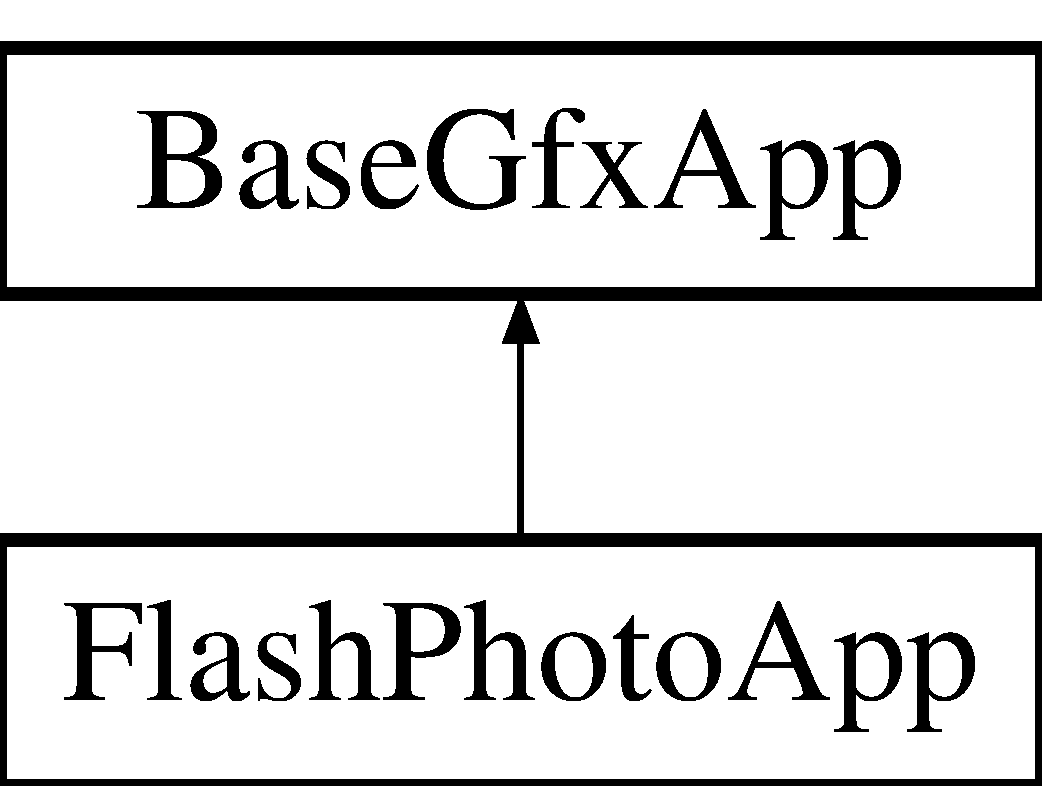
\includegraphics[height=2.000000cm]{classFlashPhotoApp}
\end{center}
\end{figure}
\subsection*{Public Member Functions}
\begin{DoxyCompactItemize}
\item 
\hyperlink{classFlashPhotoApp_a944931218613603cfb6bda6113971382}{Flash\-Photo\-App} (int argc, char $\ast$argv\mbox{[}$\,$\mbox{]}, int width, int height, \hyperlink{classColorData}{Color\-Data} background\-Color)
\item 
\hypertarget{classFlashPhotoApp_a29505b498fac898e099cfd1b8590c91a}{void \hyperlink{classFlashPhotoApp_a29505b498fac898e099cfd1b8590c91a}{mouse\-Dragged} (int x, int y)}\label{classFlashPhotoApp_a29505b498fac898e099cfd1b8590c91a}

\begin{DoxyCompactList}\small\item\em When the mouse is dragged this function is called. \end{DoxyCompactList}\item 
\hypertarget{classFlashPhotoApp_acf5a4cc5b76bb676d337758543bfdcc4}{void \hyperlink{classFlashPhotoApp_acf5a4cc5b76bb676d337758543bfdcc4}{mouse\-Moved} (int x, int y)}\label{classFlashPhotoApp_acf5a4cc5b76bb676d337758543bfdcc4}

\begin{DoxyCompactList}\small\item\em When the mouse if moved this function is called. \end{DoxyCompactList}\item 
\hypertarget{classFlashPhotoApp_a2c348ddcc15b6a21972bc6aac98c5442}{void \hyperlink{classFlashPhotoApp_a2c348ddcc15b6a21972bc6aac98c5442}{left\-Mouse\-Down} (int x, int y)}\label{classFlashPhotoApp_a2c348ddcc15b6a21972bc6aac98c5442}

\begin{DoxyCompactList}\small\item\em When the left mouse button is pressed this function is called. \end{DoxyCompactList}\item 
\hypertarget{classFlashPhotoApp_ae3a2f37b7c3657dcb5c16402c6d25519}{void \hyperlink{classFlashPhotoApp_ae3a2f37b7c3657dcb5c16402c6d25519}{left\-Mouse\-Up} (int x, int y)}\label{classFlashPhotoApp_ae3a2f37b7c3657dcb5c16402c6d25519}

\begin{DoxyCompactList}\small\item\em When the left mouse button is let go this function is called. \end{DoxyCompactList}\item 
\hypertarget{classFlashPhotoApp_a5dedc84bbc9ea0cf0718b8d0d0f414a5}{void {\bfseries display} ()}\label{classFlashPhotoApp_a5dedc84bbc9ea0cf0718b8d0d0f414a5}

\item 
\hypertarget{classFlashPhotoApp_aaeea3b8490d0f0239e41b781f6a066aa}{void {\bfseries glui\-Control} (int control\-I\-D)}\label{classFlashPhotoApp_aaeea3b8490d0f0239e41b781f6a066aa}

\end{DoxyCompactItemize}
\subsection*{Private Types}
\begin{DoxyCompactItemize}
\item 
enum {\bfseries U\-I\-Control\-Type} \{ \\*
{\bfseries U\-I\-\_\-\-T\-O\-O\-L\-T\-Y\-P\-E}, 
{\bfseries U\-I\-\_\-\-C\-O\-L\-O\-R\-\_\-\-R}, 
{\bfseries U\-I\-\_\-\-C\-O\-L\-O\-R\-\_\-\-G}, 
{\bfseries U\-I\-\_\-\-C\-O\-L\-O\-R\-\_\-\-B}, 
\\*
{\bfseries U\-I\-\_\-\-P\-R\-E\-S\-E\-T\-\_\-\-R\-E\-D}, 
{\bfseries U\-I\-\_\-\-P\-R\-E\-S\-E\-T\-\_\-\-O\-R\-A\-N\-G\-E}, 
{\bfseries U\-I\-\_\-\-P\-R\-E\-S\-E\-T\-\_\-\-Y\-E\-L\-L\-O\-W}, 
{\bfseries U\-I\-\_\-\-P\-R\-E\-S\-E\-T\-\_\-\-G\-R\-E\-E\-N}, 
\\*
{\bfseries U\-I\-\_\-\-P\-R\-E\-S\-E\-T\-\_\-\-B\-L\-U\-E}, 
{\bfseries U\-I\-\_\-\-P\-R\-E\-S\-E\-T\-\_\-\-P\-U\-R\-P\-L\-E}, 
{\bfseries U\-I\-\_\-\-P\-R\-E\-S\-E\-T\-\_\-\-W\-H\-I\-T\-E}, 
{\bfseries U\-I\-\_\-\-P\-R\-E\-S\-E\-T\-\_\-\-B\-L\-A\-C\-K}, 
\\*
{\bfseries U\-I\-\_\-\-F\-I\-L\-E\-\_\-\-B\-R\-O\-W\-S\-E\-R}, 
{\bfseries U\-I\-\_\-\-L\-O\-A\-D\-\_\-\-C\-A\-N\-V\-A\-S\-\_\-\-B\-U\-T\-T\-O\-N}, 
{\bfseries U\-I\-\_\-\-L\-O\-A\-D\-\_\-\-S\-T\-A\-M\-P\-\_\-\-B\-U\-T\-T\-O\-N}, 
{\bfseries U\-I\-\_\-\-S\-A\-V\-E\-\_\-\-C\-A\-N\-V\-A\-S\-\_\-\-B\-U\-T\-T\-O\-N}, 
\\*
{\bfseries U\-I\-\_\-\-F\-I\-L\-E\-\_\-\-N\-A\-M\-E}, 
{\bfseries U\-I\-\_\-\-A\-P\-P\-L\-Y\-\_\-\-B\-L\-U\-R}, 
{\bfseries U\-I\-\_\-\-A\-P\-P\-L\-Y\-\_\-\-S\-H\-A\-R\-P}, 
{\bfseries U\-I\-\_\-\-A\-P\-P\-L\-Y\-\_\-\-E\-D\-G\-E}, 
\\*
{\bfseries U\-I\-\_\-\-A\-P\-P\-L\-Y\-\_\-\-T\-H\-R\-E\-S\-H\-O\-L\-D}, 
{\bfseries U\-I\-\_\-\-A\-P\-P\-L\-Y\-\_\-\-D\-I\-T\-H\-E\-R}, 
{\bfseries U\-I\-\_\-\-A\-P\-P\-L\-Y\-\_\-\-S\-A\-T\-U\-R\-A\-T\-E}, 
{\bfseries U\-I\-\_\-\-A\-P\-P\-L\-Y\-\_\-\-C\-H\-A\-N\-N\-E\-L}, 
\\*
{\bfseries U\-I\-\_\-\-A\-P\-P\-L\-Y\-\_\-\-Q\-U\-A\-N\-T\-I\-Z\-E}, 
{\bfseries U\-I\-\_\-\-A\-P\-P\-L\-Y\-\_\-\-M\-O\-T\-I\-O\-N\-\_\-\-B\-L\-U\-R}, 
{\bfseries U\-I\-\_\-\-A\-P\-P\-L\-Y\-\_\-\-S\-P\-E\-C\-I\-A\-L\-\_\-\-F\-I\-L\-T\-E\-R}, 
{\bfseries U\-I\-\_\-\-U\-N\-D\-O}, 
\\*
{\bfseries U\-I\-\_\-\-R\-E\-D\-O}, 
{\bfseries U\-I\-\_\-\-C\-L\-E\-A\-R}, 
{\bfseries U\-I\-\_\-\-Q\-U\-I\-T}
 \}
\item 
enum {\bfseries U\-I\-Motion\-Blur\-Directions} \{ {\bfseries D\-I\-R\-\_\-\-N\-\_\-\-S}, 
{\bfseries D\-I\-R\-\_\-\-E\-\_\-\-W}, 
{\bfseries D\-I\-R\-\_\-\-N\-E\-\_\-\-S\-W}, 
{\bfseries D\-I\-R\-\_\-\-N\-W\-\_\-\-S\-E}
 \}
\item 
enum {\bfseries Tool\-Type} \{ \\*
{\bfseries P\-E\-N}, 
{\bfseries E\-R\-A\-S\-E\-R}, 
{\bfseries S\-P\-R\-A\-Y\-C\-A\-N}, 
{\bfseries C\-A\-L\-I\-G\-R\-A\-P\-H\-Y\-P\-E\-N}, 
\\*
{\bfseries H\-I\-G\-H\-L\-I\-G\-H\-T\-E\-R}, 
{\bfseries W\-A\-T\-E\-R\-C\-O\-L\-O\-R}, 
{\bfseries F\-I\-L\-L\-T\-O\-O\-L}, 
{\bfseries C\-R\-A\-Y\-O\-N}, 
\\*
{\bfseries S\-T\-A\-M\-P}, 
{\bfseries B\-L\-U\-R}
 \}
\end{DoxyCompactItemize}
\subsection*{Private Member Functions}
\begin{DoxyCompactItemize}
\item 
\hypertarget{classFlashPhotoApp_a262d3fad41e5feb441b4ea431c65f8c1}{void {\bfseries set\-Image\-File} (const std\-::string \&filepath)}\label{classFlashPhotoApp_a262d3fad41e5feb441b4ea431c65f8c1}

\item 
\hypertarget{classFlashPhotoApp_a05fb136c74949eb11f07f161e18b0e44}{bool {\bfseries is\-Valid\-Image\-File\-Name} (const std\-::string \&name)}\label{classFlashPhotoApp_a05fb136c74949eb11f07f161e18b0e44}

\item 
\hypertarget{classFlashPhotoApp_af9f413e89445c3a0210e69d542affd67}{bool {\bfseries is\-Valid\-Image\-File} (const std\-::string \&name)}\label{classFlashPhotoApp_af9f413e89445c3a0210e69d542affd67}

\item 
\hypertarget{classFlashPhotoApp_a346a7760598d8dd3c6ddb0630b1e51b6}{bool {\bfseries has\-Suffix} (const std\-::string \&str, const std\-::string \&suffix)}\label{classFlashPhotoApp_a346a7760598d8dd3c6ddb0630b1e51b6}

\item 
\hypertarget{classFlashPhotoApp_a886a76eaa5e30c1708a96cc62cd98887}{void {\bfseries button\-Enabled} (G\-L\-U\-I\-\_\-\-Button $\ast$button, bool enabled)}\label{classFlashPhotoApp_a886a76eaa5e30c1708a96cc62cd98887}

\item 
\hypertarget{classFlashPhotoApp_aa4ceaa973c4cd8b953e4e09d0a5a81ff}{void {\bfseries undo\-Enabled} (bool enabled)}\label{classFlashPhotoApp_aa4ceaa973c4cd8b953e4e09d0a5a81ff}

\item 
\hypertarget{classFlashPhotoApp_a03e224580f502076a6c498a35fb8069f}{void {\bfseries redo\-Enabled} (bool enabled)}\label{classFlashPhotoApp_a03e224580f502076a6c498a35fb8069f}

\item 
\hypertarget{classFlashPhotoApp_af370462c4a82dd932ae7364fc58e3959}{void {\bfseries save\-Canvas\-Enabled} (bool enabled)}\label{classFlashPhotoApp_af370462c4a82dd932ae7364fc58e3959}

\item 
\hypertarget{classFlashPhotoApp_aa04f2738fdb07a7eaa86f146c7537a70}{void {\bfseries load\-Canvas\-Enabled} (bool enabled)}\label{classFlashPhotoApp_aa04f2738fdb07a7eaa86f146c7537a70}

\item 
\hypertarget{classFlashPhotoApp_a9e58a2c36d94fcbe376f3cb5b75ad5e0}{void {\bfseries load\-Stamp\-Enabled} (bool enabled)}\label{classFlashPhotoApp_a9e58a2c36d94fcbe376f3cb5b75ad5e0}

\item 
\hypertarget{classFlashPhotoApp_ad554624b8359abe270e5c6e76634ff48}{void {\bfseries update\-Colors} ()}\label{classFlashPhotoApp_ad554624b8359abe270e5c6e76634ff48}

\item 
void \hyperlink{classFlashPhotoApp_a29383606562f09ba623209581f92f5e5}{init\-Draw\-Tool} ()
\item 
void \hyperlink{classFlashPhotoApp_aeaf85d6ead6ca4b3905701db12ceaf68}{init\-Filter} ()
\item 
void \hyperlink{classFlashPhotoApp_a52eb2524a928df150d75492d96a3d49c}{update\-Current\-Tool} ()
\item 
void \hyperlink{classFlashPhotoApp_a7cc9f1383c18cb7eebc255d3c377adb0}{load\-Image\-To\-Canvas} ()
\item 
\hypertarget{classFlashPhotoApp_a87aee2ef5baef954b682c67e3d5118da}{void {\bfseries load\-Image\-To\-Stamp} ()}\label{classFlashPhotoApp_a87aee2ef5baef954b682c67e3d5118da}

\item 
void \hyperlink{classFlashPhotoApp_ab0389fb3c2c64e0e3312880e745b7070}{save\-Canvas\-To\-File} ()
\item 
\hypertarget{classFlashPhotoApp_a16ff3baa9c0d97d8e4f292acb4ebbfac}{void {\bfseries apply\-Filter\-Blur} ()}\label{classFlashPhotoApp_a16ff3baa9c0d97d8e4f292acb4ebbfac}

\item 
\hypertarget{classFlashPhotoApp_a9d45a9f24245024cba2c9090d7acb528}{void {\bfseries apply\-Filter\-Sharpen} ()}\label{classFlashPhotoApp_a9d45a9f24245024cba2c9090d7acb528}

\item 
\hypertarget{classFlashPhotoApp_af99c135d287d07e01ccd1637cba0d347}{void {\bfseries apply\-Filter\-Motion\-Blur} ()}\label{classFlashPhotoApp_af99c135d287d07e01ccd1637cba0d347}

\item 
\hypertarget{classFlashPhotoApp_ae7360d5fc26c2789d0126defb1c30e9f}{void {\bfseries apply\-Filter\-Edge\-Detect} ()}\label{classFlashPhotoApp_ae7360d5fc26c2789d0126defb1c30e9f}

\item 
\hypertarget{classFlashPhotoApp_a316479ee5fc48b785c266953147de63e}{void {\bfseries apply\-Filter\-Threshold} ()}\label{classFlashPhotoApp_a316479ee5fc48b785c266953147de63e}

\item 
\hypertarget{classFlashPhotoApp_a8c8d8c714d059083f49e1e0cd1336321}{void {\bfseries apply\-Filter\-Channel} ()}\label{classFlashPhotoApp_a8c8d8c714d059083f49e1e0cd1336321}

\item 
\hypertarget{classFlashPhotoApp_aabd2e2b487ebe038cbcbfa700d5951f9}{void {\bfseries apply\-Filter\-Saturate} ()}\label{classFlashPhotoApp_aabd2e2b487ebe038cbcbfa700d5951f9}

\item 
\hypertarget{classFlashPhotoApp_a5a9c62db1aa83250b4f95c94f5dac762}{void {\bfseries apply\-Filter\-Quantize} ()}\label{classFlashPhotoApp_a5a9c62db1aa83250b4f95c94f5dac762}

\item 
\hypertarget{classFlashPhotoApp_a7b1664e842e4a0a16cf7c340e126de17}{void {\bfseries apply\-Filter\-Special} ()}\label{classFlashPhotoApp_a7b1664e842e4a0a16cf7c340e126de17}

\item 
\hypertarget{classFlashPhotoApp_ad33153aceb1cca61bb682c00ae8e22ff}{void {\bfseries undo\-Operation} ()}\label{classFlashPhotoApp_ad33153aceb1cca61bb682c00ae8e22ff}

\item 
\hypertarget{classFlashPhotoApp_aad1a00932e723e17c39f6959c42d9f5f}{void {\bfseries redo\-Operation} ()}\label{classFlashPhotoApp_aad1a00932e723e17c39f6959c42d9f5f}

\item 
void \hyperlink{classFlashPhotoApp_af90d307fdc027a037816a63757a17120}{update\-Canvas} (std\-::deque$<$ \hyperlink{classPixelBuffer}{Pixel\-Buffer} $\ast$ $>$ \&alpha, std\-::deque$<$ \hyperlink{classPixelBuffer}{Pixel\-Buffer} $\ast$ $>$ \&beta, bool is\-Undo)
\item 
\hypertarget{classFlashPhotoApp_a8360b752328c423d850d819361e18a12}{void {\bfseries init\-Glui} ()}\label{classFlashPhotoApp_a8360b752328c423d850d819361e18a12}

\item 
\hypertarget{classFlashPhotoApp_a9a786ee86c70c142fd957421f9354996}{void {\bfseries init\-Graphics} ()}\label{classFlashPhotoApp_a9a786ee86c70c142fd957421f9354996}

\item 
\hypertarget{classFlashPhotoApp_afed06134c0c49494fb5055a93dc8423f}{void {\bfseries initialize\-Buffers} (\hyperlink{classColorData}{Color\-Data} initial\-Color, int width, int height)}\label{classFlashPhotoApp_afed06134c0c49494fb5055a93dc8423f}

\item 
\hypertarget{classFlashPhotoApp_a2dc3dd9da509fb67ab5ae61b6a8d9c03}{bool {\bfseries isjpeg} (const std\-::string \&name)}\label{classFlashPhotoApp_a2dc3dd9da509fb67ab5ae61b6a8d9c03}

\item 
\hypertarget{classFlashPhotoApp_aa53b230edec12feb0ed4e5531cdd760e}{int {\bfseries loadpng} (F\-I\-L\-E $\ast$fp)}\label{classFlashPhotoApp_aa53b230edec12feb0ed4e5531cdd760e}

\item 
void \hyperlink{classFlashPhotoApp_a7dc31c434067d59fa14d40e22a21d66c}{clear\-Pixel\-Buffer} ()
\item 
\hypertarget{classFlashPhotoApp_ae578c10b12f1f39d52d2fe2e4f0f5b96}{void {\bfseries update\-Undo} ()}\label{classFlashPhotoApp_ae578c10b12f1f39d52d2fe2e4f0f5b96}

\end{DoxyCompactItemize}
\subsection*{Private Attributes}
\begin{DoxyCompactItemize}
\item 
\hypertarget{classFlashPhotoApp_adc1082b61b8e0650f8dba72e0ac9c90d}{\begin{tabbing}
xx\=xx\=xx\=xx\=xx\=xx\=xx\=xx\=xx\=\kill
struct \{\\
\hypertarget{structFlashPhotoApp_1_1@0_a24bac49f0d04130b0012f82c7683afac}{\>float {\bfseries channel\_colorRed}\\
\hypertarget{structFlashPhotoApp_1_1@0_ac18742e7fcb8534d9476c100d742358d}{\>float {\bfseries channel\_colorGreen}\\
\hypertarget{structFlashPhotoApp_1_1@0_aaad046817775345700256c63ee69a066}{\>float {\bfseries channel\_colorBlue}\\
\hypertarget{structFlashPhotoApp_1_1@0_a507851bce4f4af02c093a1d28a088da7}{\>float {\bfseries saturation\_amount}\\
\hypertarget{structFlashPhotoApp_1_1@0_a47e02008d3de690cd60c97df03e4d8fd}{\>float {\bfseries threshold\_amount}\\
\hypertarget{structFlashPhotoApp_1_1@0_abe620dc3be32a15e2a87426eae4b9429}{\>float {\bfseries blur\_amount}\\
\hypertarget{structFlashPhotoApp_1_1@0_ab8ddc9587fc24a36c5eb1ddf1380ef99}{\>float {\bfseries sharpen\_amount}\\
\hypertarget{structFlashPhotoApp_1_1@0_a224bd3b1ac652128da1736dbd855a467}{\>float {\bfseries motionBlur\_amount}\\
\hypertarget{structFlashPhotoApp_1_1@0_a37732ed053efaac3198792777abc537a}{\>int {\bfseries motionBlur\_direction}\\
\hypertarget{structFlashPhotoApp_1_1@0_a21466a62d5a49b29052541c1bdaaff82}{\>int {\bfseries quantize\_bins}\\
\} {\bfseries m\_filterParameters}}\label{classFlashPhotoApp_adc1082b61b8e0650f8dba72e0ac9c90d}
\\

\end{tabbing}\item 
\hypertarget{classFlashPhotoApp_a26ed03c8eea24f9b2193fe98f02a78b7}{\begin{tabbing}
xx\=xx\=xx\=xx\=xx\=xx\=xx\=xx\=xx\=\kill
struct \{\\
\hypertarget{structFlashPhotoApp_1_1@1_a6e190905f22d88f7155b5e4fea7e82e2}{\>GLUI\_FileBrowser $\ast$ {\bfseries fileBrowser}\\
\hypertarget{structFlashPhotoApp_1_1@1_a568203b21cda88b7f64a5339064a7d18}{\>GLUI\_Button $\ast$ {\bfseries loadCanvasButton}\\
\hypertarget{structFlashPhotoApp_1_1@1_aa4aa83844dfbaac5e2601d9ecf252e60}{\>GLUI\_Button $\ast$ {\bfseries loadStampButton}\\
\hypertarget{structFlashPhotoApp_1_1@1_a1b1c7930ccf25d66161aa0bd0926f885}{\>GLUI\_Button $\ast$ {\bfseries saveCanvasButton}\\
\hypertarget{structFlashPhotoApp_1_1@1_a96d62cf788203344f8941b79170fc346}{\>GLUI\_Button $\ast$ {\bfseries redoButton}\\
\hypertarget{structFlashPhotoApp_1_1@1_abce09e914786f07c8de6e675574e7681}{\>GLUI\_Button $\ast$ {\bfseries undoButton}\\
\hypertarget{structFlashPhotoApp_1_1@1_af6bf7b007ec57149ac322bb039b36448}{\>GLUI\_StaticText $\ast$ {\bfseries currentFileLabel}\\
\hypertarget{structFlashPhotoApp_1_1@1_abe3d1fbda64a09063e4d3a5f33c1d860}{\>GLUI\_EditText $\ast$ {\bfseries fileNameBox}\\
\hypertarget{structFlashPhotoApp_1_1@1_a830a100998dba74fbb5c71566ae20460}{\>GLUI\_StaticText $\ast$ {\bfseries saveFileLabel}\\
\hypertarget{structFlashPhotoApp_1_1@1_a54d8c8487ee6d847b9dc38f3f03f78db}{\>GLUI\_Spinner $\ast$ {\bfseries spinnerRed}\\
\hypertarget{structFlashPhotoApp_1_1@1_ac912473a2801aa9bfe9fcf1072e48627}{\>GLUI\_Spinner $\ast$ {\bfseries spinnerGreen}\\
\hypertarget{structFlashPhotoApp_1_1@1_acc6dc220ee767f7b5b113e26ddbc18b9}{\>GLUI\_Spinner $\ast$ {\bfseries spinnerBlue}\\
\} {\bfseries m\_gluiControlHooks}}\label{classFlashPhotoApp_a26ed03c8eea24f9b2193fe98f02a78b7}
\\

\end{tabbing}\item 
\hypertarget{classFlashPhotoApp_ae45bc3761686cbb4d5f9c01b048816c0}{int {\bfseries m\-\_\-queue\-Size}}\label{classFlashPhotoApp_ae45bc3761686cbb4d5f9c01b048816c0}

\item 
\hypertarget{classFlashPhotoApp_abdb0f4d46432039c14d5816abb019fa7}{std\-::deque$<$ \hyperlink{classPixelBuffer}{Pixel\-Buffer} $\ast$ $>$ {\bfseries undo\-Queue}}\label{classFlashPhotoApp_abdb0f4d46432039c14d5816abb019fa7}

\item 
\hypertarget{classFlashPhotoApp_a67142e2e575f5c63666b3e750279fd4f}{std\-::deque$<$ \hyperlink{classPixelBuffer}{Pixel\-Buffer} $\ast$ $>$ {\bfseries redo\-Queue}}\label{classFlashPhotoApp_a67142e2e575f5c63666b3e750279fd4f}

\item 
\hypertarget{classFlashPhotoApp_a7552f6cf6441c53d020e5a0124031bcb}{int {\bfseries m\-\_\-prev\-X}}\label{classFlashPhotoApp_a7552f6cf6441c53d020e5a0124031bcb}

\item 
\hypertarget{classFlashPhotoApp_a6a9759bdfbdf16bf0091f1694604a64a}{int {\bfseries m\-\_\-prev\-Y}}\label{classFlashPhotoApp_a6a9759bdfbdf16bf0091f1694604a64a}

\item 
\hypertarget{classFlashPhotoApp_a2e397b37bfb3ea981efc795b7a2a9e9e}{int {\bfseries m\-\_\-stamp\-Height}}\label{classFlashPhotoApp_a2e397b37bfb3ea981efc795b7a2a9e9e}

\item 
\hypertarget{classFlashPhotoApp_a7dab8bf3eb60e4c99310660c9c32f3a5}{int {\bfseries m\-\_\-stamp\-Width}}\label{classFlashPhotoApp_a7dab8bf3eb60e4c99310660c9c32f3a5}

\item 
\hypertarget{classFlashPhotoApp_a9662e1dbd6e003a62179eecba827e910}{\hyperlink{classPixelBuffer}{Pixel\-Buffer} $\ast$ {\bfseries m\-\_\-display\-Buffer}}\label{classFlashPhotoApp_a9662e1dbd6e003a62179eecba827e910}

\item 
\hypertarget{classFlashPhotoApp_a752ba29ca132a3fd4deaa3727946f7f6}{\hyperlink{classDrawTool}{Draw\-Tool} $\ast$$\ast$ {\bfseries tool\-List}}\label{classFlashPhotoApp_a752ba29ca132a3fd4deaa3727946f7f6}

\item 
\hypertarget{classFlashPhotoApp_a69d8dcf7147882964a6d2832bbab67e2}{\hyperlink{classDrawTool}{Draw\-Tool} $\ast$ {\bfseries m\-\_\-tool}}\label{classFlashPhotoApp_a69d8dcf7147882964a6d2832bbab67e2}

\item 
\hypertarget{classFlashPhotoApp_a4fe8a885ae7b5e698c40a7585b4e292d}{int {\bfseries m\-\_\-cur\-Tool}}\label{classFlashPhotoApp_a4fe8a885ae7b5e698c40a7585b4e292d}

\item 
\hypertarget{classFlashPhotoApp_a40ef9e2d21c3f80cee59be363e21b9bc}{\hyperlink{classFilter}{Filter} $\ast$$\ast$ {\bfseries m\-\_\-filters}}\label{classFlashPhotoApp_a40ef9e2d21c3f80cee59be363e21b9bc}

\item 
\hypertarget{classFlashPhotoApp_a584dd16d8f2aad51028759a1dd94c83f}{int {\bfseries m\-\_\-cur\-Filter}}\label{classFlashPhotoApp_a584dd16d8f2aad51028759a1dd94c83f}

\item 
\hypertarget{classFlashPhotoApp_a6e4b0ca13b038233f14563c79f7201ae}{float {\bfseries m\-\_\-cur\-Color\-Red}}\label{classFlashPhotoApp_a6e4b0ca13b038233f14563c79f7201ae}

\item 
\hypertarget{classFlashPhotoApp_a3af18066365495dda69e11a3b5116ee6}{float {\bfseries m\-\_\-cur\-Color\-Green}}\label{classFlashPhotoApp_a3af18066365495dda69e11a3b5116ee6}

\item 
\hypertarget{classFlashPhotoApp_a1c7b40fbfe40343ff9653120b6925f09}{float {\bfseries m\-\_\-cur\-Color\-Blue}}\label{classFlashPhotoApp_a1c7b40fbfe40343ff9653120b6925f09}

\item 
\hypertarget{classFlashPhotoApp_a110a669df9d98f66a68b9d2eec6a9748}{std\-::string {\bfseries m\-\_\-file\-Name}}\label{classFlashPhotoApp_a110a669df9d98f66a68b9d2eec6a9748}

\end{DoxyCompactItemize}
\subsection*{Additional Inherited Members}


\subsection{Constructor \& Destructor Documentation}
\hypertarget{classFlashPhotoApp_a944931218613603cfb6bda6113971382}{\index{Flash\-Photo\-App@{Flash\-Photo\-App}!Flash\-Photo\-App@{Flash\-Photo\-App}}
\index{Flash\-Photo\-App@{Flash\-Photo\-App}!FlashPhotoApp@{Flash\-Photo\-App}}
\subsubsection[{Flash\-Photo\-App}]{\setlength{\rightskip}{0pt plus 5cm}Flash\-Photo\-App\-::\-Flash\-Photo\-App (
\begin{DoxyParamCaption}
\item[{int}]{argc, }
\item[{char $\ast$}]{argv\mbox{[}$\,$\mbox{]}, }
\item[{int}]{width, }
\item[{int}]{height, }
\item[{{\bf Color\-Data}}]{background\-Color}
\end{DoxyParamCaption}
)}}\label{classFlashPhotoApp_a944931218613603cfb6bda6113971382}
This is the Flash\-Photo class. This class contains all of the main U\-I login for the application. 

\subsection{Member Function Documentation}
\hypertarget{classFlashPhotoApp_a7dc31c434067d59fa14d40e22a21d66c}{\index{Flash\-Photo\-App@{Flash\-Photo\-App}!clear\-Pixel\-Buffer@{clear\-Pixel\-Buffer}}
\index{clear\-Pixel\-Buffer@{clear\-Pixel\-Buffer}!FlashPhotoApp@{Flash\-Photo\-App}}
\subsubsection[{clear\-Pixel\-Buffer}]{\setlength{\rightskip}{0pt plus 5cm}void Flash\-Photo\-App\-::clear\-Pixel\-Buffer (
\begin{DoxyParamCaption}
{}
\end{DoxyParamCaption}
)\hspace{0.3cm}{\ttfamily [private]}}}\label{classFlashPhotoApp_a7dc31c434067d59fa14d40e22a21d66c}
Clear the pixel buffer back to the default buffer color \par
none \par
void \par
\hypertarget{classFlashPhotoApp_a29383606562f09ba623209581f92f5e5}{\index{Flash\-Photo\-App@{Flash\-Photo\-App}!init\-Draw\-Tool@{init\-Draw\-Tool}}
\index{init\-Draw\-Tool@{init\-Draw\-Tool}!FlashPhotoApp@{Flash\-Photo\-App}}
\subsubsection[{init\-Draw\-Tool}]{\setlength{\rightskip}{0pt plus 5cm}void Flash\-Photo\-App\-::init\-Draw\-Tool (
\begin{DoxyParamCaption}
{}
\end{DoxyParamCaption}
)\hspace{0.3cm}{\ttfamily [private]}}}\label{classFlashPhotoApp_a29383606562f09ba623209581f92f5e5}
Initialize the draw tool on load \par
none \par
void \par
\hypertarget{classFlashPhotoApp_aeaf85d6ead6ca4b3905701db12ceaf68}{\index{Flash\-Photo\-App@{Flash\-Photo\-App}!init\-Filter@{init\-Filter}}
\index{init\-Filter@{init\-Filter}!FlashPhotoApp@{Flash\-Photo\-App}}
\subsubsection[{init\-Filter}]{\setlength{\rightskip}{0pt plus 5cm}void Flash\-Photo\-App\-::init\-Filter (
\begin{DoxyParamCaption}
{}
\end{DoxyParamCaption}
)\hspace{0.3cm}{\ttfamily [private]}}}\label{classFlashPhotoApp_aeaf85d6ead6ca4b3905701db12ceaf68}
Initialize the filter on load \par
none \par
void \par
\hypertarget{classFlashPhotoApp_a7cc9f1383c18cb7eebc255d3c377adb0}{\index{Flash\-Photo\-App@{Flash\-Photo\-App}!load\-Image\-To\-Canvas@{load\-Image\-To\-Canvas}}
\index{load\-Image\-To\-Canvas@{load\-Image\-To\-Canvas}!FlashPhotoApp@{Flash\-Photo\-App}}
\subsubsection[{load\-Image\-To\-Canvas}]{\setlength{\rightskip}{0pt plus 5cm}void Flash\-Photo\-App\-::load\-Image\-To\-Canvas (
\begin{DoxyParamCaption}
{}
\end{DoxyParamCaption}
)\hspace{0.3cm}{\ttfamily [private]}}}\label{classFlashPhotoApp_a7cc9f1383c18cb7eebc255d3c377adb0}
Load an image on to the canvas \par
none \par
void \par
\hypertarget{classFlashPhotoApp_ab0389fb3c2c64e0e3312880e745b7070}{\index{Flash\-Photo\-App@{Flash\-Photo\-App}!save\-Canvas\-To\-File@{save\-Canvas\-To\-File}}
\index{save\-Canvas\-To\-File@{save\-Canvas\-To\-File}!FlashPhotoApp@{Flash\-Photo\-App}}
\subsubsection[{save\-Canvas\-To\-File}]{\setlength{\rightskip}{0pt plus 5cm}void Flash\-Photo\-App\-::save\-Canvas\-To\-File (
\begin{DoxyParamCaption}
{}
\end{DoxyParamCaption}
)\hspace{0.3cm}{\ttfamily [private]}}}\label{classFlashPhotoApp_ab0389fb3c2c64e0e3312880e745b7070}
Save a canvas to file \par
none \par
void \par
\hypertarget{classFlashPhotoApp_af90d307fdc027a037816a63757a17120}{\index{Flash\-Photo\-App@{Flash\-Photo\-App}!update\-Canvas@{update\-Canvas}}
\index{update\-Canvas@{update\-Canvas}!FlashPhotoApp@{Flash\-Photo\-App}}
\subsubsection[{update\-Canvas}]{\setlength{\rightskip}{0pt plus 5cm}void Flash\-Photo\-App\-::update\-Canvas (
\begin{DoxyParamCaption}
\item[{std\-::deque$<$ {\bf Pixel\-Buffer} $\ast$ $>$ \&}]{alpha, }
\item[{std\-::deque$<$ {\bf Pixel\-Buffer} $\ast$ $>$ \&}]{beta, }
\item[{bool}]{is\-Undo}
\end{DoxyParamCaption}
)\hspace{0.3cm}{\ttfamily [private]}}}\label{classFlashPhotoApp_af90d307fdc027a037816a63757a17120}
Update the canvas with the top of the alpha deque, push current buffer onto beta deque \par
deque to pop from, deque to push to, if it is an undo \par
void \par
\hypertarget{classFlashPhotoApp_a52eb2524a928df150d75492d96a3d49c}{\index{Flash\-Photo\-App@{Flash\-Photo\-App}!update\-Current\-Tool@{update\-Current\-Tool}}
\index{update\-Current\-Tool@{update\-Current\-Tool}!FlashPhotoApp@{Flash\-Photo\-App}}
\subsubsection[{update\-Current\-Tool}]{\setlength{\rightskip}{0pt plus 5cm}void Flash\-Photo\-App\-::update\-Current\-Tool (
\begin{DoxyParamCaption}
{}
\end{DoxyParamCaption}
)\hspace{0.3cm}{\ttfamily [private]}}}\label{classFlashPhotoApp_a52eb2524a928df150d75492d96a3d49c}
Update the current tool that is selected in the U\-I (stored in m\-\_\-cur\-Tool) \par
none \par
void \par


The documentation for this class was generated from the following files\-:\begin{DoxyCompactItemize}
\item 
Flash\-Photo/Flash\-Photo\-App.\-h\item 
Flash\-Photo/Flash\-Photo\-App.\-cpp\end{DoxyCompactItemize}

\hypertarget{classFMotionBlur}{\section{F\-Motion\-Blur Class Reference}
\label{classFMotionBlur}\index{F\-Motion\-Blur@{F\-Motion\-Blur}}
}
Inheritance diagram for F\-Motion\-Blur\-:\begin{figure}[H]
\begin{center}
\leavevmode
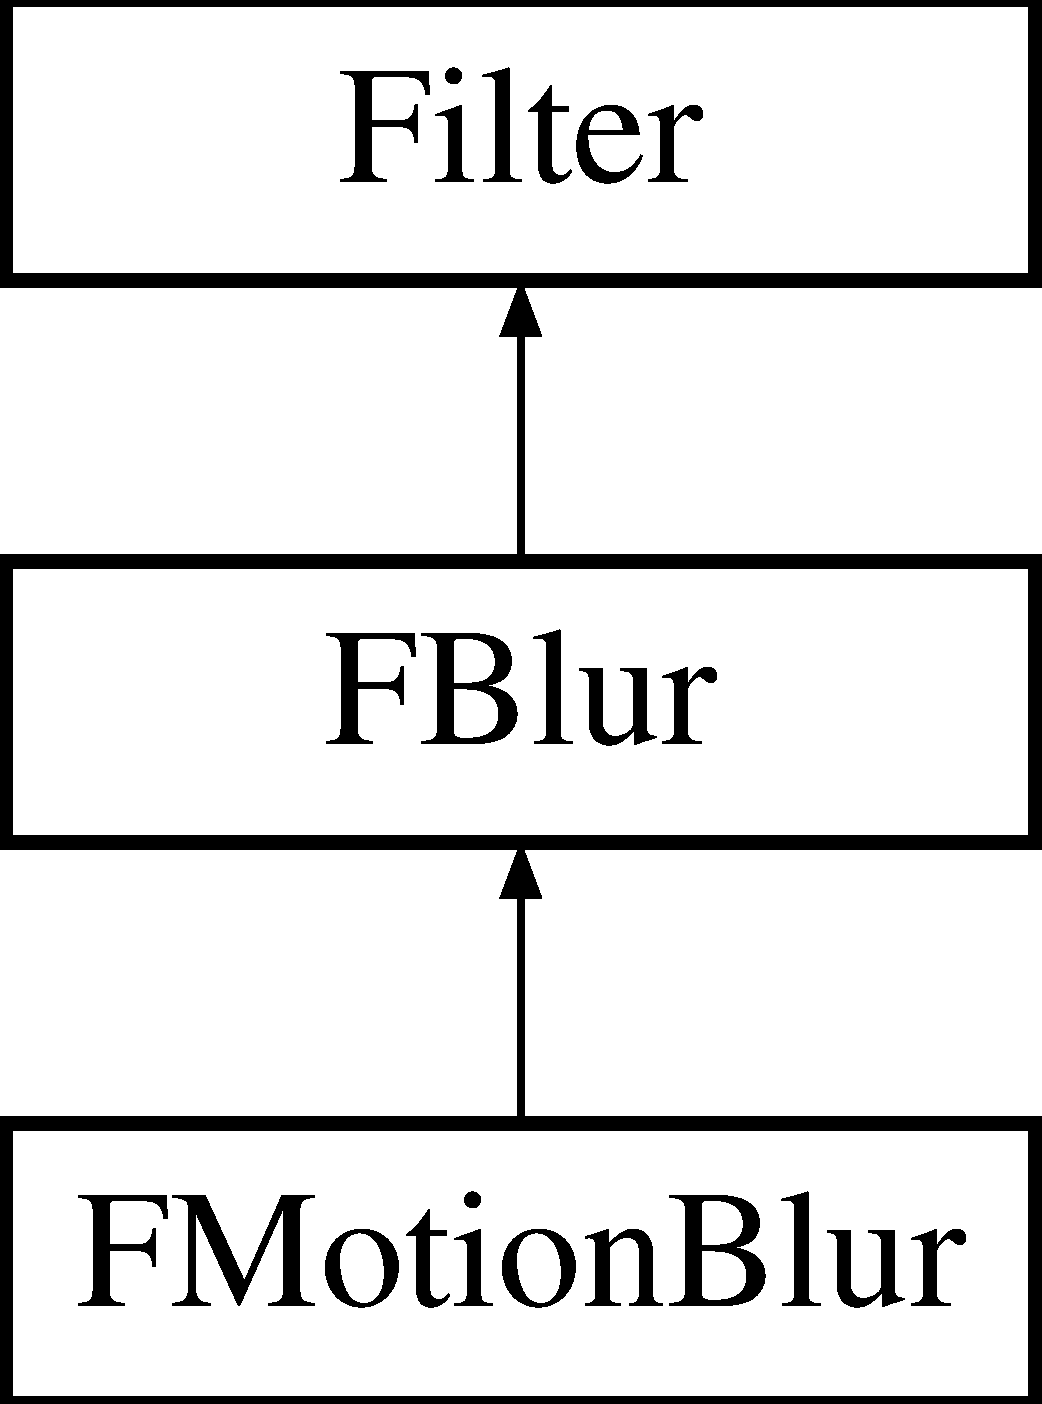
\includegraphics[height=3.000000cm]{classFMotionBlur}
\end{center}
\end{figure}
\subsection*{Public Types}
\begin{DoxyCompactItemize}
\item 
enum {\bfseries Motion\-Blur\-Directions} \{ {\bfseries D\-I\-R\-\_\-\-N\-\_\-\-S}, 
{\bfseries D\-I\-R\-\_\-\-E\-\_\-\-W}, 
{\bfseries D\-I\-R\-\_\-\-N\-E\-\_\-\-S\-W}, 
{\bfseries D\-I\-R\-\_\-\-N\-W\-\_\-\-S\-E}
 \}
\end{DoxyCompactItemize}
\subsection*{Public Member Functions}
\begin{DoxyCompactItemize}
\item 
\hyperlink{classFMotionBlur_a670df8e9b43ff1ff3b262b6d48b944cf}{F\-Motion\-Blur} ()
\item 
\hypertarget{classFMotionBlur_aeb40f52478dcf27d5fa8fec4aa473975}{std\-::string {\bfseries get\-Name} ()}\label{classFMotionBlur_aeb40f52478dcf27d5fa8fec4aa473975}

\item 
\hypertarget{classFMotionBlur_a105abc618c4fe5ddd890ad2ff1836979}{kernel\-Type {\bfseries build\-Kernel} (int radius)}\label{classFMotionBlur_a105abc618c4fe5ddd890ad2ff1836979}

\end{DoxyCompactItemize}


\subsection{Constructor \& Destructor Documentation}
\hypertarget{classFMotionBlur_a670df8e9b43ff1ff3b262b6d48b944cf}{\index{F\-Motion\-Blur@{F\-Motion\-Blur}!F\-Motion\-Blur@{F\-Motion\-Blur}}
\index{F\-Motion\-Blur@{F\-Motion\-Blur}!FMotionBlur@{F\-Motion\-Blur}}
\subsubsection[{F\-Motion\-Blur}]{\setlength{\rightskip}{0pt plus 5cm}F\-Motion\-Blur\-::\-F\-Motion\-Blur (
\begin{DoxyParamCaption}
{}
\end{DoxyParamCaption}
)}}\label{classFMotionBlur_a670df8e9b43ff1ff3b262b6d48b944cf}
This is the F\-Motion class, it is used for the motion blur image filters. It inherits from the \hyperlink{classFBlur}{F\-Blur} class, so it only needs to build\-Kernel, not apply it. 

The documentation for this class was generated from the following files\-:\begin{DoxyCompactItemize}
\item 
libphoto/F\-Motion\-Blur.\-h\item 
libphoto/F\-Motion\-Blur.\-cpp\end{DoxyCompactItemize}

\hypertarget{classFQuantize}{\section{F\-Quantize Class Reference}
\label{classFQuantize}\index{F\-Quantize@{F\-Quantize}}
}
Inheritance diagram for F\-Quantize\-:\begin{figure}[H]
\begin{center}
\leavevmode
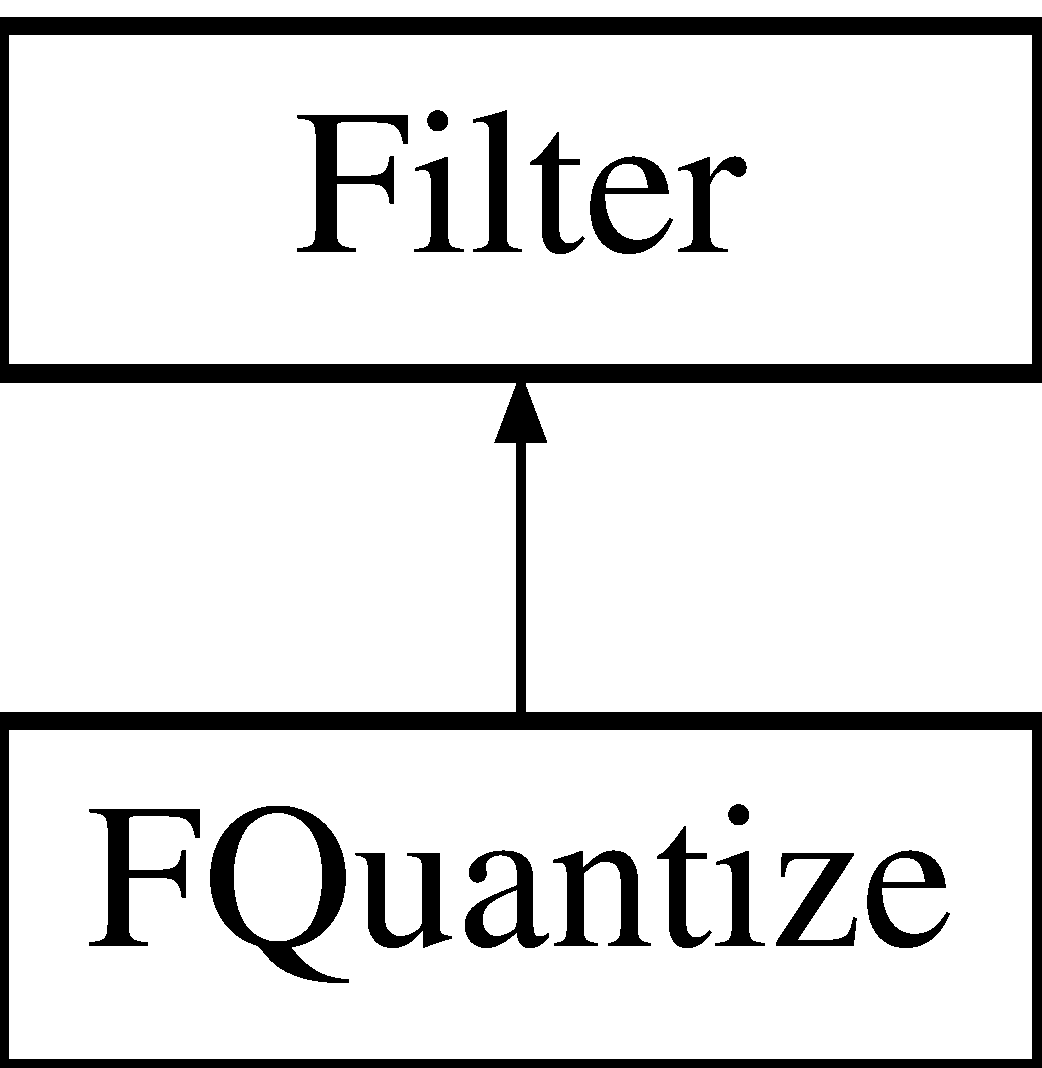
\includegraphics[height=2.000000cm]{classFQuantize}
\end{center}
\end{figure}
\subsection*{Public Member Functions}
\begin{DoxyCompactItemize}
\item 
\hypertarget{classFQuantize_a093d0f34480882da50d994eb4e450c64}{void {\bfseries apply\-Filter} (\hyperlink{classPixelBuffer}{Pixel\-Buffer} $\ast$image\-Buffer)}\label{classFQuantize_a093d0f34480882da50d994eb4e450c64}

\item 
\hypertarget{classFQuantize_a9432e52568e0b7608522569e0a438a1d}{std\-::string {\bfseries get\-Name} ()}\label{classFQuantize_a9432e52568e0b7608522569e0a438a1d}

\item 
\hypertarget{classFQuantize_a093d0f34480882da50d994eb4e450c64}{void {\bfseries apply\-Filter} (\hyperlink{classPixelBuffer}{Pixel\-Buffer} $\ast$image\-Buffer)}\label{classFQuantize_a093d0f34480882da50d994eb4e450c64}

\item 
\hypertarget{classFQuantize_a9432e52568e0b7608522569e0a438a1d}{std\-::string {\bfseries get\-Name} ()}\label{classFQuantize_a9432e52568e0b7608522569e0a438a1d}

\item 
\hypertarget{classFQuantize_a093d0f34480882da50d994eb4e450c64}{void {\bfseries apply\-Filter} (\hyperlink{classPixelBuffer}{Pixel\-Buffer} $\ast$image\-Buffer)}\label{classFQuantize_a093d0f34480882da50d994eb4e450c64}

\item 
\hypertarget{classFQuantize_a9432e52568e0b7608522569e0a438a1d}{std\-::string {\bfseries get\-Name} ()}\label{classFQuantize_a9432e52568e0b7608522569e0a438a1d}

\end{DoxyCompactItemize}


The documentation for this class was generated from the following files\-:\begin{DoxyCompactItemize}
\item 
libphoto/F\-Quantize.\-h\item 
libphoto/include/libphoto.\-h\item 
libphoto/F\-Quantize.\-cpp\end{DoxyCompactItemize}

\hypertarget{classFSaturation}{}\section{F\+Saturation Class Reference}
\label{classFSaturation}\index{F\+Saturation@{F\+Saturation}}
Inheritance diagram for F\+Saturation\+:\begin{figure}[H]
\begin{center}
\leavevmode
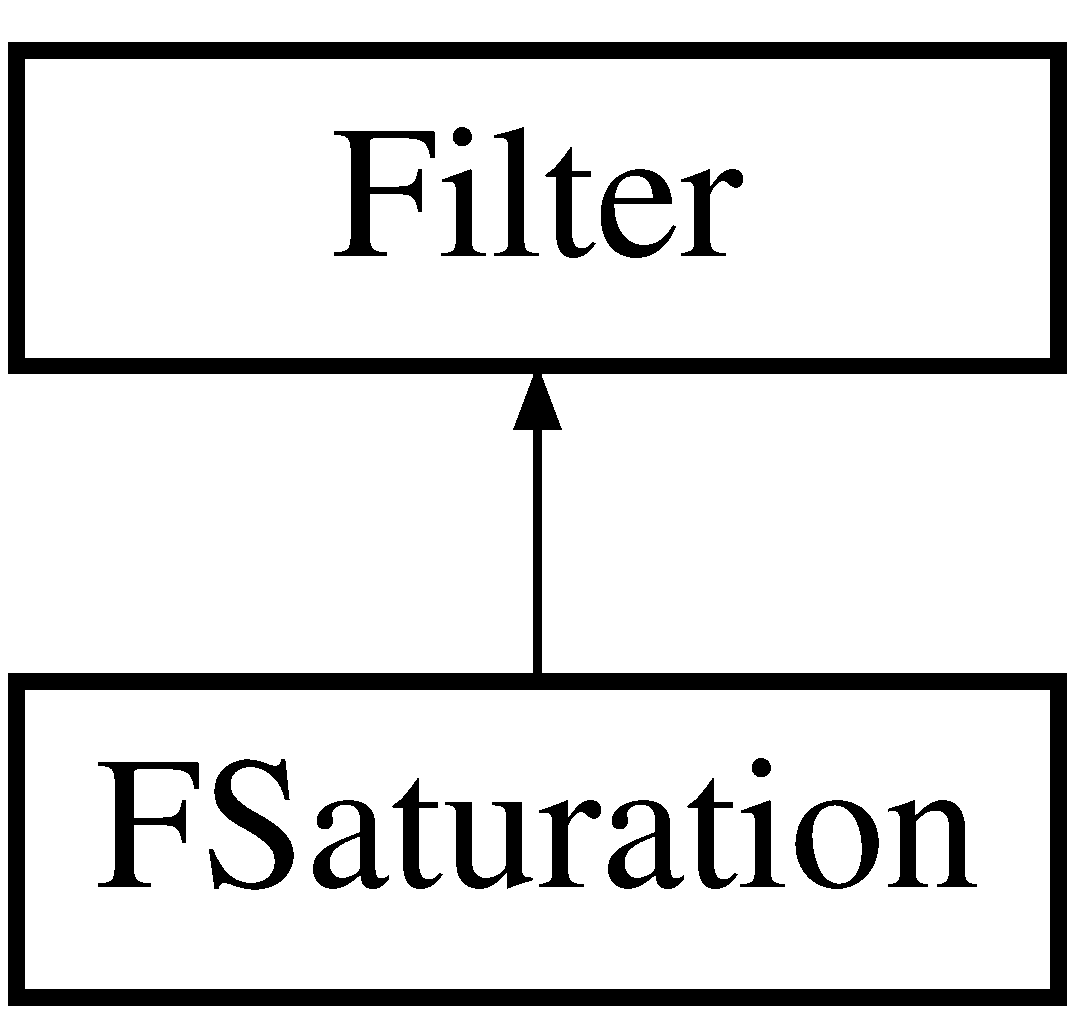
\includegraphics[height=2.000000cm]{classFSaturation}
\end{center}
\end{figure}
\subsection*{Public Member Functions}
\begin{DoxyCompactItemize}
\item 
\hyperlink{classFSaturation_a164678727eb7204e4946578b339617b7}{F\+Saturation} ()
\item 
void \hyperlink{classFSaturation_a9e35fd05500411807bfcbe36b8f24a55}{apply\+Filter} (\hyperlink{classPixelBuffer}{Pixel\+Buffer} $\ast$image\+Buffer)\hypertarget{classFSaturation_a9e35fd05500411807bfcbe36b8f24a55}{}\label{classFSaturation_a9e35fd05500411807bfcbe36b8f24a55}

\begin{DoxyCompactList}\small\item\em apply filter effect to Pixel\+Buffer$\ast$ buffer passed into this function \end{DoxyCompactList}\item 
std\+::string \hyperlink{classFSaturation_a55d272a3a50fcb65d94a66821b7b0c73}{get\+Name} ()\hypertarget{classFSaturation_a55d272a3a50fcb65d94a66821b7b0c73}{}\label{classFSaturation_a55d272a3a50fcb65d94a66821b7b0c73}

\begin{DoxyCompactList}\small\item\em get class name for filter \end{DoxyCompactList}\end{DoxyCompactItemize}


\subsection{Constructor \& Destructor Documentation}
\index{F\+Saturation@{F\+Saturation}!F\+Saturation@{F\+Saturation}}
\index{F\+Saturation@{F\+Saturation}!F\+Saturation@{F\+Saturation}}
\subsubsection[{\texorpdfstring{F\+Saturation()}{FSaturation()}}]{\setlength{\rightskip}{0pt plus 5cm}F\+Saturation\+::\+F\+Saturation (
\begin{DoxyParamCaption}
{}
\end{DoxyParamCaption}
)}\hypertarget{classFSaturation_a164678727eb7204e4946578b339617b7}{}\label{classFSaturation_a164678727eb7204e4946578b339617b7}
This is the \hyperlink{classFSaturation}{F\+Saturation} class, it is used for the saturation image filters. This does not use kernels so it only has to deal with applying the filter 

The documentation for this class was generated from the following files\+:\begin{DoxyCompactItemize}
\item 
libphoto/F\+Saturation.\+h\item 
libphoto/F\+Saturation.\+cpp\end{DoxyCompactItemize}

\hypertarget{classFSharpen}{\section{F\-Sharpen Class Reference}
\label{classFSharpen}\index{F\-Sharpen@{F\-Sharpen}}
}
Inheritance diagram for F\-Sharpen\-:\begin{figure}[H]
\begin{center}
\leavevmode
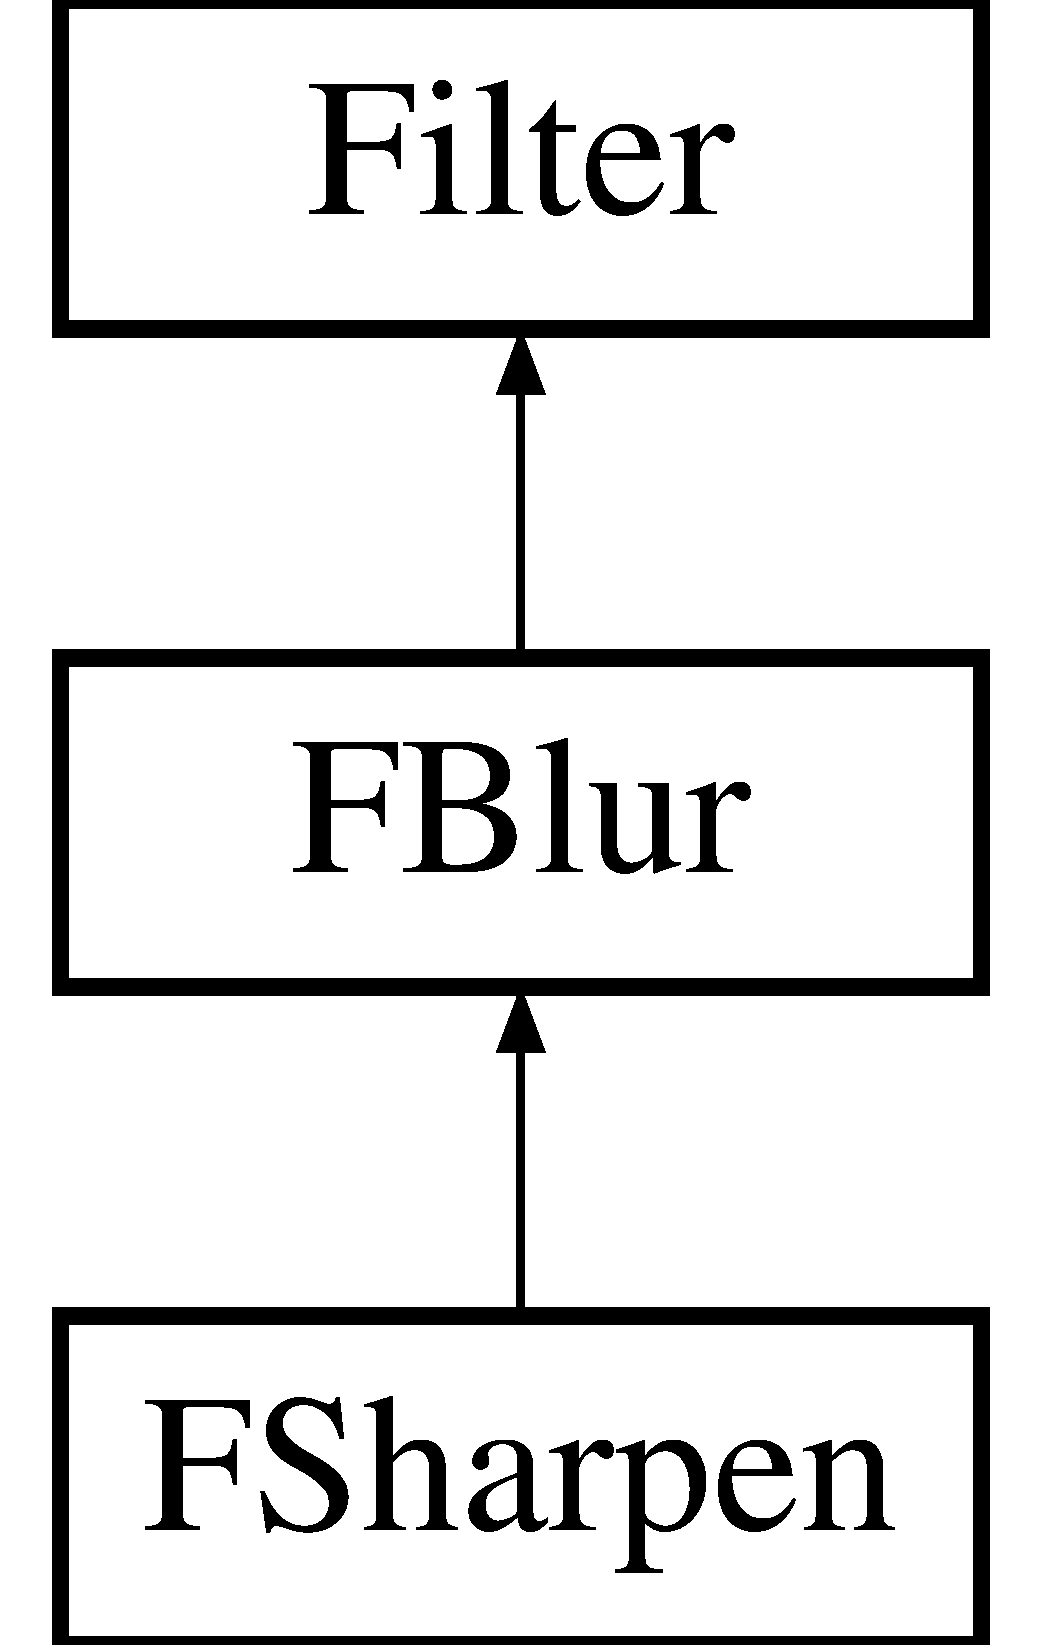
\includegraphics[height=3.000000cm]{classFSharpen}
\end{center}
\end{figure}
\subsection*{Public Member Functions}
\begin{DoxyCompactItemize}
\item 
\hypertarget{classFSharpen_ae322ad5626a003ae1e1c6e385dd43ca8}{std\-::string {\bfseries get\-Name} ()}\label{classFSharpen_ae322ad5626a003ae1e1c6e385dd43ca8}

\item 
\hypertarget{classFSharpen_afafd2b34e58d2fb682150be2159d7986}{kernel\-Type {\bfseries build\-Kernel} (int radius)}\label{classFSharpen_afafd2b34e58d2fb682150be2159d7986}

\end{DoxyCompactItemize}


The documentation for this class was generated from the following files\-:\begin{DoxyCompactItemize}
\item 
libphoto/F\-Sharpen.\-h\item 
libphoto/F\-Sharpen.\-cpp\end{DoxyCompactItemize}

\hypertarget{classFSpecial}{\section{F\-Special Class Reference}
\label{classFSpecial}\index{F\-Special@{F\-Special}}
}
Inheritance diagram for F\-Special\-:\begin{figure}[H]
\begin{center}
\leavevmode
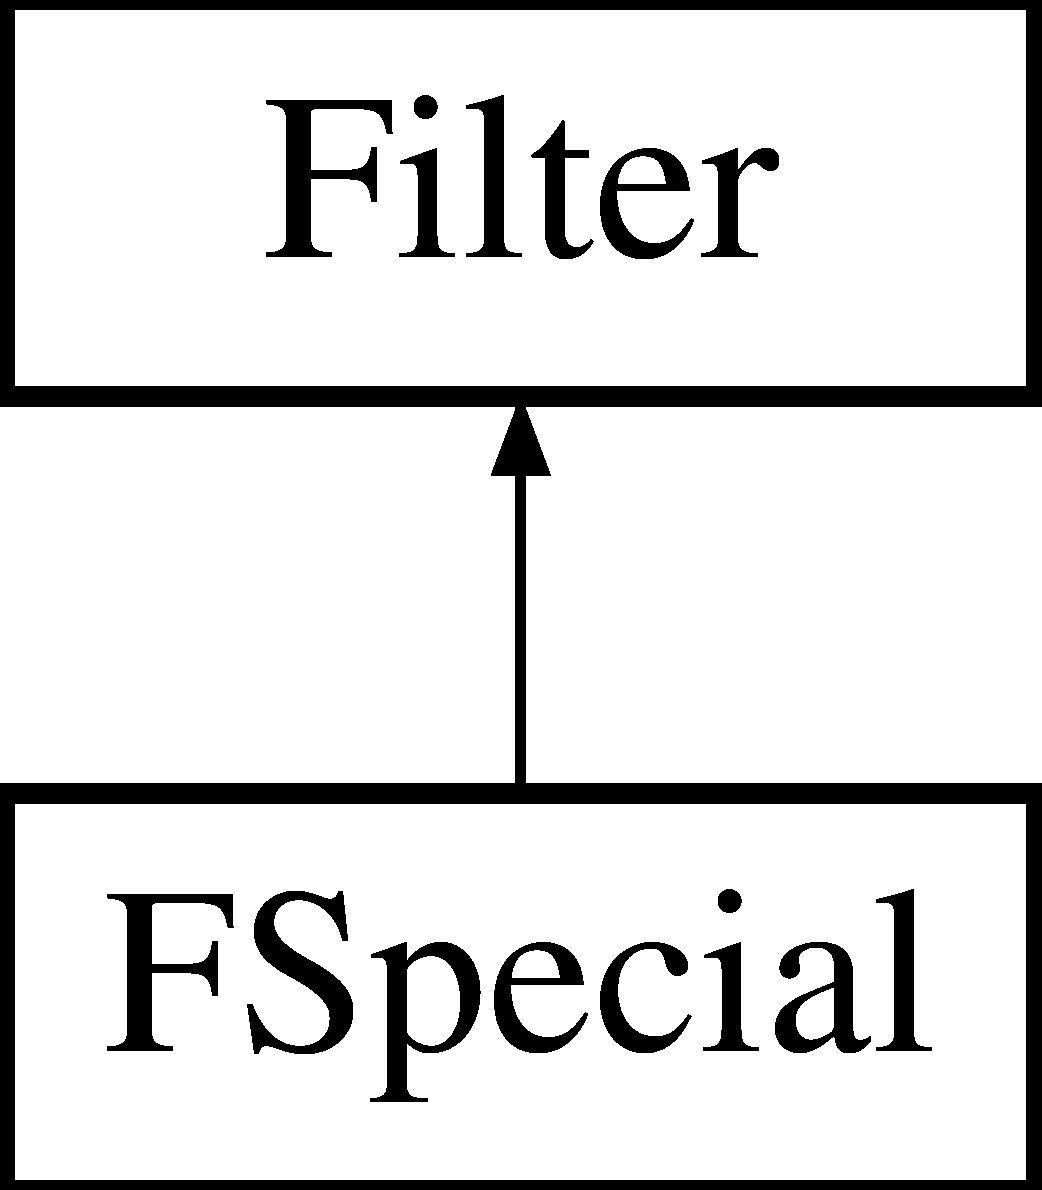
\includegraphics[height=2.000000cm]{classFSpecial}
\end{center}
\end{figure}
\subsection*{Public Member Functions}
\begin{DoxyCompactItemize}
\item 
\hypertarget{classFSpecial_ad5af4242e35da376aeb628e6a7cabc5e}{void {\bfseries apply\-Filter} (\hyperlink{classPixelBuffer}{Pixel\-Buffer} $\ast$image\-Buffer)}\label{classFSpecial_ad5af4242e35da376aeb628e6a7cabc5e}

\item 
\hypertarget{classFSpecial_a769159ff4dc9f6ebd64a6bbe5ae2e917}{std\-::string {\bfseries get\-Name} ()}\label{classFSpecial_a769159ff4dc9f6ebd64a6bbe5ae2e917}

\item 
\hypertarget{classFSpecial_ad5af4242e35da376aeb628e6a7cabc5e}{void {\bfseries apply\-Filter} (\hyperlink{classPixelBuffer}{Pixel\-Buffer} $\ast$image\-Buffer)}\label{classFSpecial_ad5af4242e35da376aeb628e6a7cabc5e}

\item 
\hypertarget{classFSpecial_a769159ff4dc9f6ebd64a6bbe5ae2e917}{std\-::string {\bfseries get\-Name} ()}\label{classFSpecial_a769159ff4dc9f6ebd64a6bbe5ae2e917}

\item 
\hypertarget{classFSpecial_ad5af4242e35da376aeb628e6a7cabc5e}{void {\bfseries apply\-Filter} (\hyperlink{classPixelBuffer}{Pixel\-Buffer} $\ast$image\-Buffer)}\label{classFSpecial_ad5af4242e35da376aeb628e6a7cabc5e}

\item 
\hypertarget{classFSpecial_a769159ff4dc9f6ebd64a6bbe5ae2e917}{std\-::string {\bfseries get\-Name} ()}\label{classFSpecial_a769159ff4dc9f6ebd64a6bbe5ae2e917}

\end{DoxyCompactItemize}


The documentation for this class was generated from the following files\-:\begin{DoxyCompactItemize}
\item 
libphoto/F\-Special.\-h\item 
libphoto/include/libphoto.\-h\item 
libphoto/F\-Special.\-cpp\end{DoxyCompactItemize}

\hypertarget{classFThreshold}{\section{F\-Threshold Class Reference}
\label{classFThreshold}\index{F\-Threshold@{F\-Threshold}}
}
Inheritance diagram for F\-Threshold\-:\begin{figure}[H]
\begin{center}
\leavevmode
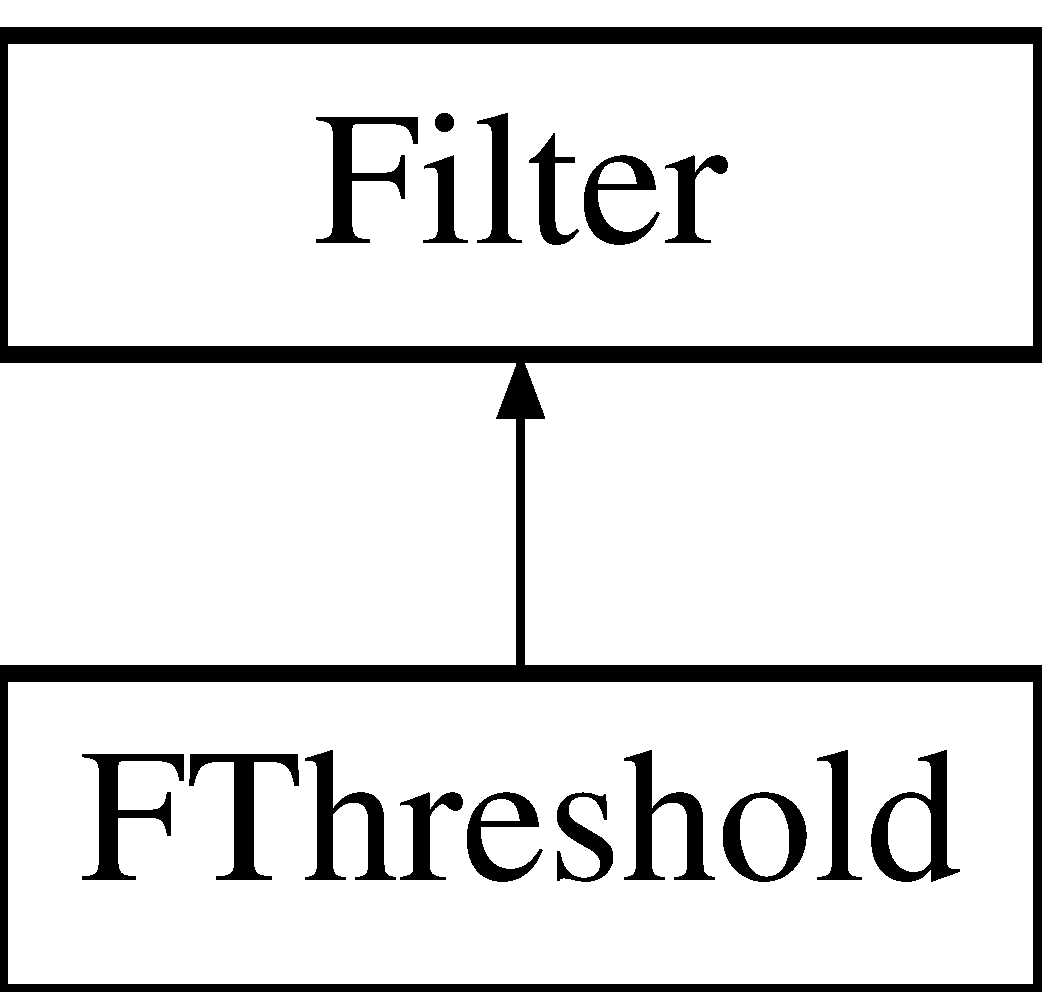
\includegraphics[height=2.000000cm]{classFThreshold}
\end{center}
\end{figure}
\subsection*{Public Member Functions}
\begin{DoxyCompactItemize}
\item 
\hypertarget{classFThreshold_a324dadf15c23bd2d2edf6ea32e3d87f6}{void {\bfseries apply\-Filter} (\hyperlink{classPixelBuffer}{Pixel\-Buffer} $\ast$image\-Buffer)}\label{classFThreshold_a324dadf15c23bd2d2edf6ea32e3d87f6}

\item 
\hypertarget{classFThreshold_a189f8f15c0719706a7eb191b198c0b15}{std\-::string {\bfseries get\-Name} ()}\label{classFThreshold_a189f8f15c0719706a7eb191b198c0b15}

\end{DoxyCompactItemize}


The documentation for this class was generated from the following files\-:\begin{DoxyCompactItemize}
\item 
libphoto/F\-Threshold.\-h\item 
libphoto/F\-Threshold.\-cpp\end{DoxyCompactItemize}

\hypertarget{classHighlighter}{\section{Highlighter Class Reference}
\label{classHighlighter}\index{Highlighter@{Highlighter}}
}
Inheritance diagram for Highlighter\-:\begin{figure}[H]
\begin{center}
\leavevmode
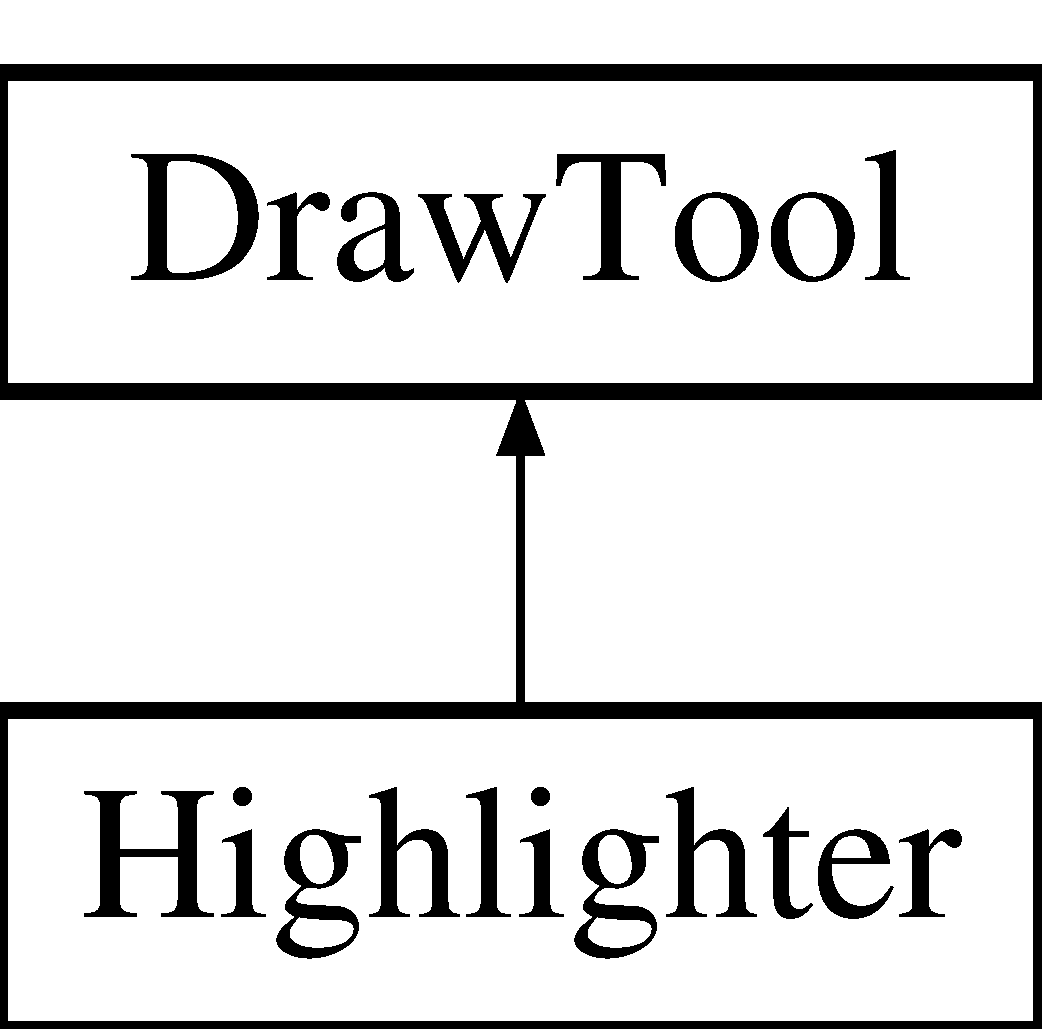
\includegraphics[height=2.000000cm]{classHighlighter}
\end{center}
\end{figure}
\subsection*{Public Member Functions}
\begin{DoxyCompactItemize}
\item 
\hypertarget{classHighlighter_aec9c28167c01f98e3da6eb38e64e6c67}{{\bfseries Highlighter} (\hyperlink{classColorData}{Color\-Data} $\ast$tool\-Color, int width, int height)}\label{classHighlighter_aec9c28167c01f98e3da6eb38e64e6c67}

\item 
\hypertarget{classHighlighter_ab2d858cc3fbddace3f64688293cad8e1}{void {\bfseries fill\-Influence} ()}\label{classHighlighter_ab2d858cc3fbddace3f64688293cad8e1}

\item 
\hypertarget{classHighlighter_a28e750d99d9aa85521427001ef73be0d}{void {\bfseries apply\-Influence} (int x, int y, \hyperlink{classPixelBuffer}{Pixel\-Buffer} $\ast$buffer)}\label{classHighlighter_a28e750d99d9aa85521427001ef73be0d}

\item 
\hypertarget{classHighlighter_aab9bc271db3cc23737e7604a9ab29211}{string {\bfseries get\-Name} ()}\label{classHighlighter_aab9bc271db3cc23737e7604a9ab29211}

\end{DoxyCompactItemize}
\subsection*{Additional Inherited Members}


The documentation for this class was generated from the following files\-:\begin{DoxyCompactItemize}
\item 
libphoto/Highlighter.\-h\item 
libphoto/Highlighter.\-cpp\end{DoxyCompactItemize}

\hypertarget{classImageHandler}{\section{Image\-Handler Class Reference}
\label{classImageHandler}\index{Image\-Handler@{Image\-Handler}}
}
\subsection*{Public Member Functions}
\begin{DoxyCompactItemize}
\item 
\hyperlink{classImageHandler_a86d8324568727c2799a54a43d7296ddb}{Image\-Handler} ()
\item 
\hyperlink{classPixelBuffer}{Pixel\-Buffer} $\ast$ \hyperlink{classImageHandler_a0042244c7f1462f4ffc2403f139bf286}{loadimage} (const std\-::string \&filename, int \&height, int \&width, \hyperlink{classColorData}{Color\-Data} background\-Color)
\item 
void \hyperlink{classImageHandler_ace874907681fc4970f6a2ae2377833b9}{saveimage} (const std\-::string \&filename, \hyperlink{classPixelBuffer}{Pixel\-Buffer} $\ast$buffer)
\end{DoxyCompactItemize}
\subsection*{Private Member Functions}
\begin{DoxyCompactItemize}
\item 
\hypertarget{classImageHandler_acab3c475db0bafa4962e1c368c6c8dab}{bool {\bfseries isjpeg} (const std\-::string \&name)}\label{classImageHandler_acab3c475db0bafa4962e1c368c6c8dab}

\item 
\hypertarget{classImageHandler_a7b60eda1f737592ee903b184210b3b36}{bool {\bfseries ispng} (const std\-::string \&name)}\label{classImageHandler_a7b60eda1f737592ee903b184210b3b36}

\item 
\hypertarget{classImageHandler_a1e2f52b22c7db4f272e715ce41cfb50f}{bool {\bfseries is\-Valid\-Image\-File\-Name} (const std\-::string \&name)}\label{classImageHandler_a1e2f52b22c7db4f272e715ce41cfb50f}

\item 
\hypertarget{classImageHandler_a156a3bd0b6a5381a62863af5d21cf346}{bool {\bfseries is\-Valid\-File} (const std\-::string \&name)}\label{classImageHandler_a156a3bd0b6a5381a62863af5d21cf346}

\item 
\hypertarget{classImageHandler_a00a0f953ebe114ef1925ddafef149354}{bool {\bfseries has\-Suffix} (const std\-::string \&str, const std\-::string \&suffix)}\label{classImageHandler_a00a0f953ebe114ef1925ddafef149354}

\item 
void \hyperlink{classImageHandler_afa5073aef96331be8b7c3e8fe8fbd373}{savepng} (const std\-::string file\-Name, int height, int width, \hyperlink{classPixelBuffer}{Pixel\-Buffer} $\ast$buffer)
\item 
void \hyperlink{classImageHandler_a93c1210df4b0b9d673e3ba99f1452d60}{savejpg} (F\-I\-L\-E $\ast$infile, int height, int width, \hyperlink{classPixelBuffer}{Pixel\-Buffer} $\ast$buffer)
\item 
\hyperlink{classPixelBuffer}{Pixel\-Buffer} $\ast$ \hyperlink{classImageHandler_a0812c8e895f28203138d8e67f3be2418}{loadpng} (const std\-::string file\-Name, int \&height, int \&width, \hyperlink{classColorData}{Color\-Data} background\-Color)
\item 
\hyperlink{classPixelBuffer}{Pixel\-Buffer} $\ast$ \hyperlink{classImageHandler_a84ff67cb9c77f69cf3a66bdcd4e3f977}{loadjpg} (F\-I\-L\-E $\ast$infile, int \&height, int \&width, \hyperlink{classColorData}{Color\-Data} background\-Color)
\end{DoxyCompactItemize}


\subsection{Constructor \& Destructor Documentation}
\hypertarget{classImageHandler_a86d8324568727c2799a54a43d7296ddb}{\index{Image\-Handler@{Image\-Handler}!Image\-Handler@{Image\-Handler}}
\index{Image\-Handler@{Image\-Handler}!ImageHandler@{Image\-Handler}}
\subsubsection[{Image\-Handler}]{\setlength{\rightskip}{0pt plus 5cm}Image\-Handler\-::\-Image\-Handler (
\begin{DoxyParamCaption}
{}
\end{DoxyParamCaption}
)}}\label{classImageHandler_a86d8324568727c2799a54a43d7296ddb}
This is the \hyperlink{classImageHandler}{Image\-Handler} class. This contains all of the logic for saving/loading jpegs/pngs. 

\subsection{Member Function Documentation}
\hypertarget{classImageHandler_a0042244c7f1462f4ffc2403f139bf286}{\index{Image\-Handler@{Image\-Handler}!loadimage@{loadimage}}
\index{loadimage@{loadimage}!ImageHandler@{Image\-Handler}}
\subsubsection[{loadimage}]{\setlength{\rightskip}{0pt plus 5cm}{\bf Pixel\-Buffer} $\ast$ Image\-Handler\-::loadimage (
\begin{DoxyParamCaption}
\item[{const std\-::string \&}]{filename, }
\item[{int \&}]{height, }
\item[{int \&}]{width, }
\item[{{\bf Color\-Data}}]{background\-Color}
\end{DoxyParamCaption}
)}}\label{classImageHandler_a0042244c7f1462f4ffc2403f139bf286}
Load an image in to the pixel buffer \par
filename, height reference, width reference \par
The pixel buffer with the image loaded \par
\hypertarget{classImageHandler_a84ff67cb9c77f69cf3a66bdcd4e3f977}{\index{Image\-Handler@{Image\-Handler}!loadjpg@{loadjpg}}
\index{loadjpg@{loadjpg}!ImageHandler@{Image\-Handler}}
\subsubsection[{loadjpg}]{\setlength{\rightskip}{0pt plus 5cm}{\bf Pixel\-Buffer} $\ast$ Image\-Handler\-::loadjpg (
\begin{DoxyParamCaption}
\item[{F\-I\-L\-E $\ast$}]{infile, }
\item[{int \&}]{Height, }
\item[{int \&}]{Width, }
\item[{{\bf Color\-Data}}]{background\-Color}
\end{DoxyParamCaption}
)\hspace{0.3cm}{\ttfamily [private]}}}\label{classImageHandler_a84ff67cb9c77f69cf3a66bdcd4e3f977}
Load a jpg from the file \par
file pointer, height of image, width of image \par
\hyperlink{classPixelBuffer}{Pixel\-Buffer} containing the image \par
\hypertarget{classImageHandler_a0812c8e895f28203138d8e67f3be2418}{\index{Image\-Handler@{Image\-Handler}!loadpng@{loadpng}}
\index{loadpng@{loadpng}!ImageHandler@{Image\-Handler}}
\subsubsection[{loadpng}]{\setlength{\rightskip}{0pt plus 5cm}{\bf Pixel\-Buffer} $\ast$ Image\-Handler\-::loadpng (
\begin{DoxyParamCaption}
\item[{const std\-::string}]{file\-Name, }
\item[{int \&}]{Height, }
\item[{int \&}]{Width, }
\item[{{\bf Color\-Data}}]{background\-Color}
\end{DoxyParamCaption}
)\hspace{0.3cm}{\ttfamily [private]}}}\label{classImageHandler_a0812c8e895f28203138d8e67f3be2418}
Load a png from the file \par
file pointer, height of image, width of image \par
\hyperlink{classPixelBuffer}{Pixel\-Buffer} containing the image \par
\hypertarget{classImageHandler_ace874907681fc4970f6a2ae2377833b9}{\index{Image\-Handler@{Image\-Handler}!saveimage@{saveimage}}
\index{saveimage@{saveimage}!ImageHandler@{Image\-Handler}}
\subsubsection[{saveimage}]{\setlength{\rightskip}{0pt plus 5cm}void Image\-Handler\-::saveimage (
\begin{DoxyParamCaption}
\item[{const std\-::string \&}]{filename, }
\item[{{\bf Pixel\-Buffer} $\ast$}]{buffer}
\end{DoxyParamCaption}
)}}\label{classImageHandler_ace874907681fc4970f6a2ae2377833b9}
Save an image to the file \par
filename, height of image, width of image, image \par
void \par
\hypertarget{classImageHandler_a93c1210df4b0b9d673e3ba99f1452d60}{\index{Image\-Handler@{Image\-Handler}!savejpg@{savejpg}}
\index{savejpg@{savejpg}!ImageHandler@{Image\-Handler}}
\subsubsection[{savejpg}]{\setlength{\rightskip}{0pt plus 5cm}void Image\-Handler\-::savejpg (
\begin{DoxyParamCaption}
\item[{F\-I\-L\-E $\ast$}]{outfile, }
\item[{int}]{Height, }
\item[{int}]{Width, }
\item[{{\bf Pixel\-Buffer} $\ast$}]{buffer\-To\-Save}
\end{DoxyParamCaption}
)\hspace{0.3cm}{\ttfamily [private]}}}\label{classImageHandler_a93c1210df4b0b9d673e3ba99f1452d60}
save a jpg to the file \par
file pointer, height of image, width of image, image \par
void \par
\hypertarget{classImageHandler_afa5073aef96331be8b7c3e8fe8fbd373}{\index{Image\-Handler@{Image\-Handler}!savepng@{savepng}}
\index{savepng@{savepng}!ImageHandler@{Image\-Handler}}
\subsubsection[{savepng}]{\setlength{\rightskip}{0pt plus 5cm}void Image\-Handler\-::savepng (
\begin{DoxyParamCaption}
\item[{const std\-::string}]{file\-Name, }
\item[{int}]{height, }
\item[{int}]{width, }
\item[{{\bf Pixel\-Buffer} $\ast$}]{buffer\-To\-Save}
\end{DoxyParamCaption}
)\hspace{0.3cm}{\ttfamily [private]}}}\label{classImageHandler_afa5073aef96331be8b7c3e8fe8fbd373}
Save a png to the file \par
file pointer, height of image, width of image, image \par
void \par


The documentation for this class was generated from the following files\-:\begin{DoxyCompactItemize}
\item 
libphoto/Image\-Handler.\-h\item 
libphoto/Image\-Handler.\-cpp\end{DoxyCompactItemize}

\hypertarget{classMask}{\section{Mask Class Reference}
\label{classMask}\index{Mask@{Mask}}
}
\subsection*{Public Member Functions}
\begin{DoxyCompactItemize}
\item 
\hyperlink{classMask_a1fdc1ca0927f8f6b792cc3130087f933}{Mask} (int w, int h)
\item 
int \hyperlink{classMask_a38d79e2785ddb9b1684b1183963091af}{get\-Height} () const 
\item 
int \hyperlink{classMask_a3367b822da66a059ac6f16e79472566f}{get\-Width} () const 
\item 
float $\ast$$\ast$ \hyperlink{classMask_a5a7cfb7560ca289748040963b64f91ae}{get\-Influence} () const 
\end{DoxyCompactItemize}
\subsection*{Protected Attributes}
\begin{DoxyCompactItemize}
\item 
\hypertarget{classMask_ae5fec5d187fb0fc64383badbbd5773d4}{int {\bfseries height}}\label{classMask_ae5fec5d187fb0fc64383badbbd5773d4}

\item 
\hypertarget{classMask_a3bf4b8e804ee6ba93e0e62a71062fa1e}{int {\bfseries width}}\label{classMask_a3bf4b8e804ee6ba93e0e62a71062fa1e}

\item 
\hypertarget{classMask_a0d551850a8c005e17070e31666f0c0d0}{float $\ast$$\ast$ {\bfseries influence}}\label{classMask_a0d551850a8c005e17070e31666f0c0d0}

\end{DoxyCompactItemize}


\subsection{Constructor \& Destructor Documentation}
\hypertarget{classMask_a1fdc1ca0927f8f6b792cc3130087f933}{\index{Mask@{Mask}!Mask@{Mask}}
\index{Mask@{Mask}!Mask@{Mask}}
\subsubsection[{Mask}]{\setlength{\rightskip}{0pt plus 5cm}Mask\-::\-Mask (
\begin{DoxyParamCaption}
\item[{int}]{w, }
\item[{int}]{h}
\end{DoxyParamCaption}
)}}\label{classMask_a1fdc1ca0927f8f6b792cc3130087f933}
This is the mask class. This describes the basic format for our Draw\-Tools. Every drawtool should have a mask 

\subsection{Member Function Documentation}
\hypertarget{classMask_a38d79e2785ddb9b1684b1183963091af}{\index{Mask@{Mask}!get\-Height@{get\-Height}}
\index{get\-Height@{get\-Height}!Mask@{Mask}}
\subsubsection[{get\-Height}]{\setlength{\rightskip}{0pt plus 5cm}int Mask\-::get\-Height (
\begin{DoxyParamCaption}
{}
\end{DoxyParamCaption}
) const}}\label{classMask_a38d79e2785ddb9b1684b1183963091af}
Get the height of the mask \par
 none \par
 returns the height of the mask \par
\hypertarget{classMask_a5a7cfb7560ca289748040963b64f91ae}{\index{Mask@{Mask}!get\-Influence@{get\-Influence}}
\index{get\-Influence@{get\-Influence}!Mask@{Mask}}
\subsubsection[{get\-Influence}]{\setlength{\rightskip}{0pt plus 5cm}float $\ast$$\ast$ Mask\-::get\-Influence (
\begin{DoxyParamCaption}
{}
\end{DoxyParamCaption}
) const}}\label{classMask_a5a7cfb7560ca289748040963b64f91ae}
Get the influence array of the mask \par
 none \par
 returns a pointer to the array of influence for the mask \par
\hypertarget{classMask_a3367b822da66a059ac6f16e79472566f}{\index{Mask@{Mask}!get\-Width@{get\-Width}}
\index{get\-Width@{get\-Width}!Mask@{Mask}}
\subsubsection[{get\-Width}]{\setlength{\rightskip}{0pt plus 5cm}int Mask\-::get\-Width (
\begin{DoxyParamCaption}
{}
\end{DoxyParamCaption}
) const}}\label{classMask_a3367b822da66a059ac6f16e79472566f}
Get the width of the mask \par
 none \par
 returns the width of the mask \par


The documentation for this class was generated from the following files\-:\begin{DoxyCompactItemize}
\item 
libphoto/Mask.\-h\item 
libphoto/Mask.\-cpp\end{DoxyCompactItemize}

\hypertarget{classMIAApp}{\section{M\-I\-A\-App Class Reference}
\label{classMIAApp}\index{M\-I\-A\-App@{M\-I\-A\-App}}
}
Inheritance diagram for M\-I\-A\-App\-:\begin{figure}[H]
\begin{center}
\leavevmode
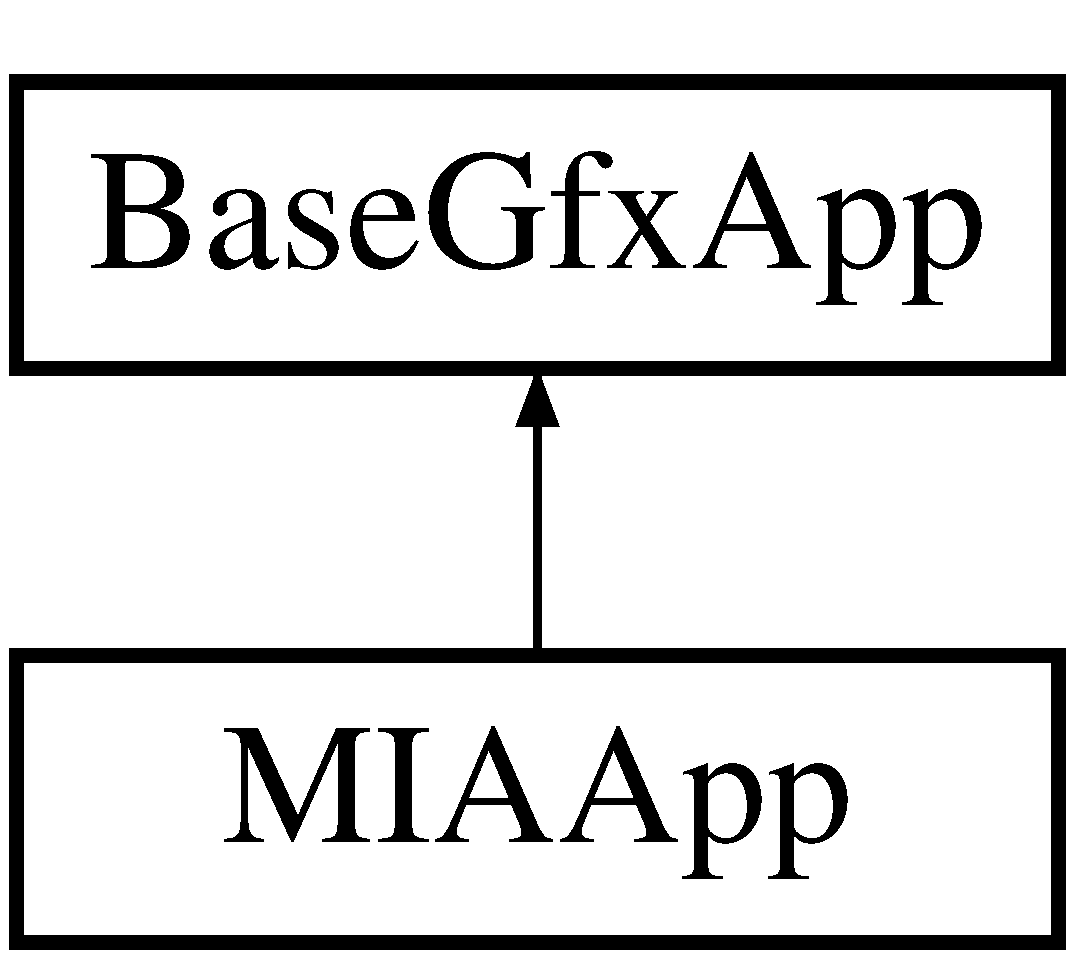
\includegraphics[height=2.000000cm]{classMIAApp}
\end{center}
\end{figure}
\subsection*{Public Member Functions}
\begin{DoxyCompactItemize}
\item 
\hypertarget{classMIAApp_a99c82819221bee486f5eb1628df3dc58}{{\bfseries M\-I\-A\-App} (int argc, char $\ast$argv\mbox{[}$\,$\mbox{]})}\label{classMIAApp_a99c82819221bee486f5eb1628df3dc58}

\item 
\hypertarget{classMIAApp_a0dbcbcd31a2ba7fd55988354e9cc0d93}{{\bfseries M\-I\-A\-App} (int argc, char $\ast$argv\mbox{[}$\,$\mbox{]}, int width, int height, \hyperlink{classColorData}{Color\-Data} background\-Color)}\label{classMIAApp_a0dbcbcd31a2ba7fd55988354e9cc0d93}

\item 
\hypertarget{classMIAApp_a92f074cdaf7660abf7da902ad78f7ceb}{void {\bfseries mouse\-Dragged} (int x, int y)}\label{classMIAApp_a92f074cdaf7660abf7da902ad78f7ceb}

\item 
\hypertarget{classMIAApp_a89342bccfdad6cd476677f19edf7c9bd}{void {\bfseries mouse\-Moved} (int x, int y)}\label{classMIAApp_a89342bccfdad6cd476677f19edf7c9bd}

\item 
\hypertarget{classMIAApp_a8174b71f6537aea41c1cda099e47a0d0}{void {\bfseries left\-Mouse\-Down} (int x, int y)}\label{classMIAApp_a8174b71f6537aea41c1cda099e47a0d0}

\item 
\hypertarget{classMIAApp_a804a0a6a7e3f165adea88bb416232803}{void {\bfseries left\-Mouse\-Up} (int x, int y)}\label{classMIAApp_a804a0a6a7e3f165adea88bb416232803}

\item 
\hypertarget{classMIAApp_a5b88636a4d17872ab922a4b088696608}{void {\bfseries display} ()}\label{classMIAApp_a5b88636a4d17872ab922a4b088696608}

\item 
\hypertarget{classMIAApp_affee3adfef9a7491607d93554a2bb9c0}{void {\bfseries glui\-Control} (int control\-I\-D)}\label{classMIAApp_affee3adfef9a7491607d93554a2bb9c0}

\end{DoxyCompactItemize}
\subsection*{Additional Inherited Members}


The documentation for this class was generated from the following files\-:\begin{DoxyCompactItemize}
\item 
Mia/M\-I\-A\-App.\-h\item 
Mia/M\-I\-A\-App.\-cpp\end{DoxyCompactItemize}

\hypertarget{classMIACommandLineApp}{\section{M\-I\-A\-Command\-Line\-App Class Reference}
\label{classMIACommandLineApp}\index{M\-I\-A\-Command\-Line\-App@{M\-I\-A\-Command\-Line\-App}}
}
\subsection*{Public Member Functions}
\begin{DoxyCompactItemize}
\item 
\hypertarget{classMIACommandLineApp_a769f7b7b3f3684686afb424c00db4ee4}{\hyperlink{classPixelBuffer}{Pixel\-Buffer} $\ast$ {\bfseries read\-File} (string file)}\label{classMIACommandLineApp_a769f7b7b3f3684686afb424c00db4ee4}

\item 
\hypertarget{classMIACommandLineApp_a5c98945cdad816e6645dc09f1537fc9e}{void {\bfseries write\-File} (string file)}\label{classMIACommandLineApp_a5c98945cdad816e6645dc09f1537fc9e}

\item 
\hypertarget{classMIACommandLineApp_ad7e4e22804b01321b8366627297d3915}{void {\bfseries handle\-Edge\-Detect} ()}\label{classMIACommandLineApp_ad7e4e22804b01321b8366627297d3915}

\item 
\hypertarget{classMIACommandLineApp_a9be162f864792a003931a33d24e1fa52}{void {\bfseries handle\-Blur} (float parameter)}\label{classMIACommandLineApp_a9be162f864792a003931a33d24e1fa52}

\item 
\hypertarget{classMIACommandLineApp_a3a3cd95334889d1c5ae8f0871080bd18}{void {\bfseries handle\-Satur} (float parameter)}\label{classMIACommandLineApp_a3a3cd95334889d1c5ae8f0871080bd18}

\item 
\hypertarget{classMIACommandLineApp_a80568f718b9ed0d0b520cc5f1fb72ca0}{void {\bfseries handle\-Thresh} (float parameter)}\label{classMIACommandLineApp_a80568f718b9ed0d0b520cc5f1fb72ca0}

\item 
\hypertarget{classMIACommandLineApp_ae231f6b1b186a3f4ae7d168175e7fac4}{void {\bfseries handle\-Sharpen} (int parameter)}\label{classMIACommandLineApp_ae231f6b1b186a3f4ae7d168175e7fac4}

\item 
\hypertarget{classMIACommandLineApp_afc01f09633833fa92beedb52f2098ca7}{int {\bfseries handle\-Compare} (string input, string ouput)}\label{classMIACommandLineApp_afc01f09633833fa92beedb52f2098ca7}

\item 
\hypertarget{classMIACommandLineApp_ab3837792e96c27534b0290e7b7bdd5cc}{void {\bfseries handle\-Multgb} (\hyperlink{classColorData}{Color\-Data} color)}\label{classMIACommandLineApp_ab3837792e96c27534b0290e7b7bdd5cc}

\item 
\hypertarget{classMIACommandLineApp_a7dd611671ab000d8c7975d4b9b2f125b}{void {\bfseries handle\-Quant} (int parameter)}\label{classMIACommandLineApp_a7dd611671ab000d8c7975d4b9b2f125b}

\end{DoxyCompactItemize}
\subsection*{Private Attributes}
\begin{DoxyCompactItemize}
\item 
\hypertarget{classMIACommandLineApp_ab0b3fcdb2414478c081d4713f99863c5}{\hyperlink{classPixelBuffer}{Pixel\-Buffer} $\ast$ {\bfseries m\-\_\-buffer}}\label{classMIACommandLineApp_ab0b3fcdb2414478c081d4713f99863c5}

\item 
\hypertarget{classMIACommandLineApp_a193cb889437a249d9517fea6c4ba8140}{\hyperlink{classImageHandler}{Image\-Handler} $\ast$ {\bfseries m\-\_\-loader}}\label{classMIACommandLineApp_a193cb889437a249d9517fea6c4ba8140}

\end{DoxyCompactItemize}


The documentation for this class was generated from the following files\-:\begin{DoxyCompactItemize}
\item 
Mia/M\-I\-A\-Command\-Line\-App.\-h\item 
Mia/M\-I\-A\-Command\-Line\-App.\-cpp\end{DoxyCompactItemize}

\hypertarget{classPen}{\section{Pen Class Reference}
\label{classPen}\index{Pen@{Pen}}
}
Inheritance diagram for Pen\-:\begin{figure}[H]
\begin{center}
\leavevmode
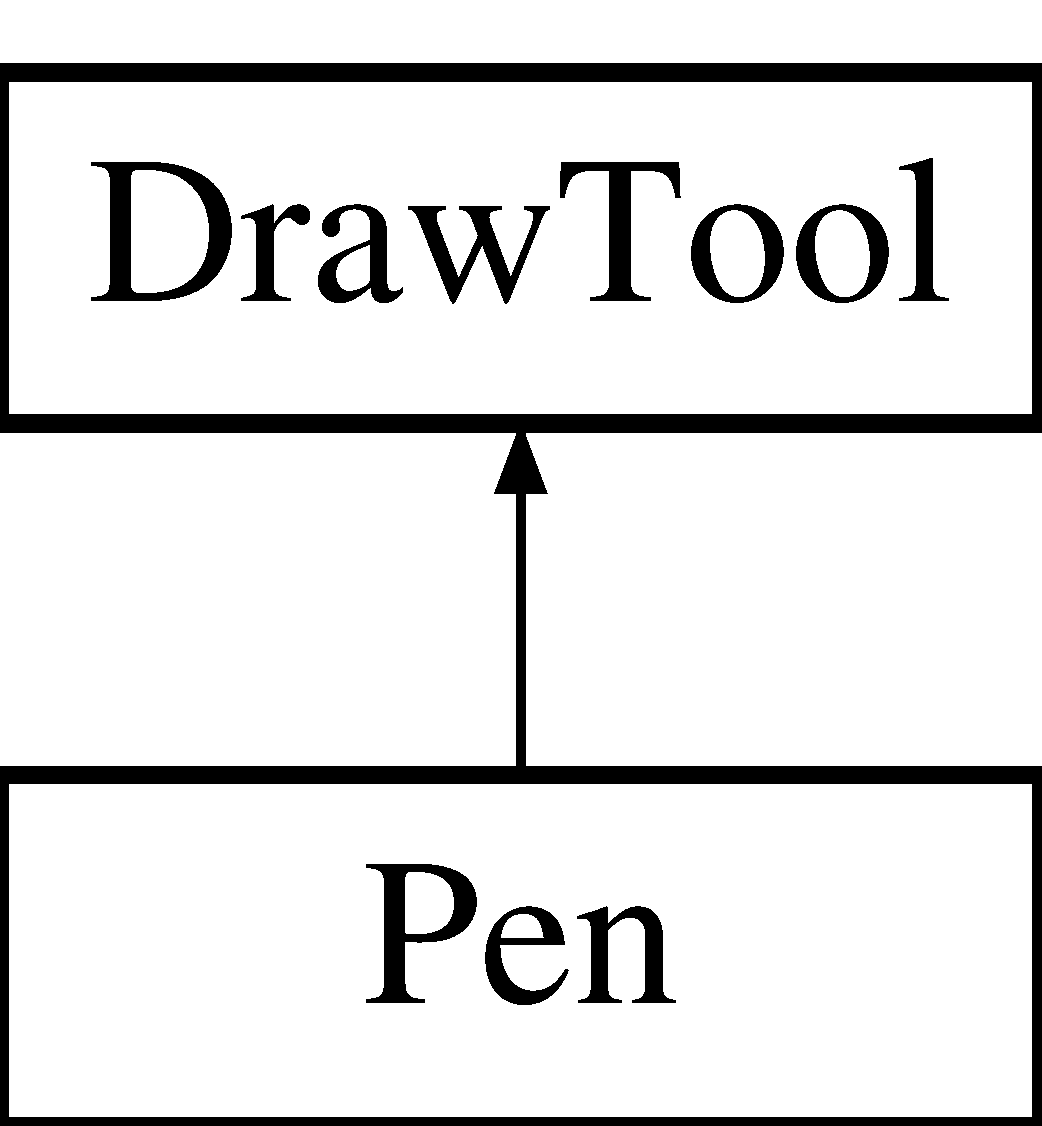
\includegraphics[height=2.000000cm]{classPen}
\end{center}
\end{figure}
\subsection*{Public Member Functions}
\begin{DoxyCompactItemize}
\item 
\hypertarget{classPen_aae1e2ae7aead4ede7484af6554fd93d7}{{\bfseries Pen} (\hyperlink{classColorData}{Color\-Data} $\ast$tool\-Color, int radius)}\label{classPen_aae1e2ae7aead4ede7484af6554fd93d7}

\item 
\hyperlink{classPen_a6c57ef2ef6c352e676bcf77239315605}{$\sim$\-Pen} ()
\begin{DoxyCompactList}\small\item\em For function descriptions please see the \hyperlink{classBlur}{Blur} class. \end{DoxyCompactList}\item 
void \hyperlink{classPen_a3a09d9bed4cefec347fb4dd759faf44a}{fill\-Influence} ()
\item 
\hypertarget{classPen_afece6e7d7f6e22da50d45c585a7ad6b2}{string {\bfseries get\-Name} ()}\label{classPen_afece6e7d7f6e22da50d45c585a7ad6b2}

\end{DoxyCompactItemize}
\subsection*{Additional Inherited Members}


\subsection{Constructor \& Destructor Documentation}
\hypertarget{classPen_a6c57ef2ef6c352e676bcf77239315605}{\index{Pen@{Pen}!$\sim$\-Pen@{$\sim$\-Pen}}
\index{$\sim$\-Pen@{$\sim$\-Pen}!Pen@{Pen}}
\subsubsection[{$\sim$\-Pen}]{\setlength{\rightskip}{0pt plus 5cm}Pen\-::$\sim$\-Pen (
\begin{DoxyParamCaption}
{}
\end{DoxyParamCaption}
)}}\label{classPen_a6c57ef2ef6c352e676bcf77239315605}


For function descriptions please see the \hyperlink{classBlur}{Blur} class. 

This is the pen class. It inherits from the \hyperlink{classDrawTool}{Draw\-Tool} and only needs to deal with loading the influence matrix. \hyperlink{classDrawTool}{Draw\-Tool} applies the influence. 

\subsection{Member Function Documentation}
\hypertarget{classPen_a3a09d9bed4cefec347fb4dd759faf44a}{\index{Pen@{Pen}!fill\-Influence@{fill\-Influence}}
\index{fill\-Influence@{fill\-Influence}!Pen@{Pen}}
\subsubsection[{fill\-Influence}]{\setlength{\rightskip}{0pt plus 5cm}void Pen\-::fill\-Influence (
\begin{DoxyParamCaption}
{}
\end{DoxyParamCaption}
)\hspace{0.3cm}{\ttfamily [virtual]}}}\label{classPen_a3a09d9bed4cefec347fb4dd759faf44a}
Virtual function to set influence on the mask, should be overrode in sub class \par
 none \par
 void \par


Reimplemented from \hyperlink{classDrawTool_ae202bc193ba721452e81f34b6c2e6e35}{Draw\-Tool}.



The documentation for this class was generated from the following files\-:\begin{DoxyCompactItemize}
\item 
libphoto/Pen.\-h\item 
libphoto/Pen.\-cpp\end{DoxyCompactItemize}

\hypertarget{classPixelBuffer}{}\section{Pixel\+Buffer Class Reference}
\label{classPixelBuffer}\index{Pixel\+Buffer@{Pixel\+Buffer}}


{\ttfamily \#include $<$Pixel\+Buffer.\+h$>$}

\subsection*{Public Member Functions}
\begin{DoxyCompactItemize}
\item 
\hyperlink{classPixelBuffer_ae373904fcdd3c820677b959354b75410}{Pixel\+Buffer} (int w, int h, \hyperlink{classColorData}{Color\+Data} background\+Color)
\item 
void \hyperlink{classPixelBuffer_abe673364dfceec95783e1dfb00ec9bd1}{set\+Pixel} (int x, int y, const \hyperlink{classColorData}{Color\+Data} \&color)\hypertarget{classPixelBuffer_abe673364dfceec95783e1dfb00ec9bd1}{}\label{classPixelBuffer_abe673364dfceec95783e1dfb00ec9bd1}

\begin{DoxyCompactList}\small\item\em Set the pixel at the x and y coordinates to the new\+Pixel value. \end{DoxyCompactList}\item 
void {\bfseries fill\+Pixel\+Buffer\+With\+Color} (\hyperlink{classColorData}{Color\+Data} color)\hypertarget{classPixelBuffer_a1bdab74553ab7d569629a42a808b4785}{}\label{classPixelBuffer_a1bdab74553ab7d569629a42a808b4785}

\item 
void {\bfseries convert\+To\+Luminance} ()\hypertarget{classPixelBuffer_a73f0518c147ad7900a64b4ffa205b9fc}{}\label{classPixelBuffer_a73f0518c147ad7900a64b4ffa205b9fc}

\item 
\hyperlink{classColorData}{Color\+Data} \hyperlink{classPixelBuffer_ae01450fb4e9824c1e93e92f4377e9924}{get\+Pixel} (int x, int y) const \hypertarget{classPixelBuffer_ae01450fb4e9824c1e93e92f4377e9924}{}\label{classPixelBuffer_ae01450fb4e9824c1e93e92f4377e9924}

\begin{DoxyCompactList}\small\item\em Get the pixel at the x and y coordinates. \end{DoxyCompactList}\item 
\hyperlink{classColorData}{Color\+Data} const $\ast$ \hyperlink{classPixelBuffer_a4b9ebe9181f451aa7c9858e400245e73}{get\+Data} () const \hypertarget{classPixelBuffer_a4b9ebe9181f451aa7c9858e400245e73}{}\label{classPixelBuffer_a4b9ebe9181f451aa7c9858e400245e73}

\begin{DoxyCompactList}\small\item\em Get the pixel array. \end{DoxyCompactList}\item 
\hyperlink{classColorData}{Color\+Data} {\bfseries get\+Background\+Color} ()\hypertarget{classPixelBuffer_a7eadc0d458fec5d0e0f502d279b86ea7}{}\label{classPixelBuffer_a7eadc0d458fec5d0e0f502d279b86ea7}

\item 
\hyperlink{classColorData}{Color\+Data} {\bfseries get\+Default\+Background\+Color} ()\hypertarget{classPixelBuffer_a36649accdea429915280ba71a7976300}{}\label{classPixelBuffer_a36649accdea429915280ba71a7976300}

\item 
int {\bfseries get\+Height} () const \hypertarget{classPixelBuffer_abd5685a6a23041ed9640da9370eb7839}{}\label{classPixelBuffer_abd5685a6a23041ed9640da9370eb7839}

\item 
int {\bfseries get\+Width} () const \hypertarget{classPixelBuffer_a26dc9286596d27cd416d34611c00602e}{}\label{classPixelBuffer_a26dc9286596d27cd416d34611c00602e}

\item 
void {\bfseries set\+Background\+Color} (\hyperlink{classColorData}{Color\+Data} $\ast$color)\hypertarget{classPixelBuffer_a1838bd976c9c98a79b0c2eb1246b816f}{}\label{classPixelBuffer_a1838bd976c9c98a79b0c2eb1246b816f}

\end{DoxyCompactItemize}
\subsection*{Static Public Member Functions}
\begin{DoxyCompactItemize}
\item 
static void {\bfseries copy\+Pixel\+Buffer} (\hyperlink{classPixelBuffer}{Pixel\+Buffer} $\ast$source\+Buffer, \hyperlink{classPixelBuffer}{Pixel\+Buffer} $\ast$destination\+Buffer)\hypertarget{classPixelBuffer_afedcf4028903278e8eacbd78d11232ee}{}\label{classPixelBuffer_afedcf4028903278e8eacbd78d11232ee}

\item 
static void {\bfseries copy\+Pixel\+Buffer} (\hyperlink{classPixelBuffer}{Pixel\+Buffer} source\+Buffer, \hyperlink{classPixelBuffer}{Pixel\+Buffer} $\ast$destination\+Buffer)\hypertarget{classPixelBuffer_a91bfa4c461b467c0504601a7bc6e29b2}{}\label{classPixelBuffer_a91bfa4c461b467c0504601a7bc6e29b2}

\end{DoxyCompactItemize}
\subsection*{Private Attributes}
\begin{DoxyCompactItemize}
\item 
\hyperlink{classColorData}{Color\+Data} $\ast$ {\bfseries m\+\_\+pixels}\hypertarget{classPixelBuffer_abea92f97fac02c482e18497b71581e58}{}\label{classPixelBuffer_abea92f97fac02c482e18497b71581e58}

\item 
\hyperlink{classColorData}{Color\+Data} $\ast$ {\bfseries m\+\_\+background\+Color}\hypertarget{classPixelBuffer_a60fc7997d72641d0b49740b93f509dbb}{}\label{classPixelBuffer_a60fc7997d72641d0b49740b93f509dbb}

\item 
\hyperlink{classColorData}{Color\+Data} $\ast$ {\bfseries m\+\_\+default\+Background\+Color}\hypertarget{classPixelBuffer_aa14c833de33709f460035710f6af9689}{}\label{classPixelBuffer_aa14c833de33709f460035710f6af9689}

\item 
const int {\bfseries m\+\_\+width}\hypertarget{classPixelBuffer_a1eaf71f503d8808235a62787c03282a0}{}\label{classPixelBuffer_a1eaf71f503d8808235a62787c03282a0}

\item 
const int {\bfseries m\+\_\+height}\hypertarget{classPixelBuffer_a27122520f190977dc995cc32e806caa4}{}\label{classPixelBuffer_a27122520f190977dc995cc32e806caa4}

\end{DoxyCompactItemize}
\subsection*{Friends}
\begin{DoxyCompactItemize}
\item 
bool {\bfseries operator==} (const \hyperlink{classPixelBuffer}{Pixel\+Buffer} \&a, const \hyperlink{classPixelBuffer}{Pixel\+Buffer} \&b)\hypertarget{classPixelBuffer_a68aef4100a6c7062d102b566dc382543}{}\label{classPixelBuffer_a68aef4100a6c7062d102b566dc382543}

\item 
bool {\bfseries operator!=} (const \hyperlink{classPixelBuffer}{Pixel\+Buffer} \&a, const \hyperlink{classPixelBuffer}{Pixel\+Buffer} \&b)\hypertarget{classPixelBuffer_a9751369b6acaba6bc42143cc2b7314ea}{}\label{classPixelBuffer_a9751369b6acaba6bc42143cc2b7314ea}

\end{DoxyCompactItemize}


\subsection{Detailed Description}
The \hyperlink{classPixelBuffer}{Pixel\+Buffer} class stores an array of \hyperlink{classColorData}{Color\+Data}, such as an image that can be drawn to the screen. 

\subsection{Constructor \& Destructor Documentation}
\index{Pixel\+Buffer@{Pixel\+Buffer}!Pixel\+Buffer@{Pixel\+Buffer}}
\index{Pixel\+Buffer@{Pixel\+Buffer}!Pixel\+Buffer@{Pixel\+Buffer}}
\subsubsection[{\texorpdfstring{Pixel\+Buffer(int w, int h, Color\+Data background\+Color)}{PixelBuffer(int w, int h, ColorData backgroundColor)}}]{\setlength{\rightskip}{0pt plus 5cm}Pixel\+Buffer\+::\+Pixel\+Buffer (
\begin{DoxyParamCaption}
\item[{int}]{w, }
\item[{int}]{h, }
\item[{{\bf Color\+Data}}]{background\+Color}
\end{DoxyParamCaption}
)}\hypertarget{classPixelBuffer_ae373904fcdd3c820677b959354b75410}{}\label{classPixelBuffer_ae373904fcdd3c820677b959354b75410}
This is the pixelbuffer class. This is the screen the user sees. Use the encapsulated functions, they help a lot. 

The documentation for this class was generated from the following files\+:\begin{DoxyCompactItemize}
\item 
libphoto/Pixel\+Buffer.\+h\item 
libphoto/Pixel\+Buffer.\+cpp\end{DoxyCompactItemize}

\hypertarget{classSprayCan}{\section{Spray\-Can Class Reference}
\label{classSprayCan}\index{Spray\-Can@{Spray\-Can}}
}
Inheritance diagram for Spray\-Can\-:\begin{figure}[H]
\begin{center}
\leavevmode
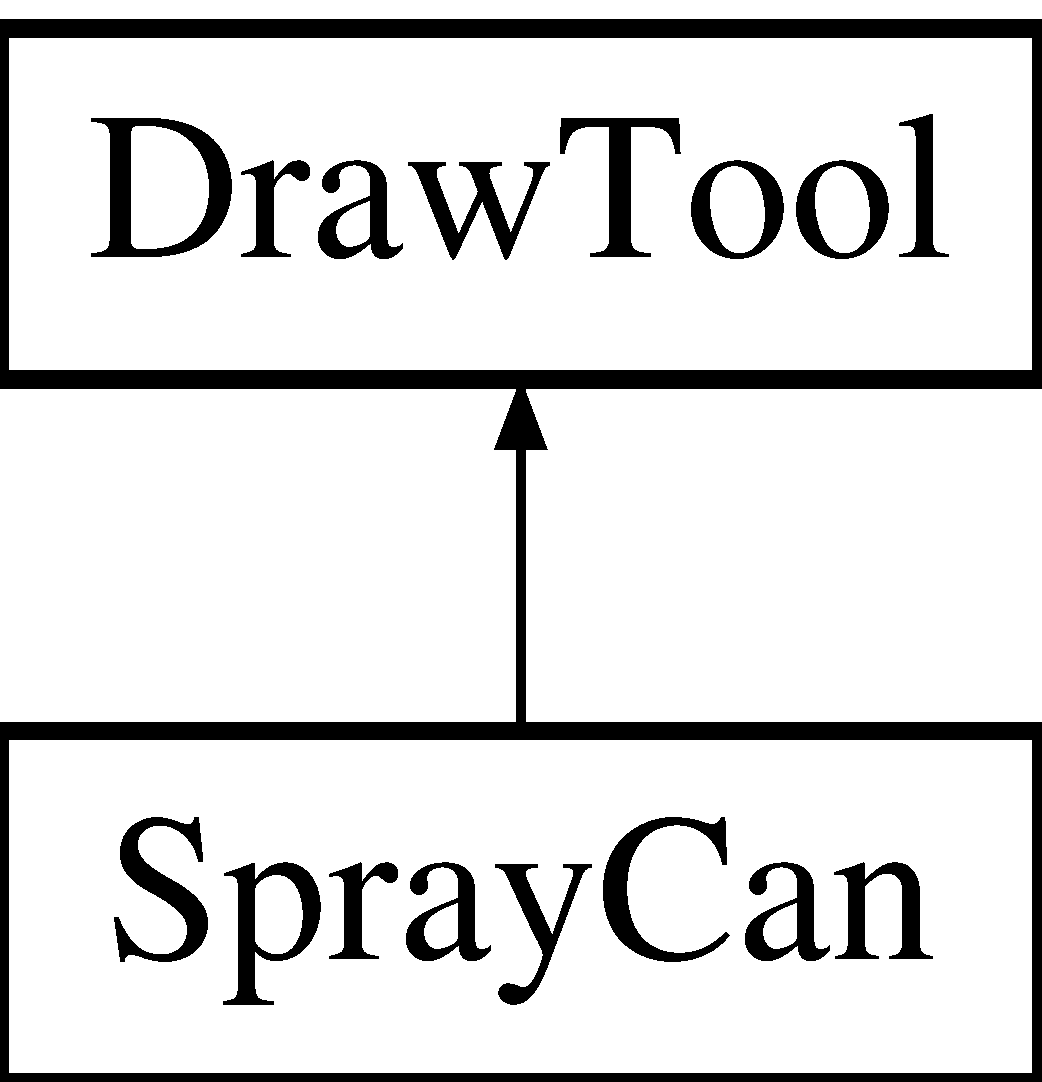
\includegraphics[height=2.000000cm]{classSprayCan}
\end{center}
\end{figure}
\subsection*{Public Member Functions}
\begin{DoxyCompactItemize}
\item 
\hypertarget{classSprayCan_a5491c5e7346fb7126b45405664b22f5d}{{\bfseries Spray\-Can} (\hyperlink{classColorData}{Color\-Data} $\ast$tool\-Color, int radius)}\label{classSprayCan_a5491c5e7346fb7126b45405664b22f5d}

\item 
\hypertarget{classSprayCan_a86321320d34fdc49c754ce6d1ff324fd}{void {\bfseries fill\-Influence} ()}\label{classSprayCan_a86321320d34fdc49c754ce6d1ff324fd}

\item 
\hypertarget{classSprayCan_ade6115cd8e7f277c74b0c6ade3547e2c}{void {\bfseries paint} (int x, int y, int prev\-X, int prev\-Y, \hyperlink{classPixelBuffer}{Pixel\-Buffer} $\ast$buffer)}\label{classSprayCan_ade6115cd8e7f277c74b0c6ade3547e2c}

\item 
\hypertarget{classSprayCan_a6be9bc1725f16fdb0e6f3610fe60e22c}{string {\bfseries get\-Name} ()}\label{classSprayCan_a6be9bc1725f16fdb0e6f3610fe60e22c}

\end{DoxyCompactItemize}
\subsection*{Additional Inherited Members}


The documentation for this class was generated from the following files\-:\begin{DoxyCompactItemize}
\item 
libphoto/Spray\-Can.\-h\item 
libphoto/Spray\-Can.\-cpp\end{DoxyCompactItemize}

\hypertarget{classStamp}{\section{Stamp Class Reference}
\label{classStamp}\index{Stamp@{Stamp}}
}
Inheritance diagram for Stamp\-:\begin{figure}[H]
\begin{center}
\leavevmode
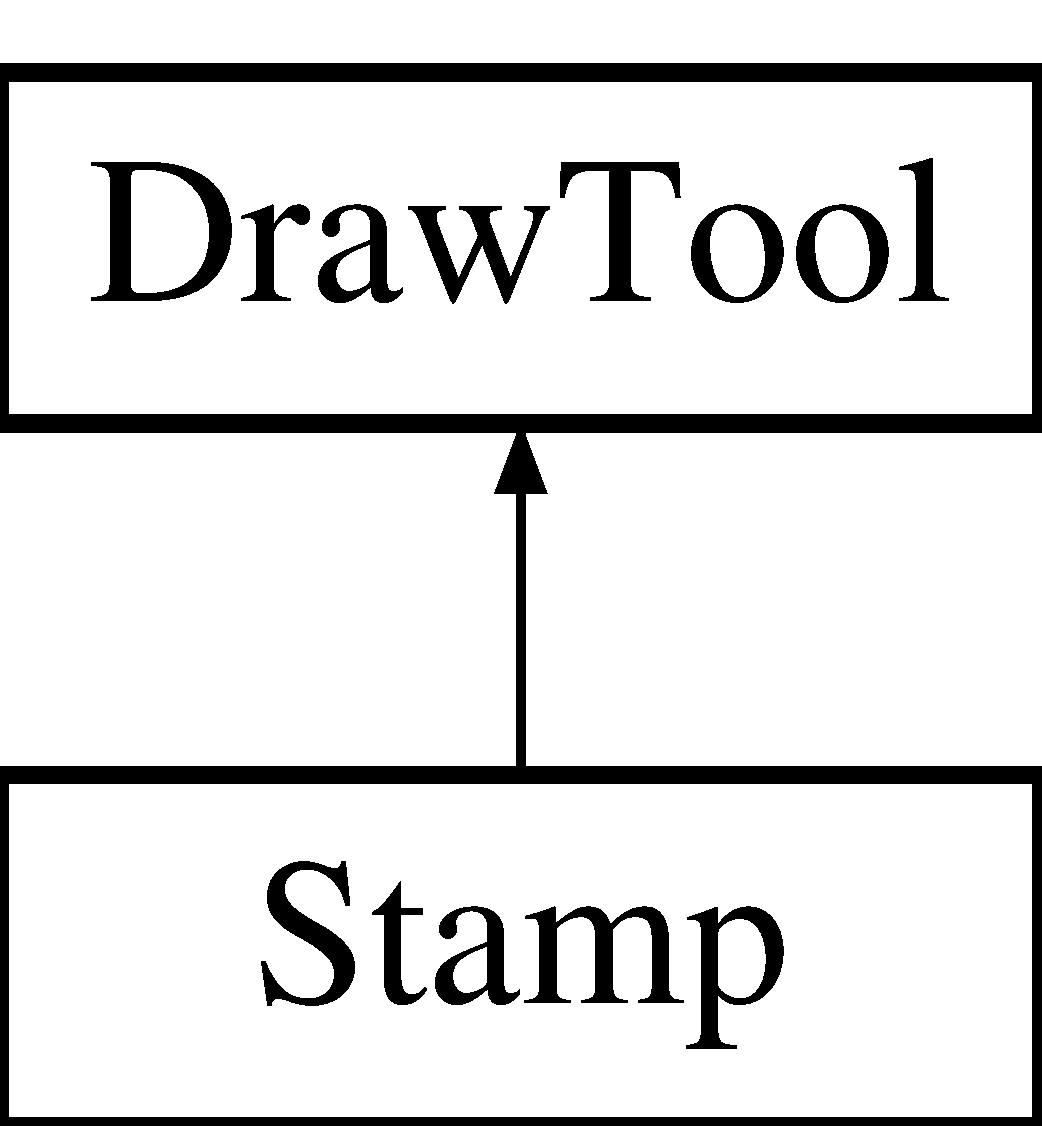
\includegraphics[height=2.000000cm]{classStamp}
\end{center}
\end{figure}
\subsection*{Public Member Functions}
\begin{DoxyCompactItemize}
\item 
\hypertarget{classStamp_a92ac49815361090e983b1adf13451dc5}{{\bfseries Stamp} (\hyperlink{classPixelBuffer}{Pixel\-Buffer} $\ast$new\-Buffer, int stamp\-Width, int stamp\-Height)}\label{classStamp_a92ac49815361090e983b1adf13451dc5}

\item 
\hypertarget{classStamp_a327f68b52c3043a538180461d5b96cb9}{void {\bfseries fill\-Influence} ()}\label{classStamp_a327f68b52c3043a538180461d5b96cb9}

\item 
\hypertarget{classStamp_ab41c9de007e2ad05a6b47e62b41fd7df}{void {\bfseries apply\-Influence} (int x, int y, \hyperlink{classPixelBuffer}{Pixel\-Buffer} $\ast$buffer)}\label{classStamp_ab41c9de007e2ad05a6b47e62b41fd7df}

\item 
\hypertarget{classStamp_a92ac49815361090e983b1adf13451dc5}{{\bfseries Stamp} (\hyperlink{classPixelBuffer}{Pixel\-Buffer} $\ast$new\-Buffer, int stamp\-Width, int stamp\-Height)}\label{classStamp_a92ac49815361090e983b1adf13451dc5}

\item 
\hypertarget{classStamp_a327f68b52c3043a538180461d5b96cb9}{void {\bfseries fill\-Influence} ()}\label{classStamp_a327f68b52c3043a538180461d5b96cb9}

\item 
\hypertarget{classStamp_ab41c9de007e2ad05a6b47e62b41fd7df}{void {\bfseries apply\-Influence} (int x, int y, \hyperlink{classPixelBuffer}{Pixel\-Buffer} $\ast$buffer)}\label{classStamp_ab41c9de007e2ad05a6b47e62b41fd7df}

\item 
\hypertarget{classStamp_a92ac49815361090e983b1adf13451dc5}{{\bfseries Stamp} (\hyperlink{classPixelBuffer}{Pixel\-Buffer} $\ast$new\-Buffer, int stamp\-Width, int stamp\-Height)}\label{classStamp_a92ac49815361090e983b1adf13451dc5}

\item 
\hypertarget{classStamp_a327f68b52c3043a538180461d5b96cb9}{void {\bfseries fill\-Influence} ()}\label{classStamp_a327f68b52c3043a538180461d5b96cb9}

\item 
\hypertarget{classStamp_ab41c9de007e2ad05a6b47e62b41fd7df}{void {\bfseries apply\-Influence} (int x, int y, \hyperlink{classPixelBuffer}{Pixel\-Buffer} $\ast$buffer)}\label{classStamp_ab41c9de007e2ad05a6b47e62b41fd7df}

\end{DoxyCompactItemize}
\subsection*{Additional Inherited Members}


The documentation for this class was generated from the following files\-:\begin{DoxyCompactItemize}
\item 
libphoto/include/libphoto.\-h\item 
libphoto/Stamp.\-h\item 
libphoto/Stamp.\-cpp\end{DoxyCompactItemize}

\hypertarget{classWaterColor}{}\section{Water\+Color Class Reference}
\label{classWaterColor}\index{Water\+Color@{Water\+Color}}
Inheritance diagram for Water\+Color\+:\begin{figure}[H]
\begin{center}
\leavevmode
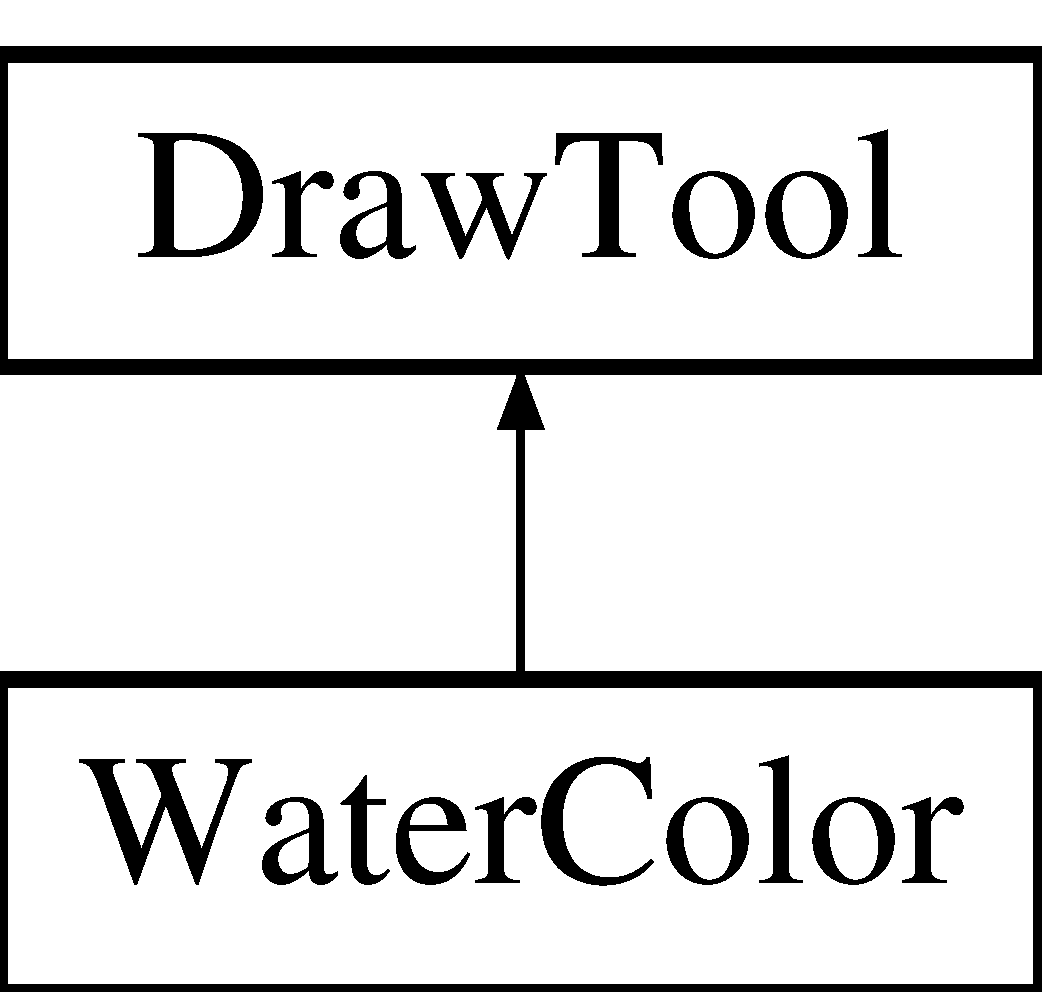
\includegraphics[height=2.000000cm]{classWaterColor}
\end{center}
\end{figure}
\subsection*{Public Member Functions}
\begin{DoxyCompactItemize}
\item 
\hyperlink{classWaterColor_ac61121474a9faeabc3610be7c6dd24b6}{Water\+Color} (\hyperlink{classColorData}{Color\+Data} $\ast$tool\+Color, int radius)
\begin{DoxyCompactList}\small\item\em For function descriptions please see the \hyperlink{classBlur}{Blur} class. \end{DoxyCompactList}\item 
void \hyperlink{classWaterColor_a98f3e467458f9a329c783d1c03af05db}{fill\+Influence} ()
\item 
string {\bfseries get\+Name} ()\hypertarget{classWaterColor_a6827a8d8fc051d1f64314da5d6b0229c}{}\label{classWaterColor_a6827a8d8fc051d1f64314da5d6b0229c}

\end{DoxyCompactItemize}
\subsection*{Additional Inherited Members}


\subsection{Constructor \& Destructor Documentation}
\index{Water\+Color@{Water\+Color}!Water\+Color@{Water\+Color}}
\index{Water\+Color@{Water\+Color}!Water\+Color@{Water\+Color}}
\subsubsection[{\texorpdfstring{Water\+Color(\+Color\+Data $\ast$tool\+Color, int radius)}{WaterColor(ColorData *toolColor, int radius)}}]{\setlength{\rightskip}{0pt plus 5cm}Water\+Color\+::\+Water\+Color (
\begin{DoxyParamCaption}
\item[{{\bf Color\+Data} $\ast$}]{tool\+Color, }
\item[{int}]{radius}
\end{DoxyParamCaption}
)}\hypertarget{classWaterColor_ac61121474a9faeabc3610be7c6dd24b6}{}\label{classWaterColor_ac61121474a9faeabc3610be7c6dd24b6}


For function descriptions please see the \hyperlink{classBlur}{Blur} class. 

This is the watercolor class, it inherits from \hyperlink{classDrawTool}{Draw\+Tool}. It only has to deal with filling its influence, the \hyperlink{classDrawTool}{Draw\+Tool} applies it. 

\subsection{Member Function Documentation}
\index{Water\+Color@{Water\+Color}!fill\+Influence@{fill\+Influence}}
\index{fill\+Influence@{fill\+Influence}!Water\+Color@{Water\+Color}}
\subsubsection[{\texorpdfstring{fill\+Influence()}{fillInfluence()}}]{\setlength{\rightskip}{0pt plus 5cm}void Water\+Color\+::fill\+Influence (
\begin{DoxyParamCaption}
{}
\end{DoxyParamCaption}
)\hspace{0.3cm}{\ttfamily [virtual]}}\hypertarget{classWaterColor_a98f3e467458f9a329c783d1c03af05db}{}\label{classWaterColor_a98f3e467458f9a329c783d1c03af05db}
Virtual function to set influence on the mask, should be overrode in sub class ~\newline
 none ~\newline
 void ~\newline


Reimplemented from \hyperlink{classDrawTool_ae202bc193ba721452e81f34b6c2e6e35}{Draw\+Tool}.



The documentation for this class was generated from the following files\+:\begin{DoxyCompactItemize}
\item 
libphoto/Water\+Color.\+h\item 
libphoto/Water\+Color.\+cpp\end{DoxyCompactItemize}

%--- End generated contents ---

% Index
\newpage
\phantomsection
\addcontentsline{toc}{chapter}{Index}
\printindex

\end{document}
